% Options for packages loaded elsewhere
\PassOptionsToPackage{unicode}{hyperref}
\PassOptionsToPackage{hyphens}{url}
%
\documentclass[
  man,floatsintext]{apa6}
\usepackage{amsmath,amssymb}
\usepackage{iftex}
\ifPDFTeX
  \usepackage[T1]{fontenc}
  \usepackage[utf8]{inputenc}
  \usepackage{textcomp} % provide euro and other symbols
\else % if luatex or xetex
  \usepackage{unicode-math} % this also loads fontspec
  \defaultfontfeatures{Scale=MatchLowercase}
  \defaultfontfeatures[\rmfamily]{Ligatures=TeX,Scale=1}
\fi
\usepackage{lmodern}
\ifPDFTeX\else
  % xetex/luatex font selection
\fi
% Use upquote if available, for straight quotes in verbatim environments
\IfFileExists{upquote.sty}{\usepackage{upquote}}{}
\IfFileExists{microtype.sty}{% use microtype if available
  \usepackage[]{microtype}
  \UseMicrotypeSet[protrusion]{basicmath} % disable protrusion for tt fonts
}{}
\makeatletter
\@ifundefined{KOMAClassName}{% if non-KOMA class
  \IfFileExists{parskip.sty}{%
    \usepackage{parskip}
  }{% else
    \setlength{\parindent}{0pt}
    \setlength{\parskip}{6pt plus 2pt minus 1pt}}
}{% if KOMA class
  \KOMAoptions{parskip=half}}
\makeatother
\usepackage{xcolor}
\usepackage{graphicx}
\makeatletter
\def\maxwidth{\ifdim\Gin@nat@width>\linewidth\linewidth\else\Gin@nat@width\fi}
\def\maxheight{\ifdim\Gin@nat@height>\textheight\textheight\else\Gin@nat@height\fi}
\makeatother
% Scale images if necessary, so that they will not overflow the page
% margins by default, and it is still possible to overwrite the defaults
% using explicit options in \includegraphics[width, height, ...]{}
\setkeys{Gin}{width=\maxwidth,height=\maxheight,keepaspectratio}
% Set default figure placement to htbp
\makeatletter
\def\fps@figure{htbp}
\makeatother
\setlength{\emergencystretch}{3em} % prevent overfull lines
\providecommand{\tightlist}{%
  \setlength{\itemsep}{0pt}\setlength{\parskip}{0pt}}
\setcounter{secnumdepth}{-\maxdimen} % remove section numbering
% Make \paragraph and \subparagraph free-standing
\ifx\paragraph\undefined\else
  \let\oldparagraph\paragraph
  \renewcommand{\paragraph}[1]{\oldparagraph{#1}\mbox{}}
\fi
\ifx\subparagraph\undefined\else
  \let\oldsubparagraph\subparagraph
  \renewcommand{\subparagraph}[1]{\oldsubparagraph{#1}\mbox{}}
\fi
\newlength{\cslhangindent}
\setlength{\cslhangindent}{1.5em}
\newlength{\csllabelwidth}
\setlength{\csllabelwidth}{3em}
\newlength{\cslentryspacingunit} % times entry-spacing
\setlength{\cslentryspacingunit}{\parskip}
\newenvironment{CSLReferences}[2] % #1 hanging-ident, #2 entry spacing
 {% don't indent paragraphs
  \setlength{\parindent}{0pt}
  % turn on hanging indent if param 1 is 1
  \ifodd #1
  \let\oldpar\par
  \def\par{\hangindent=\cslhangindent\oldpar}
  \fi
  % set entry spacing
  \setlength{\parskip}{#2\cslentryspacingunit}
 }%
 {}
\usepackage{calc}
\newcommand{\CSLBlock}[1]{#1\hfill\break}
\newcommand{\CSLLeftMargin}[1]{\parbox[t]{\csllabelwidth}{#1}}
\newcommand{\CSLRightInline}[1]{\parbox[t]{\linewidth - \csllabelwidth}{#1}\break}
\newcommand{\CSLIndent}[1]{\hspace{\cslhangindent}#1}
\ifLuaTeX
\usepackage[bidi=basic]{babel}
\else
\usepackage[bidi=default]{babel}
\fi
\babelprovide[main,import]{english}
% get rid of language-specific shorthands (see #6817):
\let\LanguageShortHands\languageshorthands
\def\languageshorthands#1{}
% Manuscript styling
\usepackage{upgreek}
\captionsetup{font=singlespacing,justification=justified}

% Table formatting
\usepackage{longtable}
\usepackage{lscape}
% \usepackage[counterclockwise]{rotating}   % Landscape page setup for large tables
\usepackage{multirow}		% Table styling
\usepackage{tabularx}		% Control Column width
\usepackage[flushleft]{threeparttable}	% Allows for three part tables with a specified notes section
\usepackage{threeparttablex}            % Lets threeparttable work with longtable

% Create new environments so endfloat can handle them
% \newenvironment{ltable}
%   {\begin{landscape}\centering\begin{threeparttable}}
%   {\end{threeparttable}\end{landscape}}
\newenvironment{lltable}{\begin{landscape}\centering\begin{ThreePartTable}}{\end{ThreePartTable}\end{landscape}}

% Enables adjusting longtable caption width to table width
% Solution found at http://golatex.de/longtable-mit-caption-so-breit-wie-die-tabelle-t15767.html
\makeatletter
\newcommand\LastLTentrywidth{1em}
\newlength\longtablewidth
\setlength{\longtablewidth}{1in}
\newcommand{\getlongtablewidth}{\begingroup \ifcsname LT@\roman{LT@tables}\endcsname \global\longtablewidth=0pt \renewcommand{\LT@entry}[2]{\global\advance\longtablewidth by ##2\relax\gdef\LastLTentrywidth{##2}}\@nameuse{LT@\roman{LT@tables}} \fi \endgroup}

% \setlength{\parindent}{0.5in}
% \setlength{\parskip}{0pt plus 0pt minus 0pt}

% Overwrite redefinition of paragraph and subparagraph by the default LaTeX template
% See https://github.com/crsh/papaja/issues/292
\makeatletter
\renewcommand{\paragraph}{\@startsection{paragraph}{4}{\parindent}%
  {0\baselineskip \@plus 0.2ex \@minus 0.2ex}%
  {-1em}%
  {\normalfont\normalsize\bfseries\itshape\typesectitle}}

\renewcommand{\subparagraph}[1]{\@startsection{subparagraph}{5}{1em}%
  {0\baselineskip \@plus 0.2ex \@minus 0.2ex}%
  {-\z@\relax}%
  {\normalfont\normalsize\itshape\hspace{\parindent}{#1}\textit{\addperi}}{\relax}}
\makeatother

\makeatletter
\usepackage{etoolbox}
\patchcmd{\maketitle}
  {\section{\normalfont\normalsize\abstractname}}
  {\section*{\normalfont\normalsize\abstractname}}
  {}{\typeout{Failed to patch abstract.}}
\patchcmd{\maketitle}
  {\section{\protect\normalfont{\@title}}}
  {\section*{\protect\normalfont{\@title}}}
  {}{\typeout{Failed to patch title.}}
\makeatother

\usepackage{xpatch}
\makeatletter
\xapptocmd\appendix
  {\xapptocmd\section
    {\addcontentsline{toc}{section}{\appendixname\ifoneappendix\else~\theappendix\fi\\: #1}}
    {}{\InnerPatchFailed}%
  }
{}{\PatchFailed}
\usepackage{csquotes}
\usepackage{setspace}
\usepackage{enumitem}
\AtBeginEnvironment{tabular}{\singlespacing}
\AtBeginEnvironment{tabular}{\footnotesize}
\AtBeginEnvironment{lltable}{\singlespacing}
\AtBeginEnvironment{tablenotes}{\singlespacing}
\captionsetup[table]{font={stretch=1}}
\captionsetup[figure]{font={stretch=1}}
\captionsetup[table]{skip=10pt}
\setlist{nolistsep}
\setlist{nosep}
\usepackage{subfig}
\usepackage{float}
\ifLuaTeX
  \usepackage{selnolig}  % disable illegal ligatures
\fi
\IfFileExists{bookmark.sty}{\usepackage{bookmark}}{\usepackage{hyperref}}
\IfFileExists{xurl.sty}{\usepackage{xurl}}{} % add URL line breaks if available
\urlstyle{same}
\hypersetup{
  pdftitle={A Methodological Evaluation of Meta-Analyses in tDCS - Motor Learning Research},
  pdfauthor={Taym Alsalti},
  pdflang={en-EN},
  hidelinks,
  pdfcreator={LaTeX via pandoc}}

\title{A Methodological Evaluation of Meta-Analyses in tDCS - Motor Learning Research}
\author{Taym Alsalti\textsuperscript{}}
\date{}


\shorttitle{M-A Methods in tDCS - Motor Learning Research}

\affiliation{\vspace{0.5cm}\textsuperscript{} Freie Universität Berlin}

\abstract{%
With transcranial direct-current stimulation's (tDCS) rising popularity both in motor learning research and as a commercial product, it is becoming increasingly important that the quality of evidence on its effectiveness be evaluated. Special attention should be paid to meta-analyses, as they usually have a larger impact on research and clinical practice than other types of studies. There is evidence for several methodological issues in the tDCS motor learning literature such as limited reproducibility, largely untested replicability, and marked hetereogeneity in the technical paramaters employed. These issues inevitably impact the quality of the meta-analyses synthesising these studies, which display methodological problems of their own. The aim of this project was to evaluate the methodological quality of meta-analyses estimating the effect of tDCS on motor learning with respect to three main aspects: reporting quality, reproducibility, and publication bias control. Akin to previous reviews with similar aims, we show that the methods and results sections of meta-analyses are severely underreported, which compromises the ability to judge the soundness of the methodogloical procedure adopted as well as its reproducibility. Furthermore, only one of the three meta-analyses reported having taken non-statistical approaches to control for publication bias and all three used older statistical methods which are known to produce results of limited validity. These results reemphasise the need to evaluate the quality of meta-analyses as they have the largest impact on research, clinical practice, and even consumer behaviour.
}



\begin{document}
\maketitle

\hypertarget{introduction}{%
\section{Introduction}\label{introduction}}

\hypertarget{transcranial-direct-current-stimulation}{%
\subsection{Transcranial direct-current stimulation}\label{transcranial-direct-current-stimulation}}

Transcranial direct-current stimulation (tDCS) refers to a non-invasive brain stimulation technique which involves delivering constant, low current to the brain via electrodes fixed on the scalp (Gazzaniga, Ivry, \& Mangun, 2018). tDCS is believed to be capable of both temporarily and permanently altering brain function by increasing or decreasing excitability in targeted cortical regions depending on the type of stimulation implemented (Stagg \& Nitsche, 2011). Positive current delivered via the anodal electrode causes neurons just beneath the region stimulated to depolarise, that is, to increase their excitability, rendering them more likely to start off an action potential. Neurons targeted by negative stimulation, on the other hand, become hyperpolerised, i.e., less likely to ``fire'' (Gazzaniga et al., 2018). An important third type of stimulation is sham stimulation, which involves delivering an initial brief current that quickly fades off, leaving an inactive electrode for the remainder of the experiment. Sham stimulation is used as the control condition in experimental settings. tDCS is known to be safe and to cause negligible side-effects, if any (Gianni et al., 2021; Nitsche et al., 2008).

The typical set-up of a tDCS protocol involves no more than a handful of inexpensive components and relatively simple steps (Gebodh et al., 2019; Woods et al., 2016). A standard tDCS device consists of an anodal (positively charged) and a cathodal (negatively charged) electrode attached to a battery-powered device which controls the type and intensity of the current as well as the duration of the stimulation. To ensure that the administered current actually reaches the target area, a few measures are usually taken to minimise resistance between the skin and the active electrodes. This includes using a sponge and an electrolyte-based contact medium such as gel and any materials necessary to make sure the electrodes remain fixed in their positions. Electroencephalography (EEG) or magnetic resonance imaging (MRI) is sometimes used to more accurately locate the region of interest or to monitor the physiological effects of tDCS in real time (Nitsche et al., 2008; Woods et al., 2016). More recent variations of tDCS used for at-home clinical interventions are even simpler (Riggs et al., 2018).
\vspace{-1mm}

When considering these advantages, tDCS's rapidly increasing popularity over the last two decades is not surprising (Buch et al., 2017). In clinical research, its efficacy for treating or attenuating depression (Brunoni et al., 2016), memory deficits in Alzheimer's patients (Bennabi et al., 2014), pain (Luedtke et al., 2012), schizophrenia (Liu et al., 2021), and others, has been investigated. Interest in tDCS was not restricted to clinical settings: studies on healthy subjects have been conducted to test its effects on cognitive abilities such as language and memory (Horvath, Forte, \& Carter, 2015), affective states (Austin et al., 2016), and motor skills, such as surgery (Hung et al., 2021a) and musical performance (Rosen et al., 2016).

Indeed, tDCS has become so established as a research tool that it is already approved for clinical use (with some restrictions) in several countries around the world (Fregni et al., 2015). Furthermore, an ever-richer variety of commercial tDCS products has become available on the market (Davis, 2016; Wexler, 2018; Zettler, 2017), prompting experts (Wurzman, Hamilton, Pascual-Leone, \& Fox, 2016) to voice concerns over the increasing prevalence of this ``do-it-yourself'' use of tDCS. Out of the 449 such at-home tDCS consumers surveyed by Wexler (2018), 52\% (237) did so for enhancement purposes. It appears likely that this ``hype'' surrounding tDCS products is partly due to considerable media coverage (Dubljević, Saigle, \& Racine, 2014; Steenbergen et al., 2016).

\hypertarget{tdcs-and-motor-learning}{%
\subsection{tDCS and motor learning}\label{tdcs-and-motor-learning}}

One increasingly prevalent implementation of tDCS is to improve motor learning, that is, the acquisition of new motor skills or the improvement of existing ones. Here, complexity is compounded by the multifacetedness of motor skills and the variety of ways to measure them (Buch et al., 2017). They can range from the most mundane daily activities like walking or doing the dishes to finer skills that can require years to master such as playing a musical instrument or performing surgery. tDCS is most often used as a supplement to specialised training (Buch et al., 2017). The two main types of improvement that can occur are referred to as ``online learning'' (improvement over short time periods such as within a single training session or a day) and consolidated learning (over several hours, days, or training sessions).

Experimental paradigms aiming to evaluate such patterns of improvement typically take the following form (Buch et al., 2017; Reis et al., 2009): following baseline measurements of different outcomes on the first day, study participants undergo a series of training sessions in a specific motor task (e.g., squeezing a hand-held force transducer to move the cursor on the computer screen quickly and accurately between a starting position and a target position). The participants receive tDCS (or sham, depending on group and time point) during this training. Performance is measured subsequently (online) and/or 1 to several weeks or months later (consolidation/retention).
Measuring motor learning is a complex task, too, as motor skills require an optimisation of a speed-accuracy trade-off. Different tasks and measurement instruments take this into account in different ways depending on context. For example, some tasks involve instructing participants to focus on either speed or accuracy. Another approach is to stick to neutral instructions and instead explicitly model this trade-off, as done by Reis et al. (2009):
\[ 
\textrm{skill} = \frac{1-\textrm{error rate}}{\textrm{error rate}(\ln(\textrm{duration})^b)}
\tag{1}
\]
Where \(b\) is a fixed constant.

\newpage

\hypertarget{issues-in-tdcs-research}{%
\subsection{Issues in tDCS research}\label{issues-in-tdcs-research}}

Although tDCS might hold promise for those and other applications, treating tDCS's positive effects as an established fact is deemed by experts in the field as premature (Buch et al., 2017). The technique's apparent simplicity might lead researchers to disregard aspects which are crucial to obtaining reliable results (Gebodh et al., 2019; Woods et al., 2016). When conducting a tDCS experiment, the researcher must select the type of stimulation, electrode size, shape and material; the duration of the stimulation; the location of the electrodes; and the current intensity, all of which are factors that have a substantial impact on stimulation efficacy.

The wide range of different possible tDCS settings appears to be well utilised by researchers as there is evidence of considerable heterogeneity in the literature with respect to tDCS-related parameters, tasks, and outcomes (Buch et al., 2017). tDCS research also appears to suffer from the same methodological problems as neighbouring fields in the behavioural and cognitive (neuro)sciences, such as suboptimal reproducibility, untested replicability, underpowered studies (Minarik et al., 2016), and publication bias (Button et al., 2013). These issues make it difficult to evaluate the evidence or reach conclusions based on it. They also hamper cumulative science as it is difficult to synthesise the results of studies for the purpose of a meta-analysis when they vary too much in quality and methodological approach (Borenstein, Hedges, Higgins, \& Rothstein, 2009b).

\hypertarget{meta-analysis}{%
\subsection{Meta-analysis}\label{meta-analysis}}

Meta-analysis refers to a method of quantitatively synthesising the results of a set of studies while weighing individual studies differently depending on certain criteria (Borenstein \& Hedges, 2019). The most common measure used for weighing effect sizes derived from primary studies is the sampling variance, which is largely dependent on the study's sample size. For example, should one wish to estimate the effect on an intervention based on multiple studies with a control group, a common procedure would be to calculate a standardised mean difference (SMD) in the form of a Cohen's \(d\):
\[
d={\frac {{\bar{x}}_{t}-{\bar{x}}_{c}}{s}} 
\tag{2}
\]
\[
s={\sqrt {\frac {(n_{t}-1)s_{t}^{2}+(n_{c}-1)s_{c}^{2}}{n_{t}+n_{c}-2}}}
\tag{3}
\]
Where \({\bar{x}}_{t}\) is the mean of the treatment group, \({\bar{x}}_{c}\) is the mean of the control group, \(s\) is the pooled standard deviation, \(n_{t}\) and \(n_{c}\) are the sample sizes of the treatment and control groups, respectively, and \(s_{t}\) and \(s_{c}\) are the standard deviations of the treatment and control groups, respectively.

The next step would be to calculate the inverse-variance weight \(w=\frac{1}{v_i}\) for each \(d\), where the sampling variance \(v_i\) is conventionally calculated via:
\[
v_i={\frac{n_{t}+n_{c}}{n_{t}n_{c}}}v
\tag{4}
\]
Where \(v\) represents the pooled variance of the two groups. One can then calculate the pooled Cohen's \(d\) using the primary \(d\)s and their corresponding weights:
\[
\bar{d}={\frac{\sum_{i=1}^{k}w_id_i}{\sum_{i=1}^{k}w_i}}
\tag{5}
\]
This would be a so-called fixed-effects meta-analytic model, under which one assumes the primary effect sizes to stem from a single common true effect size (Konstantopoulos \& Hedges, 2019). On the other hand, the true effect effect size is itself random and has its own distribution under a random-effects model. Computationally, the only difference between a fixed-effects and a random-effects model is that for the purpose of the latter, the sampling variances \(v^*_i\) are formed by adding to the fixed-effects sampling variance a between-study variance component \(\tau^2\). There are about a dozen different methods to estimate the between-study heterogeneity, see Veroniki et al. (2016) for an overview.

Meta-analysis studies merit special scrutiny and should be invariably executed to the highest standards as they are usually cited more frequently than primary studies about the same topics, are commonly assumed to provide the most accurate estimate of an effect, and have a large impact on theory development as well as policy and clinical practice (Gopalakrishnan \& Ganeshkumar, 2013; Gøtzsche, Hróbjartsson, Marić, \& Tendal, 2007; Ioannidis, 2016; Lakens et al., 2017; Morganti, 2007). However, meta-analyses can and often \emph{do} suffer from methodological problems which go beyond those of the primary studies they synthesise (Ioannidis, 2016). Here, we focused on the issues of reporting quality, reproducibility, and publication bias control.
\vspace{-5mm}

\hypertarget{reporting-quality}{%
\subsection{Reporting quality}\label{reporting-quality}}

One crucial issue is reporting completeness describing the used methods and the results. Researchers must make a great number of decisions at multiple stages of a study's timeline. These decisions impact the outcome of the study to various degrees and only by providing a full, justified account of which path was taken at each fork can other researchers evaluate the soundness of the methodological approach (Botvinik-Nezer et al., 2020; Gelman \& Loken, 2013; Hyatt et al., 2020; Simmons, Nelson, \& Simonsohn, 2011). Meta-analysts in particular are faced with a plethora of different decisions with regards to which databases to search and using which strings; primary study selection and exclusion; data extraction; statistical methods, among others (Ada, Sharman, \& Balkundi, 2012; Geyskens, Krishnan, Steenkamp, \& Cunha, 2009; Guzzo, Jackson, \& Katzell, 1987; Nieminen, Nicklin, McClure, \& Chakrabarti, 2011; Schalken \& Rietbergen, 2017; Valentine, Pigott, \& Rothstein, 2010; Voracek, Kossmeier, \& Tran, 2019). Although the extent to which these ``researcher degrees of freedom'' (Simmons et al., 2011) impact the conclusions of the meta-analysis is not a completely uncontroversial issue\footnote{One review of meta-analyses in the organisational sciences found that 21 different analytical decisions have a negligible impact on the pooled ES estimate (Aguinis, Dalton, Bosco, Pierce, \& Dalton, 2011)}, there is consensus regarding the importance of transparently reporting these decisions (Aguinis, Pierce, Bosco, Dalton, \& Dalton, 2011), as it is difficult to assess the quality and trustworthiness of that which one does not have access to (Page, McKenzie, et al., 2021).

Hundreds of different sets of reporting guidelines have been developed for different types of studies conducted across various fields (\emph{Reporting Guidelines \textbar{} {The EQUATOR Network}}, n.d.) including several for meta-analyses, for example, the Cochrane Handbook (Higgins et al., 2019), Preferred Reporting Items for Systematic Reviews and Meta-Analyses (PRISMA, Moher et al., 2000; Moher, Liberati, Tetzlaff, Altman, \& Group, 2009; Page, McKenzie, et al., 2021), Meta-Analysis Reporting Standards (MARS, American Psychological Association, n.d.), with PRISMA being the most widely known and adopted (Page \& Moher, 2017).

PRISMA's predecessor, The Quality of Reports of Meta-analyses Statement (QUOROM, Moher et al., 2000), was developed in response to a rapidly rising number of meta-analyses with widely varying degrees of reporting completeness. The statement proceeded from a conference held to discuss these issues surrounding research synthesis, especially randomised controlled trials (RCTS). Its aim was to provide meta-analysts with help to better report their studies.
This help came in the form of a flow diagram of the different stages of a meta-analysis and a checklist. The checklist includes 18 items about how the different sections of the meta-analytic study should look like.

The updated versions of the reporting guidelines (rebranded as PRISMA to encompass reviews without quantitative synthesis, Moher et al., 2009; Page, McKenzie, et al., 2021) elaborated on both the checklist and the flow chart (see Figure 1 for the 2009 edition). Here we focused on the 2009 version of PRISMA as we expected most meta-analyses we evaluated to be published after 2009 but before 2020.
\newpage

\begin{figure}[H]

{\centering 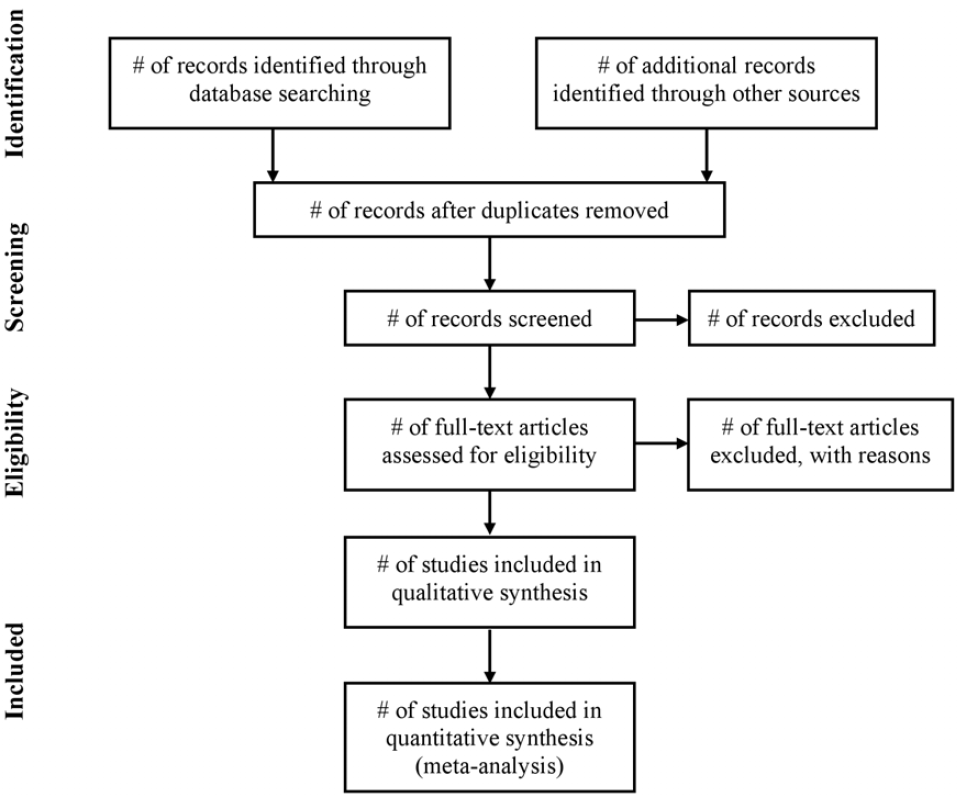
\includegraphics[width=0.85\linewidth]{figures/prisma} 

}

\caption{PRISMA flow chart of the meta-analytical process. Adapted as is from Moher et al. (2009).}\label{fig:fig1}
\end{figure}

The 2009 PRISMA (henceforth simply PRISMA) checklist included 27 items (see Table 1), with 12 of them pertaining to methods and 7 to results. We paid special attention to items 6 to 9 and 17 as they pertain to important methodological aspects (study selection) and are not covered by our evaluation of reproducibility.

\newpage
\singlespacing
\begingroup\fontsize{10}{12}\selectfont

\begin{longtable}[t]{>{\raggedleft\arraybackslash}p{5em}>{\raggedright\arraybackslash}p{5em}>{\raggedright\arraybackslash}p{32em}}
\caption{\label{tab:table1}PRISMA (Moher et al., 2009) checklist.}\\
\toprule
Item number & Section & Original description of item\\
\midrule
\endfirsthead
\caption[]{\label{tab:table1}PRISMA (Moher et al., 2009) checklist. \textit{(continued)}}\\
\toprule
Item number & Section & Original description of item\\
\midrule
\endhead
\midrule
\multicolumn{3}{r@{}}{}\
\endfoot
\bottomrule
\endlastfoot
1 & Title & Identify the report as a systematic review, meta-analysis, or both.\\
2 & Abstract & Provide a structured summary including, as applicable: background; objectives; data sources; study eligibility criteria, participants, and interventions; study appraisal and synthesis methods; results; limitations; conclusions and implications of key findings; systematic review registration number.\\
3 & Introduction & Describe the rationale for the review in the context of what is already known.\\
4 & Introduction & Provide an explicit statement of questions being addressed with reference to participants, interventions, comparisons, outcomes, and study design (PICOS).\\
5 & Methods & Indicate if a review protocol exists, if and where it can be accessed (e.g., Web address), and, if available, provide registration information including registration number.\\
6 & Methods & Specify study characteristics (e.g., PICOS, length of follow-up) and report characteristics (e.g., years considered, language, publication status) used as criteria for eligibility, giving rationale.\\
7 & Methods & Describe all information sources (e.g., databases with dates of coverage, contact with study authors to identify additional studies) in the search and date last searched.\\
8 & Methods & Present full electronic search strategy for at least one database, including any limits used, such that it could be repeated.\\
9 & Methods & State the process for selecting studies (i.e., screening, eligibility, included in systematic review, and, if applicable, included in the meta-analysis).\\
10 & Methods & Describe method of data extraction from reports (e.g., piloted forms, independently, in duplicate) and any processes for obtaining and confirming data from investigators.\\
11 & Methods & List and define all variables for which data were sought (e.g., PICOS, funding sources) and any assumptions and simplifications made.\\
12 & Methods & Describe methods used for assessing risk of bias of individual studies (including specification of whether this was done at the study or outcome level), and how this information is to be used in any data synthesis.\\
13 & Methods & State the principal summary measures (e.g., risk ratio, difference in means).\\
14 & Methods & Describe the methods of handling data and combining results of studies, if done, including measures of consistency (e.g., 12) for each meta-analysis.\\
15 & Methods & Specify any assessment of risk of bias that may affect the cumulative evidence (e.g., publication bias, selective reporting within studies).\\
16 & Methods & Describe methods of additional analyses (e.g., sensitivity or subgroup analyses, meta-regression), if done, indicating which were pre-specified.\\
17 & Results & Give numbers of studies screened, assessed for eligibility, and included in the review, with reasons for exclusions at each stage, ideally with a flow diagram.\\
18 & Results & For each study, present characteristics for which data were extracted (e.g., study size, PICOS, follow-up period) and provide the citations.\\
19 & Results & Present data on risk of bias of each study and, if available, any outcome level assessment (see item 12).\\
20 & Results & For all outcomes considered (benefits or harms), present, for each study: (a) simple summary data for each intervention group (b) effect estimates and confidence intervals, ideally with a forest plot.\\
21 & Results & Present results of each meta-analysis done, including confidence intervals and measures of consistency.\\
22 & Results & Present results of any assessment of risk of bias across studies (see Item 15).\\
23 & Results & Give results of additional analyses, if done (e.g., sensitivity or subgroup analyses, meta-regression [see Item 16]).\\
24 & Discussion & Summarize the main findings including the strength of evidence for each main outcome; consider their relevance to key groups (e.g., healthcare providers, users, and policy makers).\\
25 & Discussion & Discuss limitations at study and outcome level (e.g., risk of bias), and at review-level (e.g., incomplete retrieval of identified research, reporting bias).\\
26 & Discussion & Provide a general interpretation of the results in the context of other evidence, and implications for future research.\\
27 & Funding & Describe sources of funding for the systematic review and other support (e.g., supply of data); role of funders for the systematic review.\\*
\end{longtable}

Describe sources of funding for the systematic review and other support (e.g., supply of data); role of funders for the systematic review.\textbackslash*
\textbackslash end\{longtable\}
\endgroup{}
\doublespacing

Although QUOROM and other reporting guidelines have been available for over two decades, meta-scientific evaluations of adherence to PRISMA and other guidelines have shown that reporting standards of meta-analyses are generally suboptimal and that these guidelines are rarely fully adhered to (see Table 2 for an overview of such studies). For example, the most extensive review of adherence to PRISMA (Page \& Moher, 2017), which aggregated the results of 57 meta-scientific reviews (which included a total of 6487 systematic reviews) with this research question, found that 11 items were adhered to by less than 67\% of the systematic reviews. These include item 5 (methods: protocol and pre-registration, \textless10\% of systematic reviews), item 8 (methods: search, \textless50\%), item 11 (methods: data items, \textless65\%), item 12 (methods: risk of bias in individual studies, \textless67\%), item 15 (methods: risk of bias across studies, \textless50\%), item 16 (methods: additional analyses, \textless50\%), among others. Items 6 (methods: eligibility criteria), 7 (methods: information sources), 9 (methods: study selection), and 17 (results: study selection) were adhered to in \textasciitilde85\%, \textasciitilde85\%, \textasciitilde67\%, and \textasciitilde72\% of the systematic reviews.

\renewcommand{\arraystretch}{2}
\singlespacing

\begin{longtable}[t]{>{\raggedright\arraybackslash}p{11em}>{\raggedright\arraybackslash}p{13em}>{\raggedright\arraybackslash}p{13em}}
\caption{\label{tab:table2}Studies on reporting quality and adherence to reporting standards.}\\
\toprule
Review & Methods & Conclusions\\
\midrule
Organisational sciences: Aytug et al. (2012); Kepes et al. (2013); Schalken \& Rietbergen (2017) & Reviewed the reporting quality and adherence to MARS guidelines of meta-analyses. & Inadequate reporting and adherence to guidelines.\\
Educational science: Ahn et al. (2012) & Reviewed the methodological quality of meta-analyses. & "[the meta-analyses] followed general recommendations fairly well in problem formulation and data collection, but much improvement is needed in data evaluation and analysis."\\
Psychological science: Dieckmann et al. (2009); Hohn et al. (2020); Polanin et al. (2020) & Reviewed the quality of reporting and methods used in meta-analyses, respectively. & Considerable variability in transparency and methods used. Still insufficient despite improvements over the years.\\
Biomedical sciences: Page \& Moher (2017); Pussegoda et al. (2017) & Summarised the findings of meta-research reviews on the adherence of systematic reviews and meta-analyses to reporting guidelines. & Reporting of several PRISMA items is suboptimal. Reporting quality varied substantially across items of 4 well known sets of reporting guidelines.\\
\bottomrule
\end{longtable}
\doublespacing

\hypertarget{reproducibility}{%
\subsection{Reproducibility}\label{reproducibility}}

A related issue is that the less information a meta-analyst provides about their analytical procedures, the harder it is to reproduce their meta-analysis (Aguinis, Pierce, et al., 2011; Gøtzsche et al., 2007; Lakens et al., 2017; Maassen, Assen, Nuijten, Olsson-Collentine, \& Wicherts, 2020). Reproducibility (and relatedly, replicability) remain a hot topic in the behavioural and biomedical sciences, with various fuzzy or inconsistent definitions still floating around (Goodman, Fanelli, \& Ioannidis, 2016; Plesser, 2018). Both terms have been somewhat indiscriminately used to refer to the ability to obtain the same results of a given study by repeating its described procedure. One widely adopted way to distinguish them is by defining reproducibility as the ability to obtain the numerical findings of the original work using their methods (and if applicable, data pre-processing and analysis code) and the original data. (Direct) replication, on the other hand, refers to repeating the entire study using \emph{new data}. (Broman et al., 2017).

This definition, however, does not do full justice to the nuances of the concept of reproducibility. Importantly, it fails to account for the different types of reproducibility and emphasises one type in particular: \emph{results reproducibility} (Goodman et al., 2016). Two further types can be differentiated: \emph{methods reproducibility}, which refers to ``the provision of enough detail about study procedures and data so the same procedures could, in theory or in actuality, be exactly repeated'' (Goodman et al., 2016, p. 2), and \emph{inferential reproducibility}, which describes the ability to draw ``qualitatively similar conclusions from either an independent replication of a study or a reanalysis of the original study'' (Goodman et al., 2016, p. 4). For example, a study might report its methods extensively enough for it to be easily reproducible methodologically, but for which one obtains different results from the original upon a reproduction attempt. This could occur due to erroneous descriptions of methods or mistakes in the implementation of the described methods.

Similarly, inferential reproducibility can depend on the magnitude of the effect reported in a given study as two interpreters of the same results might be in stark disagreement regarding the inferences which can be drawn from them. A \(p\)-value of 0.04, for example, might have an entirely different ``significance'' for a hard frequentist than for a more Bayes-inclined researcher. Another limitation to the definition above is its implication of a dichotomous nature of reproducibility. Especially with regards to methods and inferential reproducibility, it is somewhat imprudent to think of reproducibility as a binary feature since there are many factors (see methodological decisions discussed above) that might play a role in deeming a study reproducible or not (Broman et al., 2017). Concretely, although it is possible to construct a framework which allows one to make an unambiguous yes or no decision when the results of a study are reproducible (e.g., see Steiner, Wong, \& Anglin, 2019), methods reproducibility is better served by considering it as a function of how much information is provided about the methodological procedure.

Applied to meta-analysis, evaluating all types of reproducibility involves attempting to repeat 1. study search, 2. study screening and selection, 3. data extraction, 4. computing ES estimates for each primary study included (primary ES), 5. computing the main pooled ES estimate (pooled ES), and often 6. computing ``corrected'' pooled ESs, 7. computing multiple pooled ESs based on study characteristics and/or conducting subgroup analyses (Cooper, Hedges, \& Valentine, 2009). Here, the issue of reproducibility acquires yet another layer of complexity: reproducibility with regards to elements 3 to 7 depends not only on what is reported in the meta-analysis, but also what is reported in the included primary studies. How hard it is to reproduce a primary ES, for example, is a function of the amount and precision of the information the meta-analysts reported about how they computed the ES \emph{and} the degree to which this information corresponds to data that is accessible in the primary study.

Several reviews testing the reproducibility of meta-analyses have been conducted (Gøtzsche et al., 2007; Lakens et al., 2017; Maassen et al., 2020, see Table 3)\footnote{Three further relevant reviews in the biomedical sciences were identified after the study was done and could not have influenced our approach: two evaluating the methodological reproducibility of meta-analyses (Page et al., 2018; i.e., without attempting to actually reproduce them, Wayant, Page, \& Vassar, 2019) and one testing the reproducibility of entire meta-analyses (i.e., including study search and screening, Ford, Guyatt, Talley, \& Moayyedi, 2010). These reviews, too, reached the conclusion that meta-analysis reproducibility is mostly limited.}. They emphasised somewhat different methodological aspects (e.g., complete reporting vs.~computational correctness) but were uniform in their focus on reproducing data extraction and ES computation (both primary and pooled). Their conclusions about the reproducibility of meta-analyses were, although of varyingly grave consequences, also similar: the reproducibility of meta-analyses was severely limited due to under-reporting of methods and results as well as errors.
Despite the growing popularity of tDCS and the ensuing increase in number of meta-analyses estimating its effect on motor learning, no evaluation of the reporting quality or reproducibility of meta-analyses in this field has been conducted as far as we are aware.

\singlespacing
\begingroup\fontsize{10}{12}\selectfont

\begin{longtable}[t]{>{\raggedright\arraybackslash}p{5em}>{\raggedright\arraybackslash}p{12.5em}>{\raggedright\arraybackslash}p{12.5em}>{\raggedright\arraybackslash}p{12.5em}}
\caption{\label{tab:table3}Studies on reproducibility of meta-analyses.}\\
\toprule
Review & Methods & Findings & Reasons for Reproducibility\\
\midrule
\endfirsthead
\caption[]{\label{tab:table3}Studies on reproducibility of meta-analyses. \textit{(continued)}}\\
\toprule
Review & Methods & Findings & Reasons for Reproducibility\\
\midrule
\endhead
\midrule
\multicolumn{4}{r@{}}{}\
\endfoot
\bottomrule
\endlastfoot
Gøtzsche et al. (2007) & Attempted to reproduce some of the SMDs reported in 27 biomedical meta-analyses with the objective of testing whether whether SMDs in meta-analyses are accurate. Contacted authors of meta-analyses to acquire unreported information. & "In total, 17 meta-analyses (63\%) had errors for at least 1 of the 2 trials examined. For the 10 meta-analyses with errors of at least 0.1, we checked the data from all the trials and conducted our own meta-analysis, using the authors’ methods. Seven of these 10 meta-analyses were erroneous (70\%); 1 was subsequently retracted, and in 2 a significant difference disappeared or appeared." & "Common problems were erroneous number of patients, means, SDs [standard deviations], and sign for the effect estimate."\\
Lakens et al. (2017) & Attempted to reproduce all primary ESs as well as the pooled ES reported in 20 psychological meta-analyses. More emphasis on transparent reporting of methods and results than on correctness of analysis: classified meta-analyses that did not report primary ESs for each included study as not reproducible. & - "Five of the 20 randomly selected meta-analyses we attempted to reproduce could not be reproduced at all […]"

- "[…] differences between the reported and reproduced ES or sample size were common" & “[meta-analyses could not be reproduced] due to lack of access to raw data, no details about the ESs extracted from each study, or a lack of information about how ESs were coded\\
Maassen et al. (2020) & Attempted to reproduce 500 primary ESs reported in 33 psychological meta-analyses. Only included meta-analyses that reported primary ESs for each included primary study. Distinguished between irreproducibility of a primary ES due to lack of information and irreproducibility due to incorrect calculations. & 234 out of the 500 primary ESs could not be reproduced. & 54 out of the 234 could not be reproduced due to lack of necessary information (e.g., standard deviations in primary study not reported), 74 were incorrect (reproduced ES different to reported), 96 were “ambiguous”, that is, “it was unclear what procedure was followed by the meta-analysts.”\\*
\end{longtable}

\begin{enumerate}
\def\labelenumi{(\arabic{enumi})}
\setcounter{enumi}{2019}
\tightlist
\item
  \& Attempted to reproduce 500 primary ESs reported in 33 psychological meta-analyses. Only included meta-analyses that reported primary ESs for each included primary study. Distinguished between irreproducibility of a primary ES due to lack of information and irreproducibility due to incorrect calculations. \& 234 out of the 500 primary ESs could not be reproduced. \& 54 out of the 234 could not be reproduced due to lack of necessary information (e.g., standard deviations in primary study not reported), 74 were incorrect (reproduced ES different to reported), 96 were ``ambiguous'', that is, ``it was unclear what procedure was followed by the meta-analysts.''\textbackslash*
  \textbackslash end\{longtable\}
  \endgroup{}
  \doublespacing
\end{enumerate}

\hypertarget{publication-bias-control}{%
\subsection{Publication bias control}\label{publication-bias-control}}

Beyond transparency in reporting and any effect it may have on reproducibility, a further issue that merits consideration when evaluating the methodology of meta-analyses is how the meta-analysts dealt with publication bias. Publication bias, that is, the tendency of researchers to suppress findings that do not go their way (``negative'' results) and journals to selectively publish studies that report significant results, has been known to distort the scientific literature for over six decades, having been first discussed in 1959 by Sterling. It remains a major concern, especially in the ``softer'' social sciences (Fanelli, 2010), where the proportion of studies reporting ``positive'' results is markedly higher than in the physical sciences. This remarkably elevated rate of positive results combined with the meagre average power of studies in the behavioural and neurosciences give a clear indication of the presence of publication bias (Button et al., 2013; Szucs \& Ioannidis, 2017; Szucs \& Ioannidis, 2020).

Since this apparent overrepresentation of positive results can (and often does) inflate the ES estimates of meta-analyses in a certain direction (Borenstein, Hedges, Higgins, \& Rothstein, 2009a; Friese \& Frankenbach, 2020; Vevea, Coburn, \& Sutton, 2019), meta-analysis reporting guidelines such as PRISMA have consistently recommended reporting any attempts to account for publication bias (Moher et al., 2000, 2015; Page, McKenzie, et al., 2021). Meta-analysts have at their disposal several measures they can take to mitigate the ubiquitous effects of publication bias. Locating as many unpublished studies as possible is likely to be the most effective method and searching repositories of potentially unpublished results are mandatory (e.g., ClinicalTrials.gov) when conducting a Cochrane systematic review (Higgins et al., 2019). Other such non-statistical approaches to minimising the effect of publication bias include searching pre-print and theses repositories, contacting authors of relevant studies to inquire about potentially file-drawered studies, not restricting the study search to articles written in English, etc..

This endeavour proving fruitless, the meta-analyst may next (or in addition) attempt to detect the presence of publication bias and/or adjust the meta-analytic ES estimate for it statistically. Many procedures for this purpose have been developed in the last three decades displaying varying performance in general and under certain conditions (for extensive reviews/comparisons of these methods see Carter, Schönbrodt, Gervais, \& Hilgard, 2019; Harrer, Cuijpers, Furukawa, \& Ebert, 2021; Marks-Anglin \& Chen, 2020; McShane, Böckenholt, \& Hansen, 2016; Renkewitz \& Keiner, 2019; Vevea et al., 2019). In the following, we will briefly introduce the methods used either in the meta-analyses we reviewed or by us.

These statistical methods can be divided into two main categories: small-study effects-based and \(p\)-values-based. Small-study effect methods have been available for more than two decades and are very widely used {[}at least among the \textasciitilde50\% of meta-analyses which conduct such analyses pageEvaluationsUptakeImpact2017; Vevea et al. (2019); Borenstein et al. (2009a); Harrer et al. (2021){]}. In essence, they are based on the often observed positive correlation between the ES derived from a primary study and the ES's standard error (SE, which can be seen as the inverse of the study's total sample size, \(N\)). This association between \(N\) and ES should not exist, theoretically, but does due to many potential reasons, one of which being publication bias. The main assumption here is that large studies mostly get published (and thus become easily findable by meta-analysts) regardless of their outcome, whereas small studies only get published when they are significant, which can (due to the small \(N\)) only happen when the ES is large. Some popular examples of methods in this category include:

\begin{itemize}
\tightlist
\item
  Trim-and-fill (Duval \& Tweedie, 2000b): a simple non-parametric method which is based on an earlier, purely graphical, procedure, the funnel plot (Light \& Pillemer, 1984).
  The trim-and-fill method attempts to correct for bias-induced asymmetry in the funnel plot by 1. \emph{trimming} an arbitrary number \(k\) of small studies with large ESs, usually the \(k\) rightmost studies on the funnel plot, 2. computing the pooled ES based on this new set of studies, 3. imputing for each trimmed study a \emph{filled} study which mirrors it on the other side of the pooled ES computed in the previous step (i.e., identical SE, filled ES \(=\) trimmed ES \(-\) pooled ES from step 2), 4. computing the pooled ES based on both the original studies and the trimmed ones. Example results of this procedure are depicted in Figure 2.
\end{itemize}

\begin{figure}[H]

{\centering 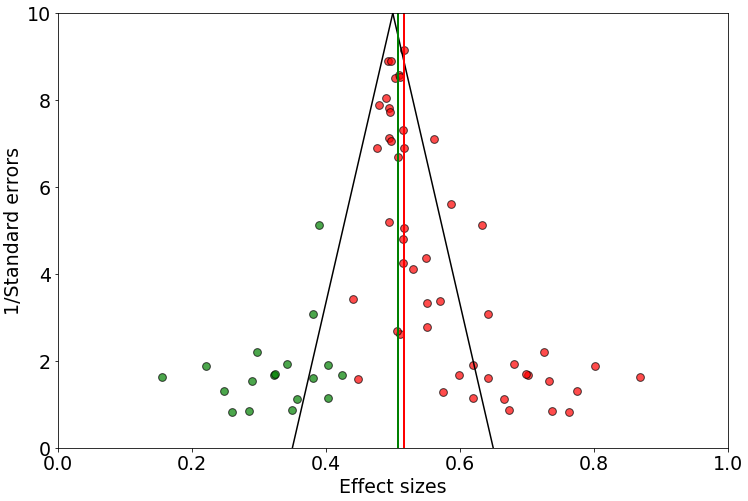
\includegraphics[width=0.6\linewidth]{figures/fig1} 

}

\caption{Funnel plot of simulated data illustrating asymmetry and the trim-and-fill method. The red dots represent the observed studies, the green dots the filled studies. The red and green lines are the fixed-effect pooled ES estimates of the observed studies only and the observed plus the filled studies, respectively.}\label{fig:fig2}
\end{figure}
\vspace{-6mm}

\begin{itemize}
\item
  Begg and Mazumdar's (1994) rank correlation approach is another non-parametric test of funnel plot asymmetry. It involves calculating a normalised version of Kendall's Tau between the deviations of individual ESs from their fixed-effects pooled mean and their sampling variances. This statistic (the normalised Tau) is then tested for significance in reference to the standard normal distribution under the null hypothesis that no association between the effect and variance exists (Vevea et al., 2019).
\item
  Egger's test (Egger, Smith, Schneider, \& Minder, 1997) parametrically checks for funnel plot asymmetry by regressing the ratio of ES to SE on the inverse of SE:
\end{itemize}

\[
\frac{\hat\theta_k}{\hat\sigma_{\hat\theta_k}} = \beta_0 + \beta_1 \frac{1}{\hat\sigma_{\hat\theta_k}}
\tag{6}
\]

\begin{itemize} \item[] Where $\hat\theta_k$ is the ES estimate of the $k$th primary study, $\hat\sigma_{\hat\theta_k}$ is the corresponding SE, and $\beta_0$ and $\beta_1$ are the intercept and the regression coefficient, respectively. The resulting intercept indicates asymmetry if it is significantly larger than zero. This is assumed to occur when, due to bias, small studies with very large ESs are overrepresented, whereas the intercept (the expected scaled ES value as SE goes to infinity) should theoretically equal zero. \end{itemize}

\begin{itemize}
\tightlist
\item
  PET-PEESE (T. Stanley, 2008; T. D. Stanley \& Doucouliagos, 2014) is a more recent method that is gaining in popularity. Similarly to Egger's test, both the precision-effect test (PET) and precision-effect estimate with standard error (PEESE) regress the ES on a proxy of its precision, namely the standard error in the case of PET,
  \[
  \hat\theta_k =  \beta_0 + \beta_1\hat\sigma_{\hat\theta_k}
  \tag{7}
  \]
  and the variance in the case of PEESE.
  \[
  \hat\theta_k =  \beta_0 + \beta_1\hat\sigma_{\hat\theta_k}^2
  \tag{8}
  \]
  However, the theoretical idea motivating this manoeuvre is quite different: here it is assumed that, because the intercept resulting from either one of these two regression analyses represents the ES when the sample variance (or SE) equals zero, this intercept should estimate the true ES.
\end{itemize}

The most prominent \(p\)-value based method is Rosenthal's (1979) Fail-Safe \(N\) method. Its purpose is to compute the number of additional studies reporting non-significant results needed to make the \(p\)-value corresponding to the pooled ES no longer significant. This ``traditional'' procedure remains one of the most widely employed for detecting publication bias despite several explicit recommendations against its use (e.g., Borenstein et al., 2009a; Higgins et al., 2019; Rothstein, Sutton, \& Borenstein, 2005). Due to its many limitations of both mathematical and theoretical nature, the Fail-Safe \(N\) is ``{[}\ldots{]} now generally regarded as valueless'' (Vevea et al., 2019, p. 390).

Two more recent \(p\)-value based methods are the so called \(p\)-curve (Simonsohn, Nelson, \& Simmons, 2014a, 2014b; Simonsohn, Simmons, \& Nelson, 2015) and \(p\)-uniform (van Assen, van Aert, \& Wicherts, 2015). \(p\)-uniform is based on the notion that conditional \(p\)-values are uniformly distributed given a fixed true ES. \(p\)-curve analysis derives its logic from the fact that \(p\)-values are uniformly distributed when the true effect equals zero (the null hypothesis is true), and right skewed when there is a true effect (the null hypothesis is false). Importantly, this also applies to the range of \(p\)-values commonly defined as the region of significance in a given research field, e.g., \((0 < p < 0.05)\) in the behavioural, social, and biomedical sciences. Significant \(p\)-values stemming from a biased pool of studies should, on the contrary, exhibit a left-skewed distribution.

This left skewness is commonly attributed to selective reporting and publishing of effects whose \(p\)-values are over the significance threshold regardless of their magnitude. Such bodies of research are considered to possess little or no \emph{evidential value} (Simonsohn et al., 2014b) as one assumes most of their significant effects to be the product of a combination of \(p\)-hacking\footnote{``trying multiple analyses to obtain statistical significance'' (Simonsohn et al., 2014b, p. 534)} and selective reporting/publication bias. \(p\)-curve analysis therefore involves testing for evidential value in a set of ESs by conducting 6 statistical tests on the subset containing exclusively significant ESs: one binomial test of right skewness, two parametric tests of right skewness, one binomial tests of flatness, and two parametric tests of flatness. There are two parametric tests each as the second one is conducted on half the curve only, i.e., the interval \((0,0.025)\), in order to account for ``ambitious \(p\)-hacking''. The adjusted ES estimate produced by the analysis is, however, based on the full curve.

The last class of publication bias assessment tools, selections models, cannot be exclusively assigned to either category as they are a very versatile methods which allow their user to model \emph{any} process assumed to generate bias in the meta-analytic estimates (Harrer et al., 2021; Vevea et al., 2019). The main purpose of these models is to adjust the observed pooled ES estimate by merging two functions: one describing the distribution of ESs in the absence of bias and the other describing the mechanism by which ESs are assumed to be selected for reporting or publication. Selection models have also been around for decades, although they have enjoyed much less use as they are considerably more complex conceptually and have been barely implemented in commercial point and click software (Vevea et al., 2019).

One relatively simple variety is the three-parameter selection model (McShane et al., 2016), which, as the name suggests, only estimates three parameters: the true average effect \(\mu\), the between-study variance \(\tau^2\), and the likelihood of obtaining non-significant ES in relation to obtaining a significant one, \(\omega_2%
\). What is fixed is the cut-off value \(\alpha_1\), which is usually the significance threshold for a one-sided \(p\)-value, 0.025. The relative likelihood of obtaining a \(p\)-value in this interval (\(0<\alpha_1<0.025\)), \(\omega_1%
\), is set to one. Hence, if the estimated \(\omega_2\) is close to one, the adjusted pooled ES estimate will deviate little from the one based on a standard random-effects model as this would indicate a similar likelihood of obtaining a non-significant ES to obtaining a significant one. Otherwise, the significant ESs will be downweighted if \(\omega_2 < 1\) and upweighted if \(\omega_2 > 1\), which diminishes or augments the pooled ES estimate, respectively.

Fail-Safe \(N\)'s shortcomings were already mentioned. However, this should not be taken to mean that it is the only method with limitations. In fact, Fail-Safe \(N\)'s meaninglessness is one of the very few things the publication bias assessment literature appears to be in agreement about (Carter et al., 2019; Harrer et al., 2021). The methods vary considerably in their assumptions and hence under what conditions they perform well. The different developers of such methods disagree \emph{strongly} about which conditions are realistic in which disciplines and to what degree this should inform the methods' construction. For example, Simonsohn (2017), one of the developers of the \(p\)-curve, deems PET-PEESE to be worse than homoeopathy as it (PET-PEESE) can be actively harmful whereas homoeopathy is simply ineffective. Vevea et al. (2019)\footnote{Vevea being a developer of two selection model varieties (Vevea \& Hedges, 1995; Vevea \& Woods, 2005)}, on the other hand, see the \(p\)-curve and \(p\)-uniform methods as reinventions of the wheel and as ``{[}\ldots{]} modified versions of simplistic early weight-function models'' (p.392). Duval and Tweedie (2000a)\footnote{The developers of the trim-and-fill method, which is widely regarded as being of little use for correcting bias, although potentially useful as a sensitivity analysis (Carter et al., 2019; Hilgard, Engelhardt, \& Rouder, 2017; Moreno et al., 2009; Simonsohn et al., 2014a; van Assen et al., 2015).} quote DuMouchel and Harris (1997) as writing in reference to selection models: ``attempts to assess publication bias beyond simple graphs like the funnel plot seem to involve a tour de force of modeling, and as such are bound to run up against resistance from those who are not statistical modeling wonks'' (p.~95).

Given this intricate state of affairs when it comes to statistical methods of publication bias assessment and correction, it should have become clear that as of yet, there is neither a single method nor a single set of methods which can be recommended as an all-purpose tool (Harrer et al., 2021; Vevea et al., 2019). Simulations studies have shown that no single method outperforms all the others under all conditions (Carter et al., 2019). Another point on which a consensus seems to prevail is that these methods should be used as sensitivity analyses, both with respect to a single method (e.g., by varying the assumptions used) and with respect to which and how many tests one uses (Carter et al., 2019; McShane et al., 2016; Vevea et al., 2019). We are not aware of studies investigating how publication bias is accounted for in tDCS-motor learning research.

\hypertarget{research-questions}{%
\subsection{Research questions}\label{research-questions}}

In sum, 4 principal premises motivated our work: 1. tDCS appears to be remarkably popular as a research tool in basic and clinical research as well as in form of commercial gadgets, 2. meta-analyses of tDCS's effect on motor learning might be substantially impacting research and clinical practice and/or tDCS's uptake as a commercial product, 3. meta-analyses are often of suboptimal methodological quality, which compromises their credibility and informativeness, 4. no methodological evaluation of meta-analyses in tDCS-motor learning research has been conducted as of yet. Our aim was thus to provide such an evaluation while partitioning the concept of methodological quality of a meta-analysis into 3 main aspects:

\begin{enumerate}
\def\labelenumi{\arabic{enumi}.}
\tightlist
\item
  Reporting quality: did the meta-analysis adhere to the PRISMA reporting guidelines? Which items were neglected, if any?
\item
  Reproducibility: how hard is it to reproduce the pooled ES estimate reported in the meta-analysis, if at all, based on the information provided therein? Which necessary pieces of information were missing, if any? If enough information was provided to reproduce the methods, does the reproduced pooled ES equal the reported pooled ES?
\item
  Consideration of publication bias: Did the meta-analysis report attempts to minimise the effects of publication bias? Which statistical or non-statistical methods were used? By conducting a publication bias analysis of our own, do we arrive at the same conclusion regarding the presence of publication bias as the meta-analysts?
\end{enumerate}

Secondary methodological aspects we evaluated included:

\begin{enumerate}
\def\labelenumi{\arabic{enumi}.}
\tightlist
\item
  Had the meta-analysis been pre-registered? If yes, did the pre-registration protocol adhere to meta-analysis pre-registration protocol reporting guidelines PRISMA-P (Moher et al., 2015)? Pre-registering the hypotheses and data analysis plan is essential for distinguishing between confirmatory and exploratory findings (Brian A. Nosek, Ebersole, DeHaven, \& Mellor, 2018). In the context of reviews and meta-analyses, pre-registration protocols ``{[}\ldots{]} act as a guard against arbitrary decision making during review conduct, enable readers to assess for the presence of selective reporting against completed reviews, and, when made publicly available, reduce duplication of efforts and potentially prompt collaboration'' (Shamseer et al., 2015, p. 1).
\item
  Did the meta-analysis discuss outliers? How was the presence of outliers addressed?
  Extreme ES values may affect the validity and robustness of meta-analytic results and there is a general consensus that meta-analyses should examine the presence of outliers and to what extent they influence conclusions (Viechtbauer \& Cheung, 2010).
  \vspace{-6mm}
\end{enumerate}

\hypertarget{methods}{%
\section{Methods}\label{methods}}

Although our methodological approach mostly followed the plan pre-defined in the thesis proposal (accessible on the thesis' Open Science Framework {[}OSF{]} project \href{https://osf.io/uagvf/}{osf.io/uagvf/}), there were important deviations from the plan, especially with respect to reproducibility testing. A document listing these deviations can also be found on the OSF project. For data wrangling, analysis and visualisation, we used \texttt{R} (Version 4.1.2, R Core Team, 2021) and the packages \texttt{dmetar} (Version 0.0.9000, Harrer, Cuijpers, Furukawa, \& Ebert, 2019), \texttt{dplyr} (Version 1.0.7, Wickham, François, Henry, \& Müller, 2021), \texttt{forcats} (Version 0.5.1, Wickham, 2021a), \texttt{ggplot2} (Version 3.3.5, Wickham, 2016), \texttt{MAd} (Version 0.8.2.1, Hoyt, 2014), \texttt{Matrix} (Version 1.3.4, Bates \& Maechler, 2021), \texttt{meta} (Version 5.1.0, Balduzzi, Rücker, \& Schwarzer, 2019), \texttt{metafor} (Version 3.0.2, Viechtbauer, 2010), \texttt{purrr} (Version 0.3.4, Henry \& Wickham, 2020), \texttt{readr} (Version 2.1.0, Wickham \& Hester, 2021), \texttt{readxl} (Version 1.3.1, Wickham \& Bryan, 2019), \texttt{stringr} (Version 1.4.0, Wickham, 2019), \texttt{tibble} (Version 3.1.6, Müller \& Wickham, 2021), and \texttt{tidyr} (Version 1.1.4, Wickham, 2021b).

The package \texttt{renv} (Version 0.14.0, Ushey, RStudio, \& PBC, 2021) was used to ensure long-term reproducibility of our analyses. This thesis was written using RMarkdown and the associated packages \texttt{papaja} (Version 0.1.0.9997, Aust \& Barth, 2020), \texttt{kableExtra} (Version 1.3.4, Zhu, 2021), \texttt{knitr} (Version 1.36, Xie, 2014, 2015, 2021). Both writing and analysis were done using RStudio (Version 2021.9.1.372, RStudio Team, 2021). Data were extracted from figures using WebPlotDigitizer (\href{https://apps.automeris.io/wpd/}{apps.automeris.io/wpd/}, Rohatgi, 2021). A video demonstration of how we extracted data from figures is available on the OSF project.

\hypertarget{sample-of-meta-analyses}{%
\subsection{Sample of meta-analyses}\label{sample-of-meta-analyses}}

Three meta-analyses (Hung et al., 2021b; Kang, Summers, \& Cauraugh, 2016; Kang, Weingart, \& Cauraugh, 2018) were selected based on the following eligibility criteria:

\begin{itemize}
\tightlist
\item
  Meta-analysis studies which quantitatively synthesise multiple (at least 3) primary studies on the effects of tDCS on motor learning.
\item
  No restriction on primary outcomes (e.g., how speed or accuracy were measured), designs of primary studies (e.g., randomised vs.~crossover designs), or participants (e.g., clinical or healthy subjects) in the primary studies were imposed.
\end{itemize}

Exclusion criteria:

\begin{itemize}
\tightlist
\item
  Reviews of any type without a quantitative synthesis
\item
  Primary studies
\item
  Reviews which did not report a ``main'' meta-analysis, but rather multiple meta-analyses of subgroups of studies.
\end{itemize}

All three meta-analyses were found via quick, non-systematic Google Scholar or Web of Science searches.

\hypertarget{data-extraction}{%
\subsection{Data extraction}\label{data-extraction}}

\hypertarget{elements-extracted}{%
\subsubsection{Elements extracted}\label{elements-extracted}}

There were two types of elements extracted:

\begin{enumerate}
\def\labelenumi{\arabic{enumi}.}
\tightlist
\item
  Primary study level variables (e.g., sample sizes, means and SDs), were extracted from both the primary studies and the meta-analyses.
\item
  Meta-analysis level variables (e.g., pooled SMD, publication bias control related variables).
\end{enumerate}

Both data sheets are also available on the OSF project page. They can be found by navigating to the GitHub thesis branch in the folder ``data\_thesis'' under the names ``Data\_ps\_raw'' and ``Data\_ma\_raw'', respectively. The codebook explaining column headers in the data sheets is also accessible on the OSF project (folder ``Post\_data\_extraction'').

\hypertarget{data-extraction-procedure}{%
\subsubsection{Data extraction procedure}\label{data-extraction-procedure}}

Data for all non-reproducibility-related variables were extracted directly to Google Sheets (no specialised data extraction software was used). The data extraction procedure for the purpose of testing reproducibility differed substantially from the rest and is described below.

\hypertarget{procedure-coding-and-data-analysis}{%
\subsection{Procedure, coding, and data analysis}\label{procedure-coding-and-data-analysis}}

\hypertarget{reporting-quality-1}{%
\subsubsection{Reporting quality}\label{reporting-quality-1}}

The adherence of each meta-analysis to the PRISMA reporting guidelines (Liberati et al., 2009; Moher et al., 2009) were checked. Concretely, for each of the 27 PRISMA items, we coded whether the meta-analysis reported the relevant information as recommended, regardless of whether the meta-analysis reported having adhered to any reporting guidelines. Besides coding whether the meta-analysis had been pre-registered, we checked whether the pre-registration protocol adhered to the PRISMA-P reporting guidelines (Moher et al., 2015; Shamseer et al., 2015) for such protocols, provided that the meta-analysis had been pre-registered and published later than 2015.

\hypertarget{reproducibility-1}{%
\subsubsection{Reproducibility}\label{reproducibility-1}}

We based our treatment of meta-analysis reproducibility on the definition and principles of reproducibility put forward by the American Statistical Association (Broman et al., 2017): a meta-analysis is reproducible if its authors provided enough information to go through all the necessary procedures (search, screening, data extraction, calculation of primary ESs, calculation of the pooled ES\ldots) to arrive at the same results. However, although we acknowledge the importance of all these steps, we, like Gøtzsche et al.~(2007), Lakens et al.~(2017), and Maassen et al.~(2020), focused on data extraction and calculation of ES estimates.

Since reproducing the primary ESs is a necessary step towards reproducing the pooled SMD, we constructed a scheme for classifying their reproducibility status. The two variables in this scheme are A. whether the primary ES could be successfully reproduced or approximated numerically\footnote{An ES estimate was considered successfully reproduced (or reproducible) if the reproduced ES equalled the one reported in the meta-analysis at the second decimal (e.g., 0.3324543 = 0.33) and approximated if the reproduced ES equalled the reported one at the first decimal (e.g., 0.1767492 \(\approx\) 0.22).} (results reproducibility) and B. whether the procedure we followed in reproducing the ES strictly corresponded to the information given in the meta-analysis or to the procedure apparently adopted for at least two other ESs included in the meta-analysis (methods reproducibility).

Table 4 depicts the classification system in which we use SMD (for standardised mean difference) instead of ES since SMD was the only measure of ES employed in the meta-analyses we evaluated. ``Procedure'' here includes such analytic decisions as using \(p\)-values or test statistics in combination with sample sizes to estimate the SMD for a given primary study, using the raw means and SDs instead of means and SDs of changes in the outcome from baseline or vice versa, using follow-up means and SDs instead of post means and SDs, etc.. The second variable in the classification system was thus mainly adopted to capture cases where there was a discrepancy between how the meta-analysts reported having computed a primary ES and how they actually computed it.

\singlespacing
\begingroup\fontsize{10}{12}\selectfont

\begin{longtable}[t]{>{\raggedright\arraybackslash}p{18em}>{\raggedright\arraybackslash}p{12em}>{\raggedright\arraybackslash}p{12em}}
\caption{\label{tab:table4}Reproducibility classification scheme.}\\
\toprule
. & Reproduced SMD equalled or approximated reported SMD & Reproduced SMD neither equalled nor approximated reported SMD\\
\midrule
Strictly following information given in the meta-analysis or a standard procedure apparently adopted for at least two other successfully reproduced SMDs & 1. Faithfully reproducible SMD & 2. Faithfully irreproducible SMD\\
\midrule
Following a procedure which either does not entirely correspond to the procedure the meta-analysts report having adopted OR does not (necessarily) produce an SMD that is comparable to what would result from following the procedure apparently adopted for at least two other successfully reproduced SMDs & 3. Brute-force reproducible SMD & 4. Brute-force irreproducible SMD\\
\bottomrule
\end{longtable}
\endgroup{}
\doublespacing

It is important to re-emphasise our distinction between ``reproduced'' and ``reproducible''. ``Reproduced'' simply means we calculated something and compared it with the original, whereas ``reproducible'' SMDs were those which were successfully reproduced computationally. Thus, ``faithfully'' and ``brute-force'' refer to whether we found data in the corresponding primary study that could be used at all and ``reproducible'' and ``irreproducible'' to whether the SMD resulting from our calculation matches (or approximates) the original. In other words, if a given SMD is methodologically irreproducible given the data reported in the primary study, then its faithful reproducibility cannot be tested and would have to be excluded when calculating the pooled SMD (see information about the different meta-analytic models we fit below). Furthermore, if we classify an SMD as ``faithfully irreproducible'', this does not imply that it is necessarily also brute-force irreproducible because in most cases, we did not collect further values to test brute-force reproducibility if the values we chose to test faithful reproducibility very clearly corresponded to the meta-analysts' description of their procedure.

Reproducibility testing was an iterative process which involved several rounds of data extraction. The initial round of data extraction and testing reproducibility did not yield a lot of reproducible SMDs as most primary studies did not report the values necessary to directly compute an SMD and/or its sampling variance (e.g., for a between groups Cohen's \(d\) this would be the group means, SDs and sample sizes). Therefore, a less strict data extraction procedure was adopted, which involved the following steps:

\begin{enumerate}
\def\labelenumi{\arabic{enumi}.}
\tightlist
\item
  For each primary SMD, we first looked for the raw means and SDs of the outcome reported as having been used by the meta-analysts. If the primary study reported multiple sets of means and SDs which can be seen as corresponding to the outcome described in the meta-analysts (e.g., the outcome in the meta-analysis for a given primary study is ``Fugl-Myer Test'' but the primary study reports values for ``Fugl-Myer Test - upper limbs'' and ``Fugl-Myer Test - full''), all sets were extracted.
\item
  If no means and SDs for the relevant outcome were reported in the primary study, means and SDs were extracted from figures. If no figures were reported which contained means and SDs (or SEs or confidence intervals {[}CIs{]}), \(p\) and/or \(t\)-values for tests on the relevant outcome were extracted, which in combination with \(n\)s can be converted to SMDs.
\item
  Based on all extracted values, we computed each primary SMD using the estimator (Cohen's \(d\) or Hedges' \(g\)) reported as having been used by the meta-analysts. If this information was not given in the meta-analysis, we tried both formulas and for further analysis used the one which consistently approximated the reported SMDs better.
\item
  If none of the values extracted reproduced a given SMD, we double checked the correctness of the data extracted and, in some cases, extracted more values from the primary study (à la brute-force) and computed the SMD based on those.
\item
  We computed the sampling variances based on the SMDs and the corresponding \(n\)s.
\item
  For each meta-analysis, we fit three meta-analytic models (MAMs): 1. Based on the faithfully reproduced SMDs. 2. Based on the faithfully reproduced SMDs plus brute-force reproduced. 3. Based on the SMDs and sampling variances reported in the meta-analysis\footnote{Sampling variances were not reported in any of the three meta-analyses. They were calculated based on SEs extracted from funnel plots in the case of the first two meta-analyses and based on CIs for the third meta-analysis}. This was done to test for analytical reproducibility of the pooled SMD and to find out which between-study heterogeneity estimator was used.
\end{enumerate}

The concrete procedure for data extraction thus differed for each single primary study. A detailed description of all values we extracted and how we analysed them is provided in the data analysis notebook, also available on our OSF project page.

\hypertarget{publication-bias-control-1}{%
\subsubsection{Publication bias control}\label{publication-bias-control-1}}

The non-statistical approaches to accounting for publication bias that we coded were:

\begin{enumerate}
\def\labelenumi{\arabic{enumi}.}
\tightlist
\item
  Searched clinical trial registries (e.g., ClinicalTrials.org)
\item
  Searched thesis and dissertation repositories (e.g., ProQuest)
\item
  Did not restrict their search to studies written in English
\item
  Contacted known researchers in the field to inquire about unpublished results
\item
  Contacted authors of included studies to ask for raw data or unpublished results
\end{enumerate}

Besides coding whether any statistical methods were used at all and which, we tested for publication bias in each meta-analysis using 3 different methods: PET-PEESE (T. Stanley, 2008; T. D. Stanley \& Doucouliagos, 2014), \(p\)-curve (Simonsohn et al., 2014a, 2014b), and the three-parameter selection model (McShane et al., 2016). For each meta-analysis, we concluded that publication bias is a concern in the studies synthesised if at least two out of the three methods used yielded results indicating the presence of publication bias. Although such a ``majority vote'' approach is not recommended for actual publication bias assessment (Carter et al., 2019, p. 140), we adopted it so as to have an unambiguous decision rule whether our analysis agrees with that of the meta-analysts or not. For these analyses, we used the SMDs and the sample sizes reported in the meta-analyses along with the sampling variances extracted from the funnel plots in the case of the first two meta-analyses and calculated based on the CIs in the case of the third meta-analysis.

\hypertarget{outlierinfluential-study-analysis}{%
\subsubsection{Outlier/influential study analysis}\label{outlierinfluential-study-analysis}}

Besides coding whether each meta-analysis checked for the existence of outliers among the included studies and how this was done, we tested this ourselves for each meta-analysis using the leave-one-out method (Harrer et al., 2021; Tobias, 1999).

\hypertarget{results}{%
\section{Results}\label{results}}

\hypertarget{general-description-of-the-meta-analyses}{%
\subsection{General description of the meta-analyses}\label{general-description-of-the-meta-analyses}}

Table 5 gives an overview of the three meta-analyses we reviewed. Meta-analyses 1 and 2 aimed to estimate the effectiveness of tDCS for improving motor function in post-stroke patients, although meta-analysis 2 focused exclusively on the effects of cathodal tDCS. Meta-analysis 3 investigated effectiveness of tDCS for improving surgical performance of surgery trainees. Meta-analyses 2 and 3 reported more primary SMDs than primary studies because they drew two comparisons from some primary studies. In meta-analysis 1, the double comparisons represented cathodal vs.~sham and anodal vs.~sham pairs, whereas in meta-analysis 2 comparison pairs were based on two different outcomes. The first meta-analysis synthesised the results of 13 randomised controlled trials (RCTs) and 4 crossover trials, the second 6 RCTs and 9 crossover trials, the third 5 RCTs and one crossover trial. None of the three meta-analyses had been pre-registered. According to Google Scholar, the meta-analyses were cited 197, 12, and two times, respectively, as of 16.11.2021. The average total sample size \(N\) of the primary studies included in the three meta-analyses, that is, mean of \(n_t + n_c\), were \textasciitilde{} 26, \textasciitilde{} 24, and \textasciitilde{} 32, respectively.

\singlespacing
\begingroup\fontsize{11}{13}\selectfont

\begin{longtable}[t]{ccccc}
\caption{\label{tab:table5}Reviewed meta-analyses.}\\
\toprule
Meta-analysis ID & Authors & Year & Number of studies & Number of SMDs\\
\midrule
1 & Kang, Summers, \& Cauraugh & 2016 & 17 & 21\\
2 & Kang, Weingart, \& Cauraugh & 2018 & 15 & 20\\
3 & Hung et al. & 2021 & 6 & 6\\
\bottomrule
\end{longtable}
\endgroup{}
\doublespacing

\hypertarget{reporting-quality-2}{%
\subsection{Reporting quality}\label{reporting-quality-2}}

Meta-analyses 1 did not report having adhered to any reporting guidelines. Despite this, it can be seen as having reported the content of 18 out of the 27 PRISMA (Moher et al., 2009) items. Meta-analysis 2 mentioned PRISMA and adhered to 19 out of the 27 items. Meta-analysis 3 reported having adhered to the most recent PRISMA guidelines (Page, McKenzie, et al., 2021) but we evaluated the adherence to the items of the 2009 version to ensure comparability to the other meta-analyses. Meta-analysis reported the content of 25 out of the 27 items. Table 6 summarises the three meta-analyses' adherence to the PRISMA items.

\singlespacing
\begingroup\fontsize{10}{12}\selectfont

\begin{longtable}[t]{>{\raggedleft\arraybackslash}p{5em}>{\raggedright\arraybackslash}p{15em}>{\raggedright\arraybackslash}p{7em}>{\raggedright\arraybackslash}p{7em}>{\raggedright\arraybackslash}p{7em}}
\caption{\label{tab:table6}PRISMA items adherence of the three meta-analyses}\\
\toprule
Item number & Original item label & 1 & 2 & 3\\
\midrule
\endfirsthead
\caption[]{\label{tab:table6}PRISMA items adherence of the three meta-analyses \textit{(continued)}}\\
\toprule
Item number & Original item label & 1 & 2 & 3\\
\midrule
\endhead
\midrule
\multicolumn{5}{r@{}}{}\
\endfoot
\bottomrule
\endlastfoot
1 & Title & Reported & Reported & Reported\\
2 & Structured Summary & Not reported & Reported & Not reported\\
3 & Rationale & Reported & Reported & Reported\\
4 & Objectives & Not reported & Reported & Reported\\
5 & Protocol and registration & Not reported & Not reported & Reported\\
6 & Eligibility criteria & Reported & Reported & Reported\\
7 & Information sources & Reported & Reported & Reported\\
8 & Search & Not reported & Not reported & Reported\\
9 & Study selection & Not reported & Not reported & Not reported\\
10 & Data collection process & Not reported & Not reported & Reported\\
11 & Data items & Reported & Reported & Reported\\
12 & Risk of bias in individual studies & Not reported & Reported & Reported\\
13 & Summary measures & Reported & Reported & Reported\\
14 & Synthesis of results & Reported & Reported & Reported\\
15 & Risk of bias across studies & Reported & Reported & Reported\\
16 & Additional analyses & Reported & Reported & Reported\\
17 & Study selection & Reported & Reported & Reported\\
18 & Study characteristics & Reported & Reported & Reported\\
19 & Risk of bias within studies & Not reported & Reported & Reported\\
20 & Results of individual studies & Reported & Reported & Reported\\
21 & Synthesis of results & Reported & Reported & Reported\\
22 & Risk of bias across studies & Reported & Reported & Reported\\
23 & Additional analysis & Reported & Reported & Reported\\
24 & Summary of evidence & Reported & Reported & Reported\\
25 & Limitations & Not reported & Not reported & Reported\\
26 & Condusions & Reported & Reported & Reported\\
27 & Funding & Reported & Not reported & Reported\\*
\end{longtable}

Reported \& Not reported \& Reported\textbackslash*
\textbackslash end\{longtable\}
\endgroup{}
\vspace{-8mm}

\begin{tablenotes}[para,flushleft]
      \small
      \item \textit{Note.} Meta-analysis 3 indicated that it had not been pre-registered.
    \end{tablenotes}
\doublespacing

A more detailed description of the extent to which the three meta-analyses adhered to items 6 to 9 and 17 is provided in Table 7. All three meta-analyses adequately described their eligibility criteria but none of them described the actual process of how the criteria were enforced. All three meta-analyses did report the result of this process.

\singlespacing
\begingroup\fontsize{10}{12}\selectfont

\begin{longtable}[t]{>{\raggedleft\arraybackslash}p{4em}>{\raggedright\arraybackslash}p{7em}>{\raggedright\arraybackslash}p{10em}>{\raggedright\arraybackslash}p{10em}>{\raggedright\arraybackslash}p{10em}}
\caption{\label{tab:table7}Detailed description of adherence to PRISMA items 6-9 and 17}\\
\toprule
Item number & Original item label & 1 & 2 & 3\\
\midrule
\endfirsthead
\caption[]{\label{tab:table7}Detailed description of adherence to PRISMA items 6-9 and 17 \textit{(continued)}}\\
\toprule
Item number & Original item label & 1 & 2 & 3\\
\midrule
\endhead
\midrule
\multicolumn{5}{r@{}}{}\
\endfoot
\bottomrule
\endlastfoot
6 & Eligibility criteria & Target study characteristics as well as inclusion and exclusion criteria described but not following the PICO scheme (e.g., nothing about the outcomes). Rational unclear “Our literature search concentrated on tDCS studies that investigated long-term effects on motor functions post-stroke.”. & Target study characteristics as well as inclusion and exclusion criteria described but not following the PICO scheme (e.g., nothing about the outcomes). Rational unclear. & Target study characteristics as well as inclusion and exclusion criteria described following the PICO scheme but no actual outcomes were mentioned (only "change in surgical performance". Rational unclear.\\
7 & Information sources & Databases used for “initial” search were listed. No mention of whether authors of primary authors were contacted. Dates of coverage described. & Databases used were listed. No mention of whether authors of primary authors were contacted. Dates of coverage described. & Databases used were listed. The meta-analysts mention in the appendix having contacted the authors of primary studies regarding data but not how the authors resonded. Dates of coverage described.\\
8 & Search & Although the meta-analysts listed the search keywords used, they did not a describe a full search strategy for any of the databases. & Although the meta-analysts listed the search keywords used, they did not a describe a full search strategy for any of the databases. & The meta-analysts listed both the search keywords used and the full search strategy for PubMed and other databases.\\
9 & Study selection & The meta-analysts did not describe how the different authors contributed to the different stages of eligibility checking or how potential disagreements were resolved. & The meta-analysts did not describe how the different authors contributed to the different stages of eligibility checking or how potential disagreements were resolved. & The meta-analysts did not describe how the different authors contributed to the different stages of eligibility checking or how potential disagreements were resolved.\\
17 & Study selection & The meta-analysts reported how many studies were initially included and how many were subsequently excluded (including reasons). No PRISMA flow chart was provided. & The meta-analysts reported how many studies were initially included and how many were subsequently excluded in a PRISMA flow chart (including reasons). & The meta-analysts reported how many studies were initially included and how many were subsequently excluded in a PRISMA flow chart (including reasons).\\*
\end{longtable}

ction \& The meta-analysts reported how many studies were initially included and how many were subsequently excluded (including reasons). No PRISMA flow chart was provided. \& The meta-analysts reported how many studies were initially included and how many were subsequently excluded in a PRISMA flow chart (including reasons). \& The meta-analysts reported how many studies were initially included and how many were subsequently excluded in a PRISMA flow chart (including reasons).\textbackslash*
\textbackslash end\{longtable\}
\endgroup{}
\doublespacing

\hypertarget{reproducibility-2}{%
\subsection{Reproducibility}\label{reproducibility-2}}

We faced difficulties in reproducing the primary SMDs and their sampling variances for all three meta-analyses, mainly due to limited reporting of the methods sections. None of the three meta-analyses shared their data or provided data analysis code. Although meta-analysis 3 stated that data ``was available upon reasonable request'' (p.~11), the corresponding author of the meta-analysis did not respond to our email requesting more information/data. The process necessitated several time-consuming rounds of data extraction and testing. Which relevant pieces of information were missing and how many primary SMDs could be successfully reproduced is reported below for each meta-analysis separately. The effect of irreproducible primary SMDs on the pooled SMDs is also reported. Since all three meta-analyses reported having fit a random-effects model using the Comprehensive Meta-Analysis software\footnote{In the case of the first meta-analysis, we were informed by the first author of the meta-analysis that they used the Comprehensive Meta-Analysis software in response to an email asking for further information. Our email's text as well as all the reproducibility-relevant information contained in the meta-analysts' response (not the actual text of their responses) can be found in the document ``Email\_to\_authors'' on our OSF project.}, which per default estimates between-study heterogeneity via the Der-Simonian-Laird method (DerSimonian \& Laird, 1986), we used these settings for all our analyses, too.

\hypertarget{meta-analysis-1}{%
\subsubsection{Meta-analysis 1}\label{meta-analysis-1}}

The authors of this meta-analysis reported the following reproducibility-relevant information/data:

\begin{itemize}
\tightlist
\item
  Standardised ES measure is SMD
\item
  Group sample sizes for each primary SMD calculated. In case of crossover studies, they reported the total sample size for both the control and treatment groups.
\item
  All primary SMDs calculated
\item
  CI lower and upper limits for each SMD
\item
  The outcome measure for each SMD (e.g., ``Total latency score in JHFT'')
\item
  What the two compared groups represented (e.g., control group: ``sham before inpatient daily rehabilitation at retention'', treatment group: ``ctDCS on cH before inpatient daily
  rehabilitation at retention'')
\item
  random-effects model
\item
  The pooled SMD
\end{itemize}

The following information was missing:

\begin{itemize}
\tightlist
\item
  Type of SMD used (Cohen's \(d\) vs.~Hedge's \(g\))
\item
  Whether a different method of standardisation was used for the crossover studies (since there are no two groups whose SDs can be pooled to standardise the mean difference)
\item
  Sampling variances of the SMDs (they had to be extracted from the funnel plot)
\item
  Whether sampling variances were calculated differently for the SMDs corresponding to crossover trials
\item
  Which type of values were used to compute each SMD (e.g., means and SDs vs.~\(p\)-value and \(n\)s)
\item
  Which exact values were used and where they were found (e.g., \(p\)-value reported on page \(x\) line \(y\) or means and SDs reported in Figure \(z\))
\item
  Rationale for choosing outcomes
\item
  Enough details about the outcome used so as to leave no room for ambivalence (e.g., ``Upper Limb FMA'' instead of just ``FMA'' when the primary study reported both ``Upper Limb FMA'' and ``Total )
\item
  Which between-study heterogeneity estimator was used
\item
  Software used to run the meta-analysis
\end{itemize}

Table 7 summarises the reproducibility status and classification of each primary SMD. Six SMDs were successfully reproduced following the procedure as described in the meta-analysis or the seemingly standard procedure. Five further SMDs were approximated. Following a deviating procedure, three more SMDs could be reproduced.

\singlespacing
\begingroup\fontsize{9.7}{11.7}\selectfont

\begin{longtable}[t]{>{\raggedright\arraybackslash}p{3em}>{\raggedright\arraybackslash}p{5em}>{\raggedright\arraybackslash}p{5em}>{\raggedright\arraybackslash}p{12em}>{\raggedright\arraybackslash}p{16em}}
\caption{\label{tab:table8}Reproducibility of primary SMDs, Meta-analysis 1}\\
\toprule
SMD no. & Reported SMD & Reproduced SMD & Reproducibility classification & Reason for irreproducibility\\
\midrule
1 & 0.16 & 0.16 & Faithfully reproducible & Not applicable.\\
2 & 0.18 & 0.17 & Faithfully reproducible & Not applicable.\\
3 & 0.36 & 0.36 & Faithfully reproducible & Not applicable.\\
4 & 0.08 & 0.12 & Faithfully reproducible & Not applicable.\\
5 & 0.38 & 0.38 & Faithfully reproducible & Not applicable.\\
6 & 0.04 & 0.04 & Faithfully reproducible & Not applicable.\\
7 & 0.06 & 0.06 & Faithfully reproducible & Not applicable.\\
8 & 1.59 & 1.68 & Faithfully irreproducible & Not \vphantom{1} inferable.\\
9 & 1.08 & 1.15 & Faithfully irreproducible & Not inferable.\\
10 & 1.05 & 1.02 & Faithfully reproducible & Not applicable.\\
11 & 1.39 & 1.35 & Faithfully reproducible & Not applicable.\\
12 & 0.93 & NA & Brute-force
irreproducible & Not inferable.\\
13 & 0.82 & NA & Brute-force
irreproducible & Not inferable.\\
14 & 0.29 & 0.29 & Faithfully reproducible & Not applicable.\\
15 & 0.61 & 0.64 & Faithfully reproducible & Not applicable.\\
16 & 1.43 & 0.18 & Faithfully irreproducible, Brute-force reproducible & Outcome used does not correspond to description.\\
17 & 0.94 & 0.18 & Faithfully irreproducible & Not inferable.\\
18 & 0.24 & 0.54 & Faithfully irreproducible & Not inferable.\\
19 & 0.65 & NA & Brute-force reproducible & Outcome used does not correspond to description.\\
20 & 0.72 & NA & Brute-force reproducible & Sucessfully reproduced using a p-value derived from a medians test.\\
21 & 0.53 & 1.61 & Faithfully irreproducible & Not inferable.\\
\bottomrule
\end{longtable}
\endgroup{}
\vspace{-8mm}
\begin{tablenotes}[para,flushleft]
      \small
      \item \textit{Note.} The "Reproduced SMD" column lists the faithfully reproduced SMDs only (rounded to the second decimal).
    \end{tablenotes}
\doublespacing

Using the SMDs and the sample sizes reported in the meta-analysis along with the sampling variances extracted from the funnel plot (MAM 3), all meta-analytic estimates were successfully reproduced. This MAM was thus treated as the ``reported'' variety and compared to the two other MAMs. All three MAMs are depicted as forest plots in Figure 3. The pooled SMDs from MAMs 1 and 2 deviate from the reported pooled SMD by 0.05 and 0.11 SDs, respectively. More noteworthy differences are observable in the heterogeneity estimates \(I^2\) and \(\tau^2\).

\begin{figure}[H]

{\centering \subfloat[MAM 1, based on faithfully reproduced SMDs.\label{fig:fig3-1}]{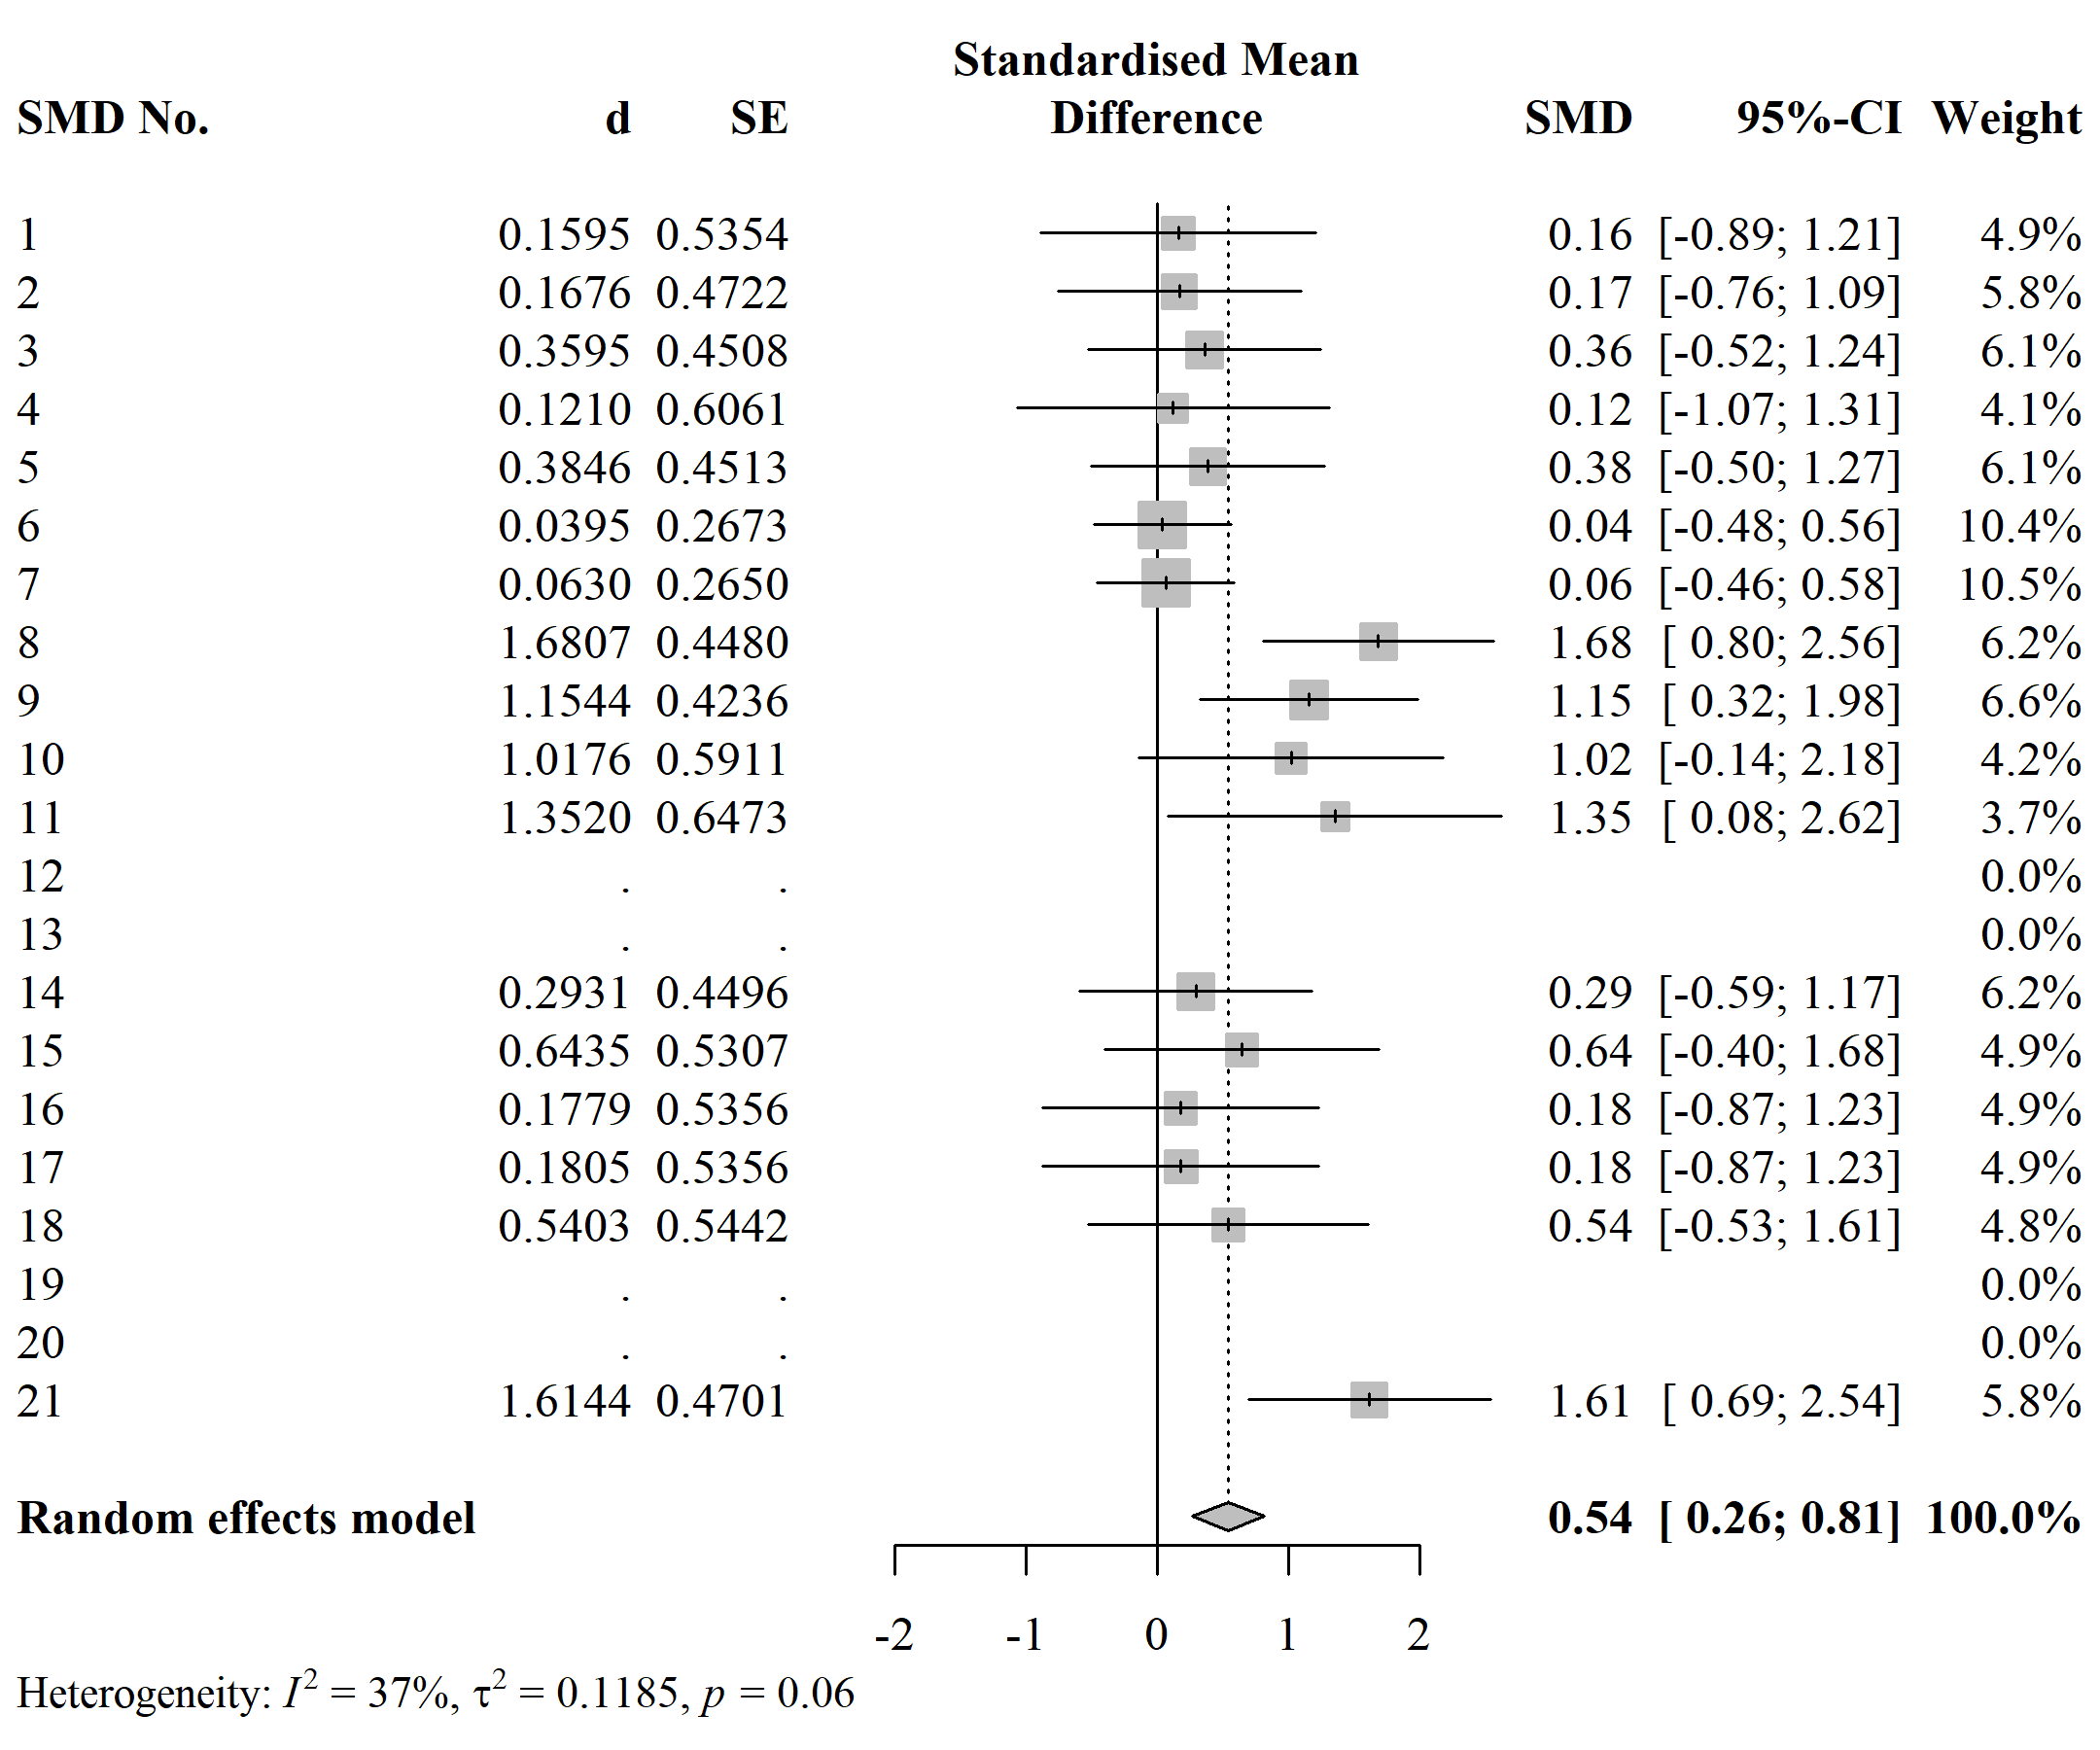
\includegraphics[width=0.5\linewidth]{figures/fig3_mam1} }\subfloat[MAM 2, based on faithfully and brute-force reproduced SMDs.\label{fig:fig3-2}]{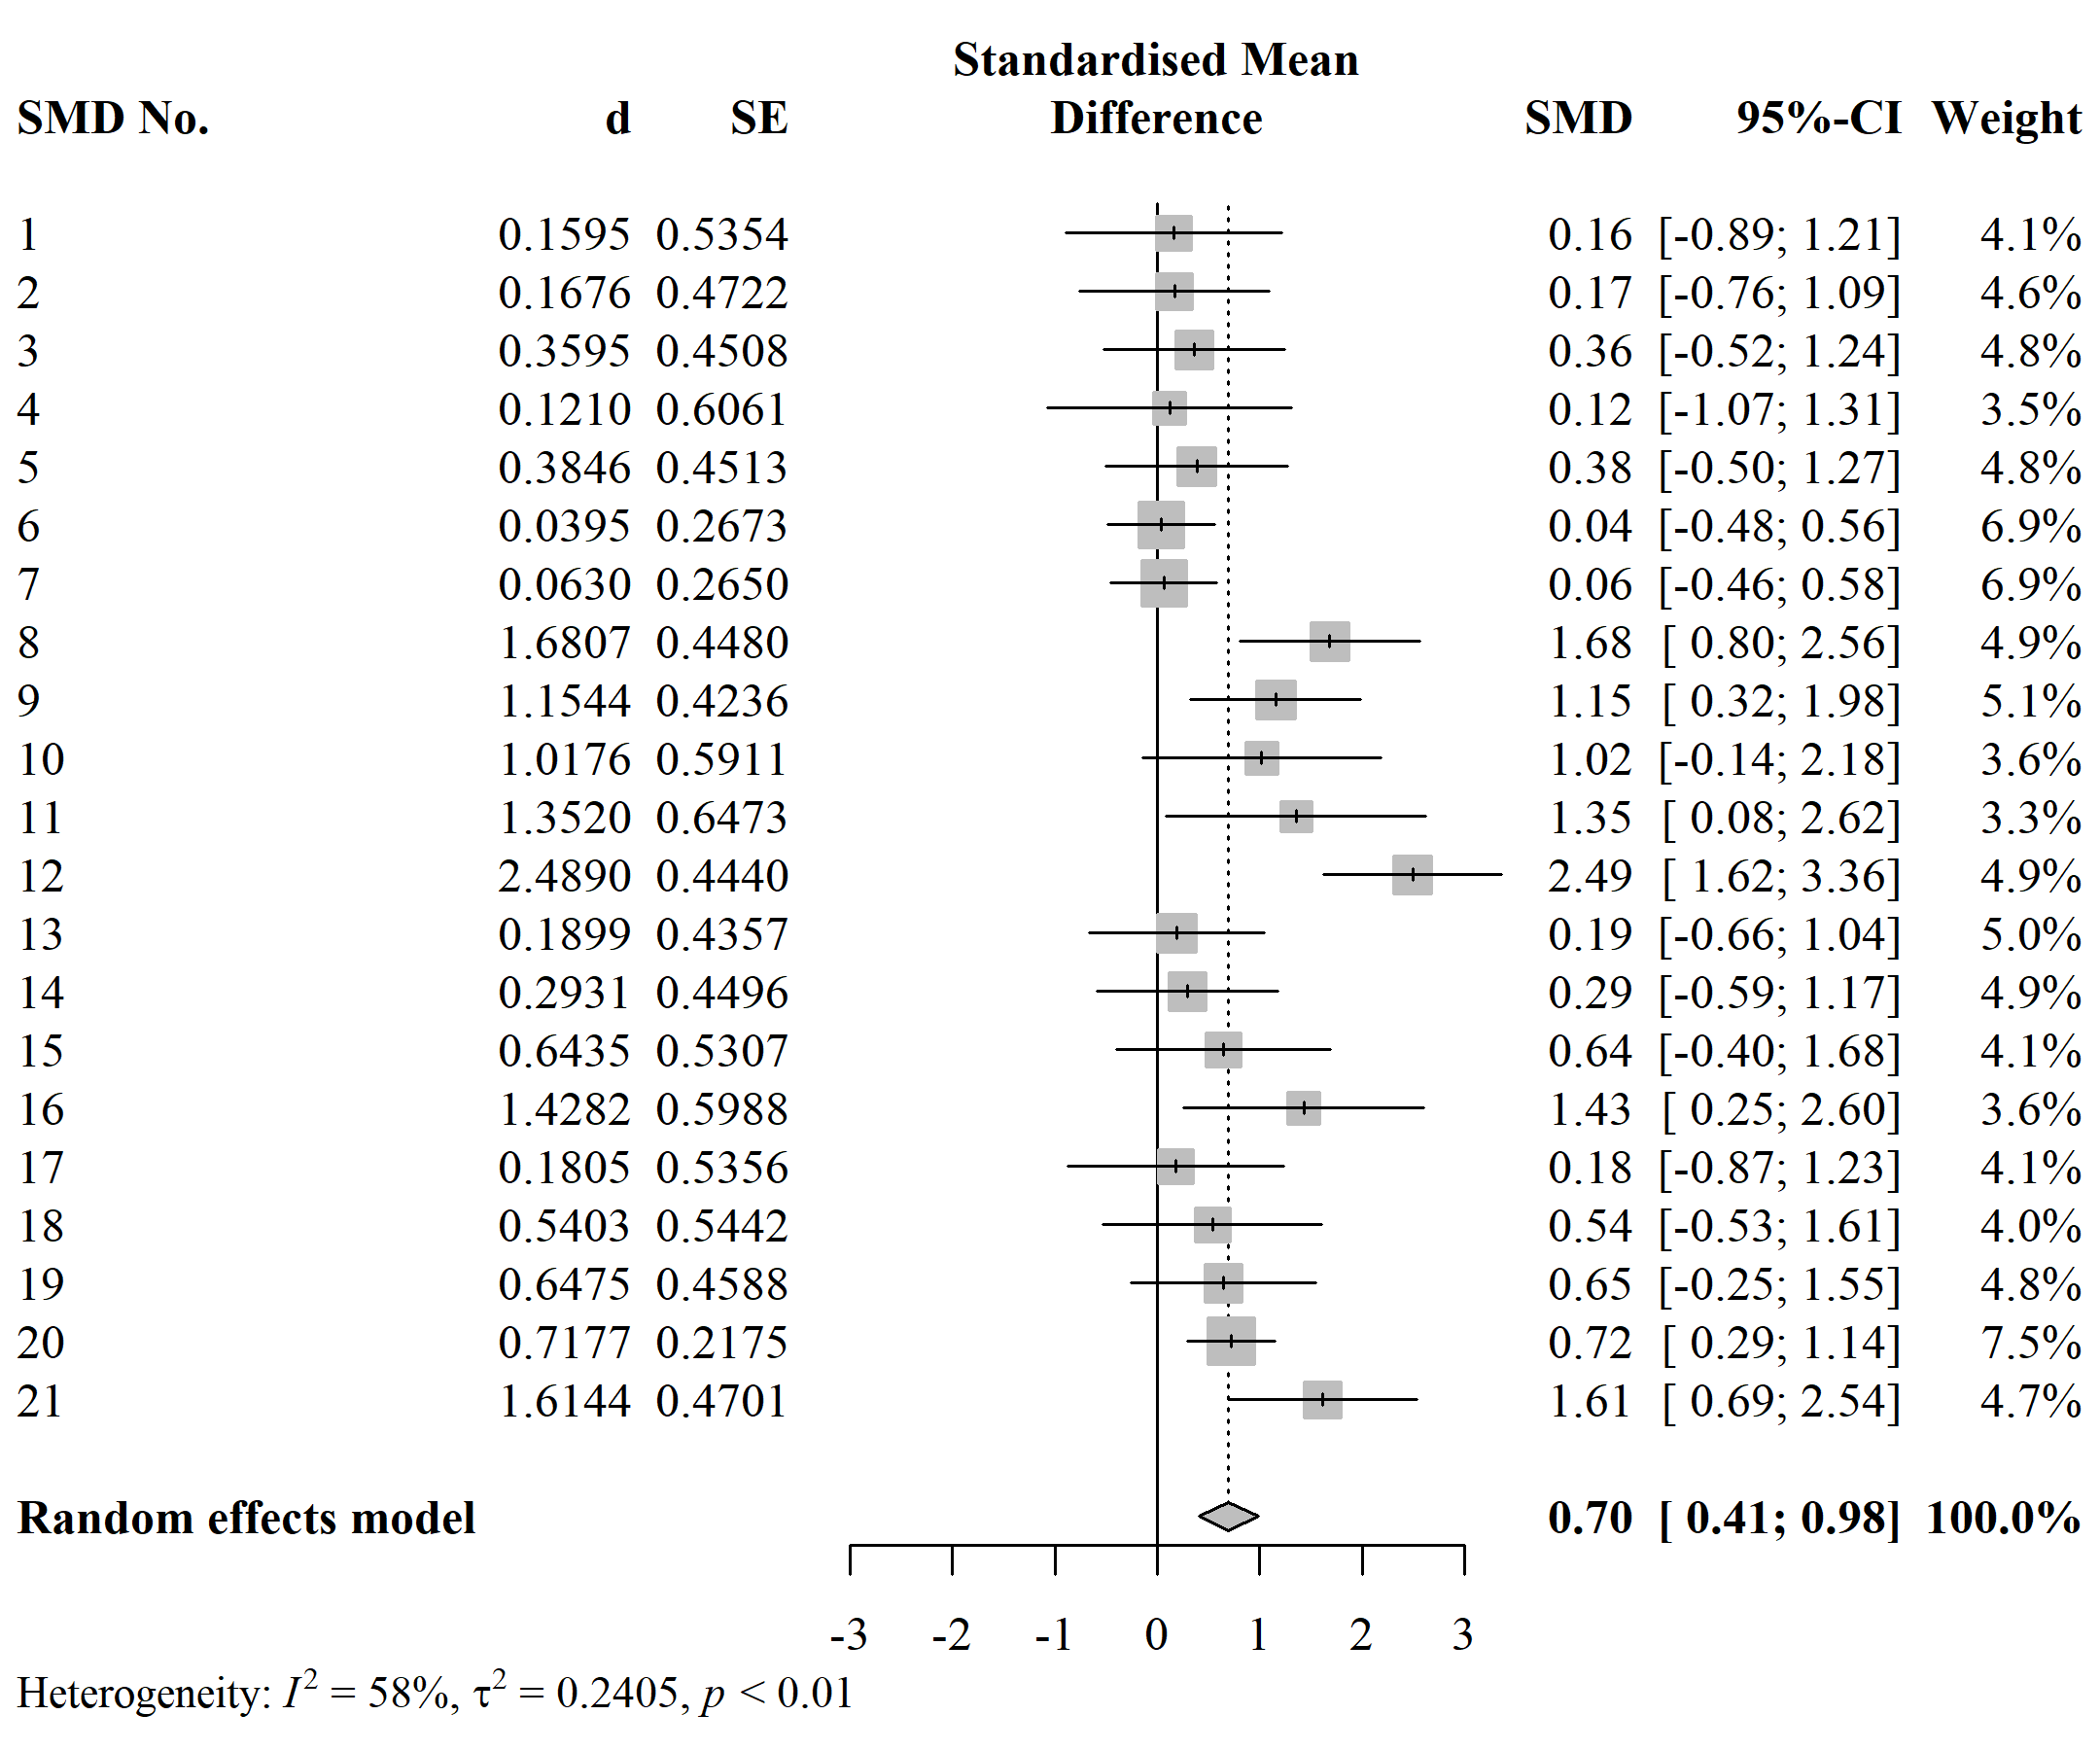
\includegraphics[width=0.5\linewidth]{figures/fig3_mam2} }\newline\subfloat[MAM 3, based on reported SMDs.\label{fig:fig3-3}]{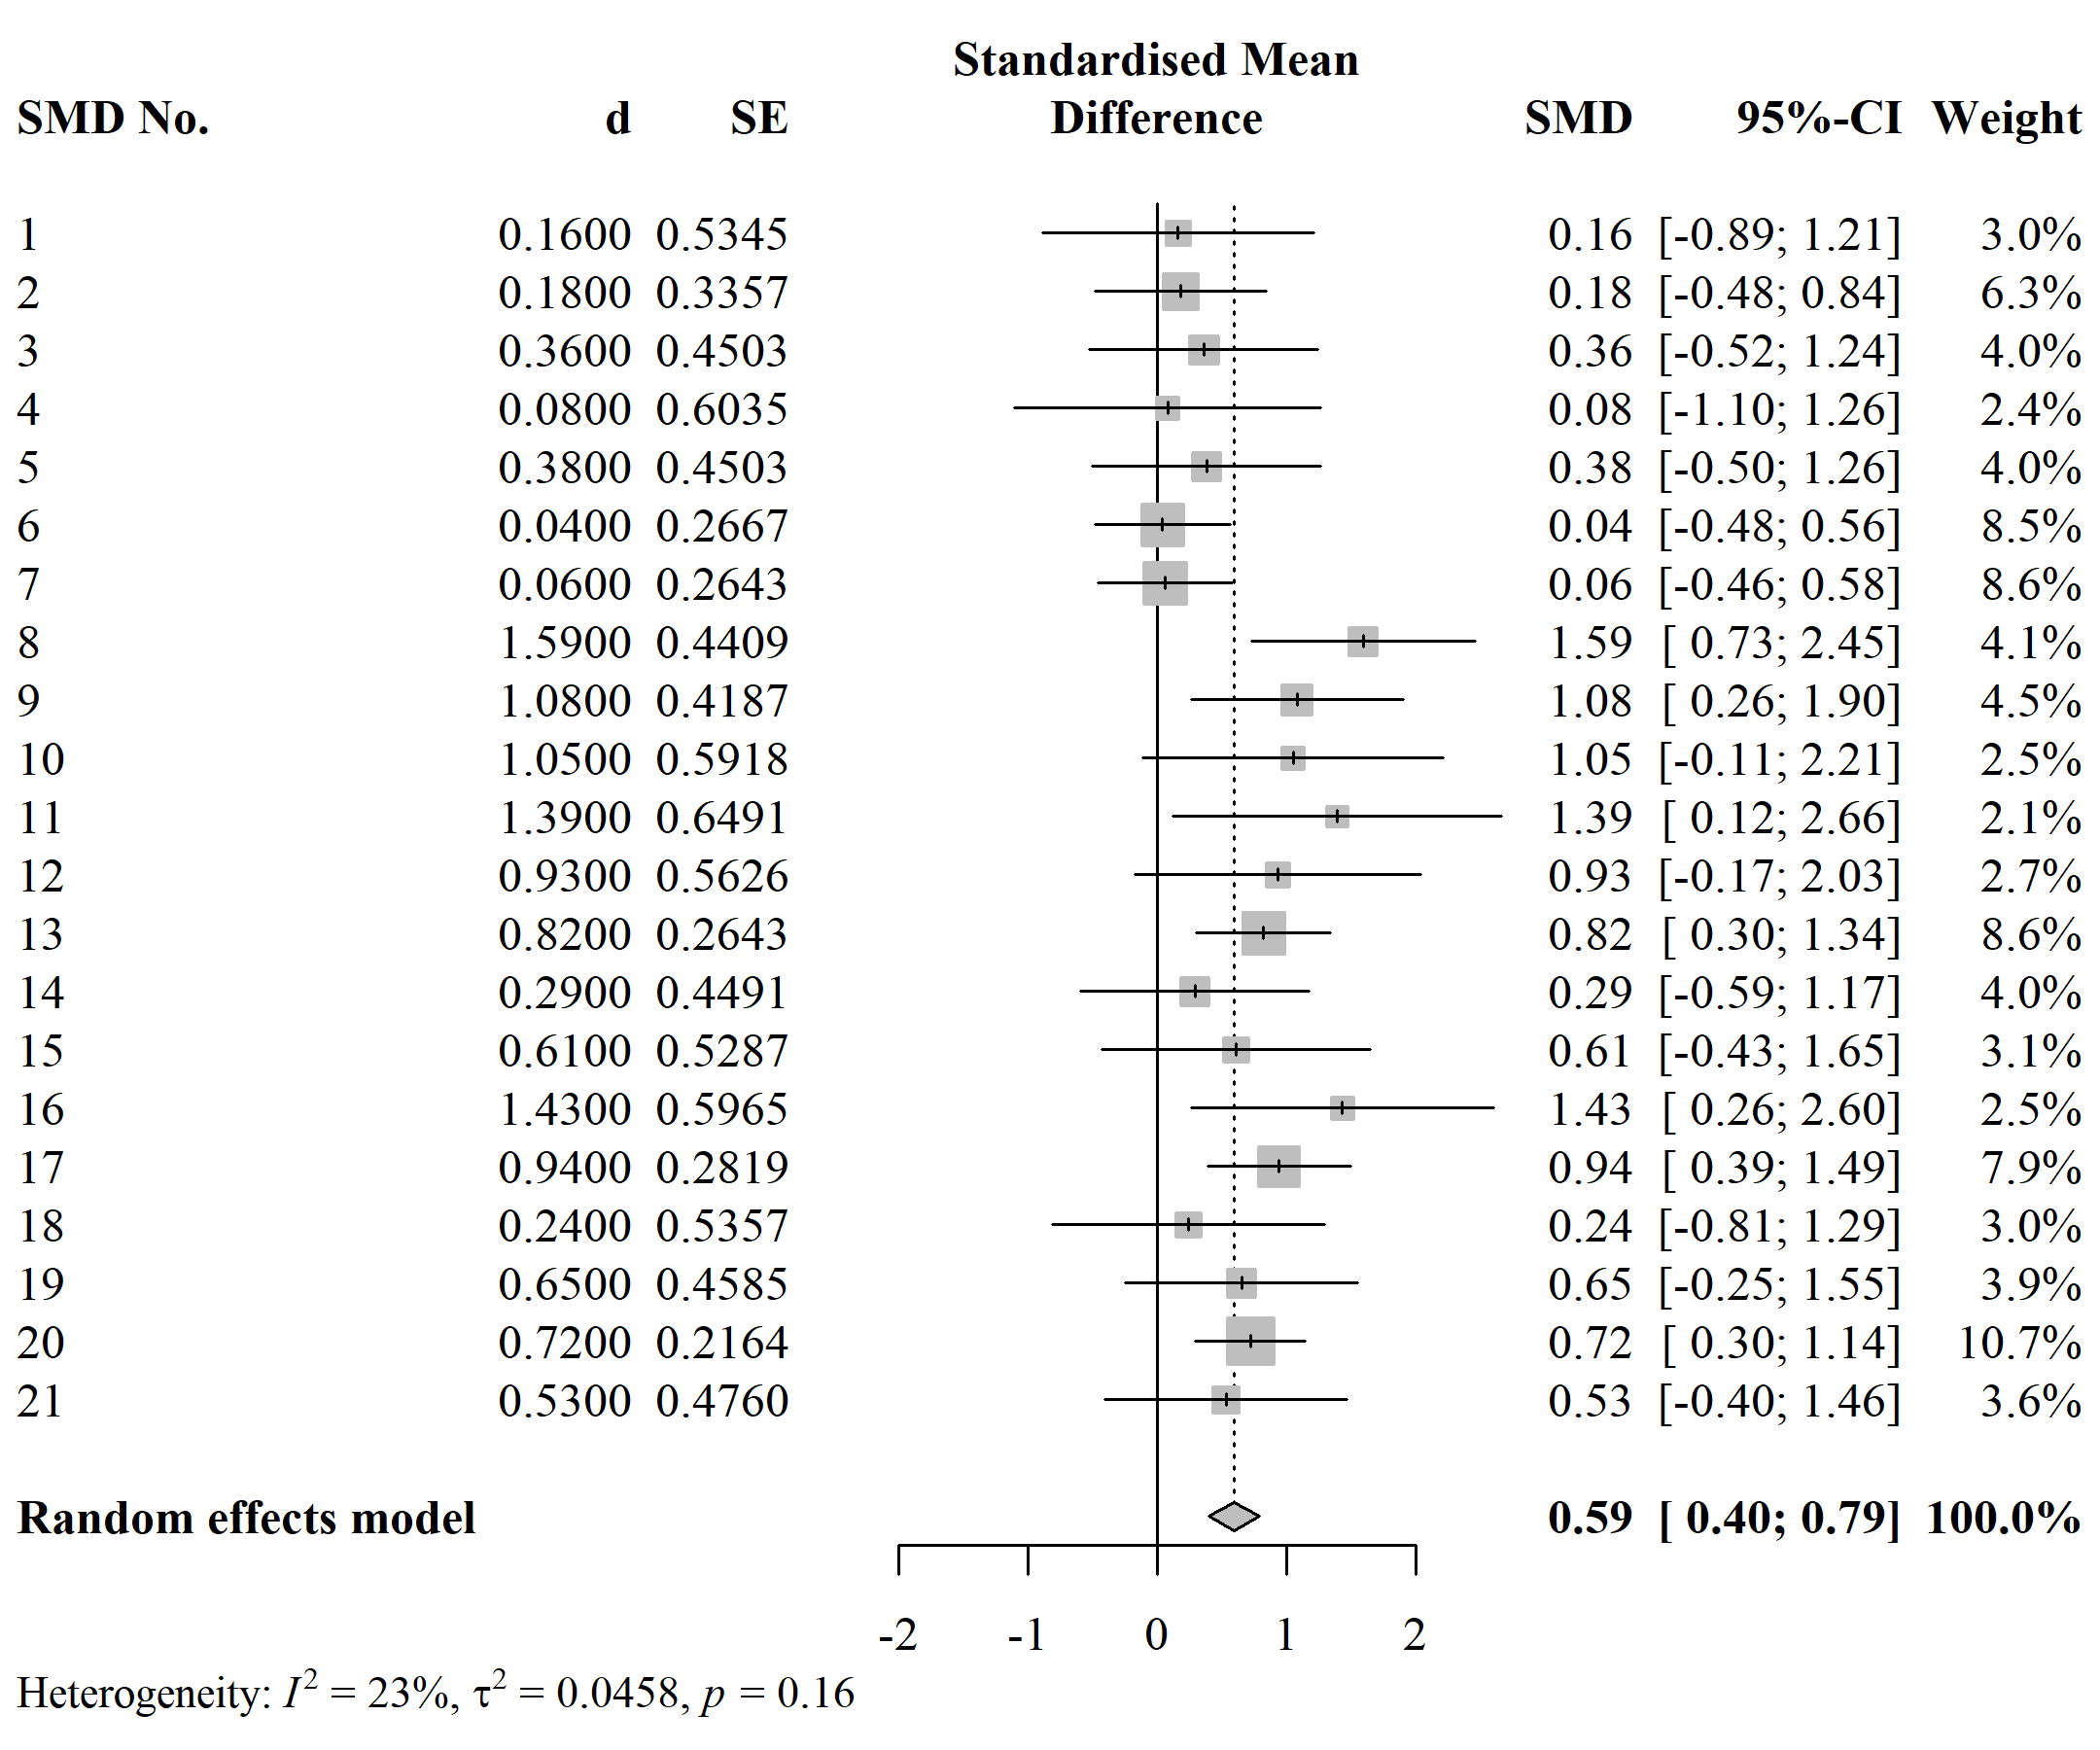
\includegraphics[width=0.5\linewidth]{figures/fig3_mam3} }

}

\caption{Forest plots of the three meta-analytic models, meta-analysis 1.}\label{fig:fig3}
\end{figure}

\hypertarget{meta-analysis-2}{%
\subsubsection{Meta-analysis 2}\label{meta-analysis-2}}

The following reproducibility-relevant information/data were reported:

\begin{itemize}
\tightlist
\item
  Standardised ES measure is SMD
\item
  Group sample sizes (\(n\)s) for each primary SMD calculated. In case of crossover studies, they reported the total sample size (\(N\)) for both the control and treatment groups.
\item
  All primary SMDs calculated
\item
  CI lower and upper limits for each SMD
\item
  The outcome measure for each SMD
\item
  SMDs were based on comparisons between cathodal tDCS group and sham group at post
\item
  random-effects model
\item
  The pooled SMD
\item
  Software used was Comprehensive Meta-Analysis
\end{itemize}

The following information was missing:

\begin{itemize}
\tightlist
\item
  Type of SMD used
\item
  Whether a different method of standardisation was used for the crossover studies
\item
  Sampling variances of the SMDs (depicted in the funnel plot)
\item
  Whether sampling variances were calculated differently for the SMDs corresponding to crossover trials
\item
  Which type of values were used to compute each SMD
\item
  Which exact values were used and where they were found
\item
  Rationale for choosing outcomes
\item
  Enough details about the outcome used so as to leave no room for ambivalence
\item
  Which between-study heterogeneity estimator was used
\end{itemize}

Table 8 summarises the reproducibility status and classification of each primary SMD. One SMD was successfully reproduced following the procedure as described in the meta-analysis or the seemingly standard procedure. Three further SMDs were approximated. Following a deviating procedure, two more SMDs were reproducible and one approximated.

\singlespacing
\begingroup\fontsize{10}{12}\selectfont

\begin{longtable}[t]{>{\raggedright\arraybackslash}p{3em}>{\raggedright\arraybackslash}p{5em}>{\raggedright\arraybackslash}p{5em}>{\raggedright\arraybackslash}p{12em}>{\raggedright\arraybackslash}p{16em}}
\caption{\label{tab:table9}Reproducibility of primary SMDs, Meta-analysis 2}\\
\toprule
SMD no. & Reported SMD & Reproduced SMD & Reproducibility classification & Reason for irreproducibility\\
\midrule
\endfirsthead
\caption[]{\label{tab:table9}Reproducibility of primary SMDs, Meta-analysis 2 \textit{(continued)}}\\
\toprule
SMD no. & Reported SMD & Reproduced SMD & Reproducibility classification & Reason for irreproducibility\\
\midrule
\endhead
\midrule
\multicolumn{5}{r@{}}{}\
\endfoot
\bottomrule
\endlastfoot
1 & 0.96 & NA & Brute-force
irreproducible & Not inferable.\\
2 & 2.46 & -0.53 & Faithfully irreproducible & Not inferable.\\
3 & 0.68 & NA & Brute-force reproducible & Brute-force reproducible but outcome used does not correspond to description.\\
4 & 1.56 & 2.59 & Faithfully irreproducible & Not inferable.\\
5 & 1.25 & 0.38 & Faithfully irreproducible & Not inferable.\\
6 & 0.28 & 0.26 & Faithfully reproducible & Not applicable.\\
7 & 0.06 & 0.17 & Faithfully irreproducible & Not inferable.\\
8 & -0.14 & NA & Brute-force reproducible & Successfully reproduced using a p-value derived from a Kruskal-Wallis test of differences between the three groups anodal, cathodal, and sham.\\
9 & -0.11 & -0.02 & Faithfully irreproducible, Brute-force reproducible & Successfully reproduced using a p-value derived from a Kruskal-Wallis test of differences between the three groups anodal, cathodal, and sham. Means and SDs were reported in the primary study for the outcome used.\\
10 & 0.94 & 0.98 & Faithfully irreproducible & Not inferable.\\
11 & 1.77 & 1.73 & Faithfully irreproducible & Not inferable.\\
12 & 0.37 & 0.26 & Faithfully irreproducible & Not inferable.\\
13 & 0.34 & -0.03 & Faithfully irreproducible & Not inferable.\\
14 & 2.10 & 0.31 & Faithfully irreproducible & Not inferable.\\
15 & 1.18 & 0.12 & Faithfully irreproducible & Not inferable.\\
16 & 0.08 & -0.08 & Faithfully irreproducible & Wrong sign.\\
17 & 0.75 & 0.75 & Faithfully reproducible & Not applicable.\\
18 & 0.61 & 0.62 & Faithfully reproducible & Not applicable.\\
19 & -0.87 & -0.95 & Faithfully reproducible & Not applicable.\\
20 & 0.90 & 1.41 & Faithfully irreproducible & Not inferable.\\*
\end{longtable}

1 \& Faithfully irreproducible \& Not inferable.\textbackslash*
\textbackslash end\{longtable\}
\endgroup{}
\doublespacing

All meta-analytic estimates were successfully reproduced in MAM 3, whose output was again treated as ``reported''. The three MAMs are depicted in Figure 4. The pooled SMDs from MAMs 1 and 2 deviate from the reported pooled SMD by 0.17 and 0.22 SDs, respectively. All three models displayed a very high degree of heterogeneity.
\newpage

\begin{figure}[H]

{\centering \subfloat[MAM 1, based on faithfully reproduced SMDs.\label{fig:fig4-1}]{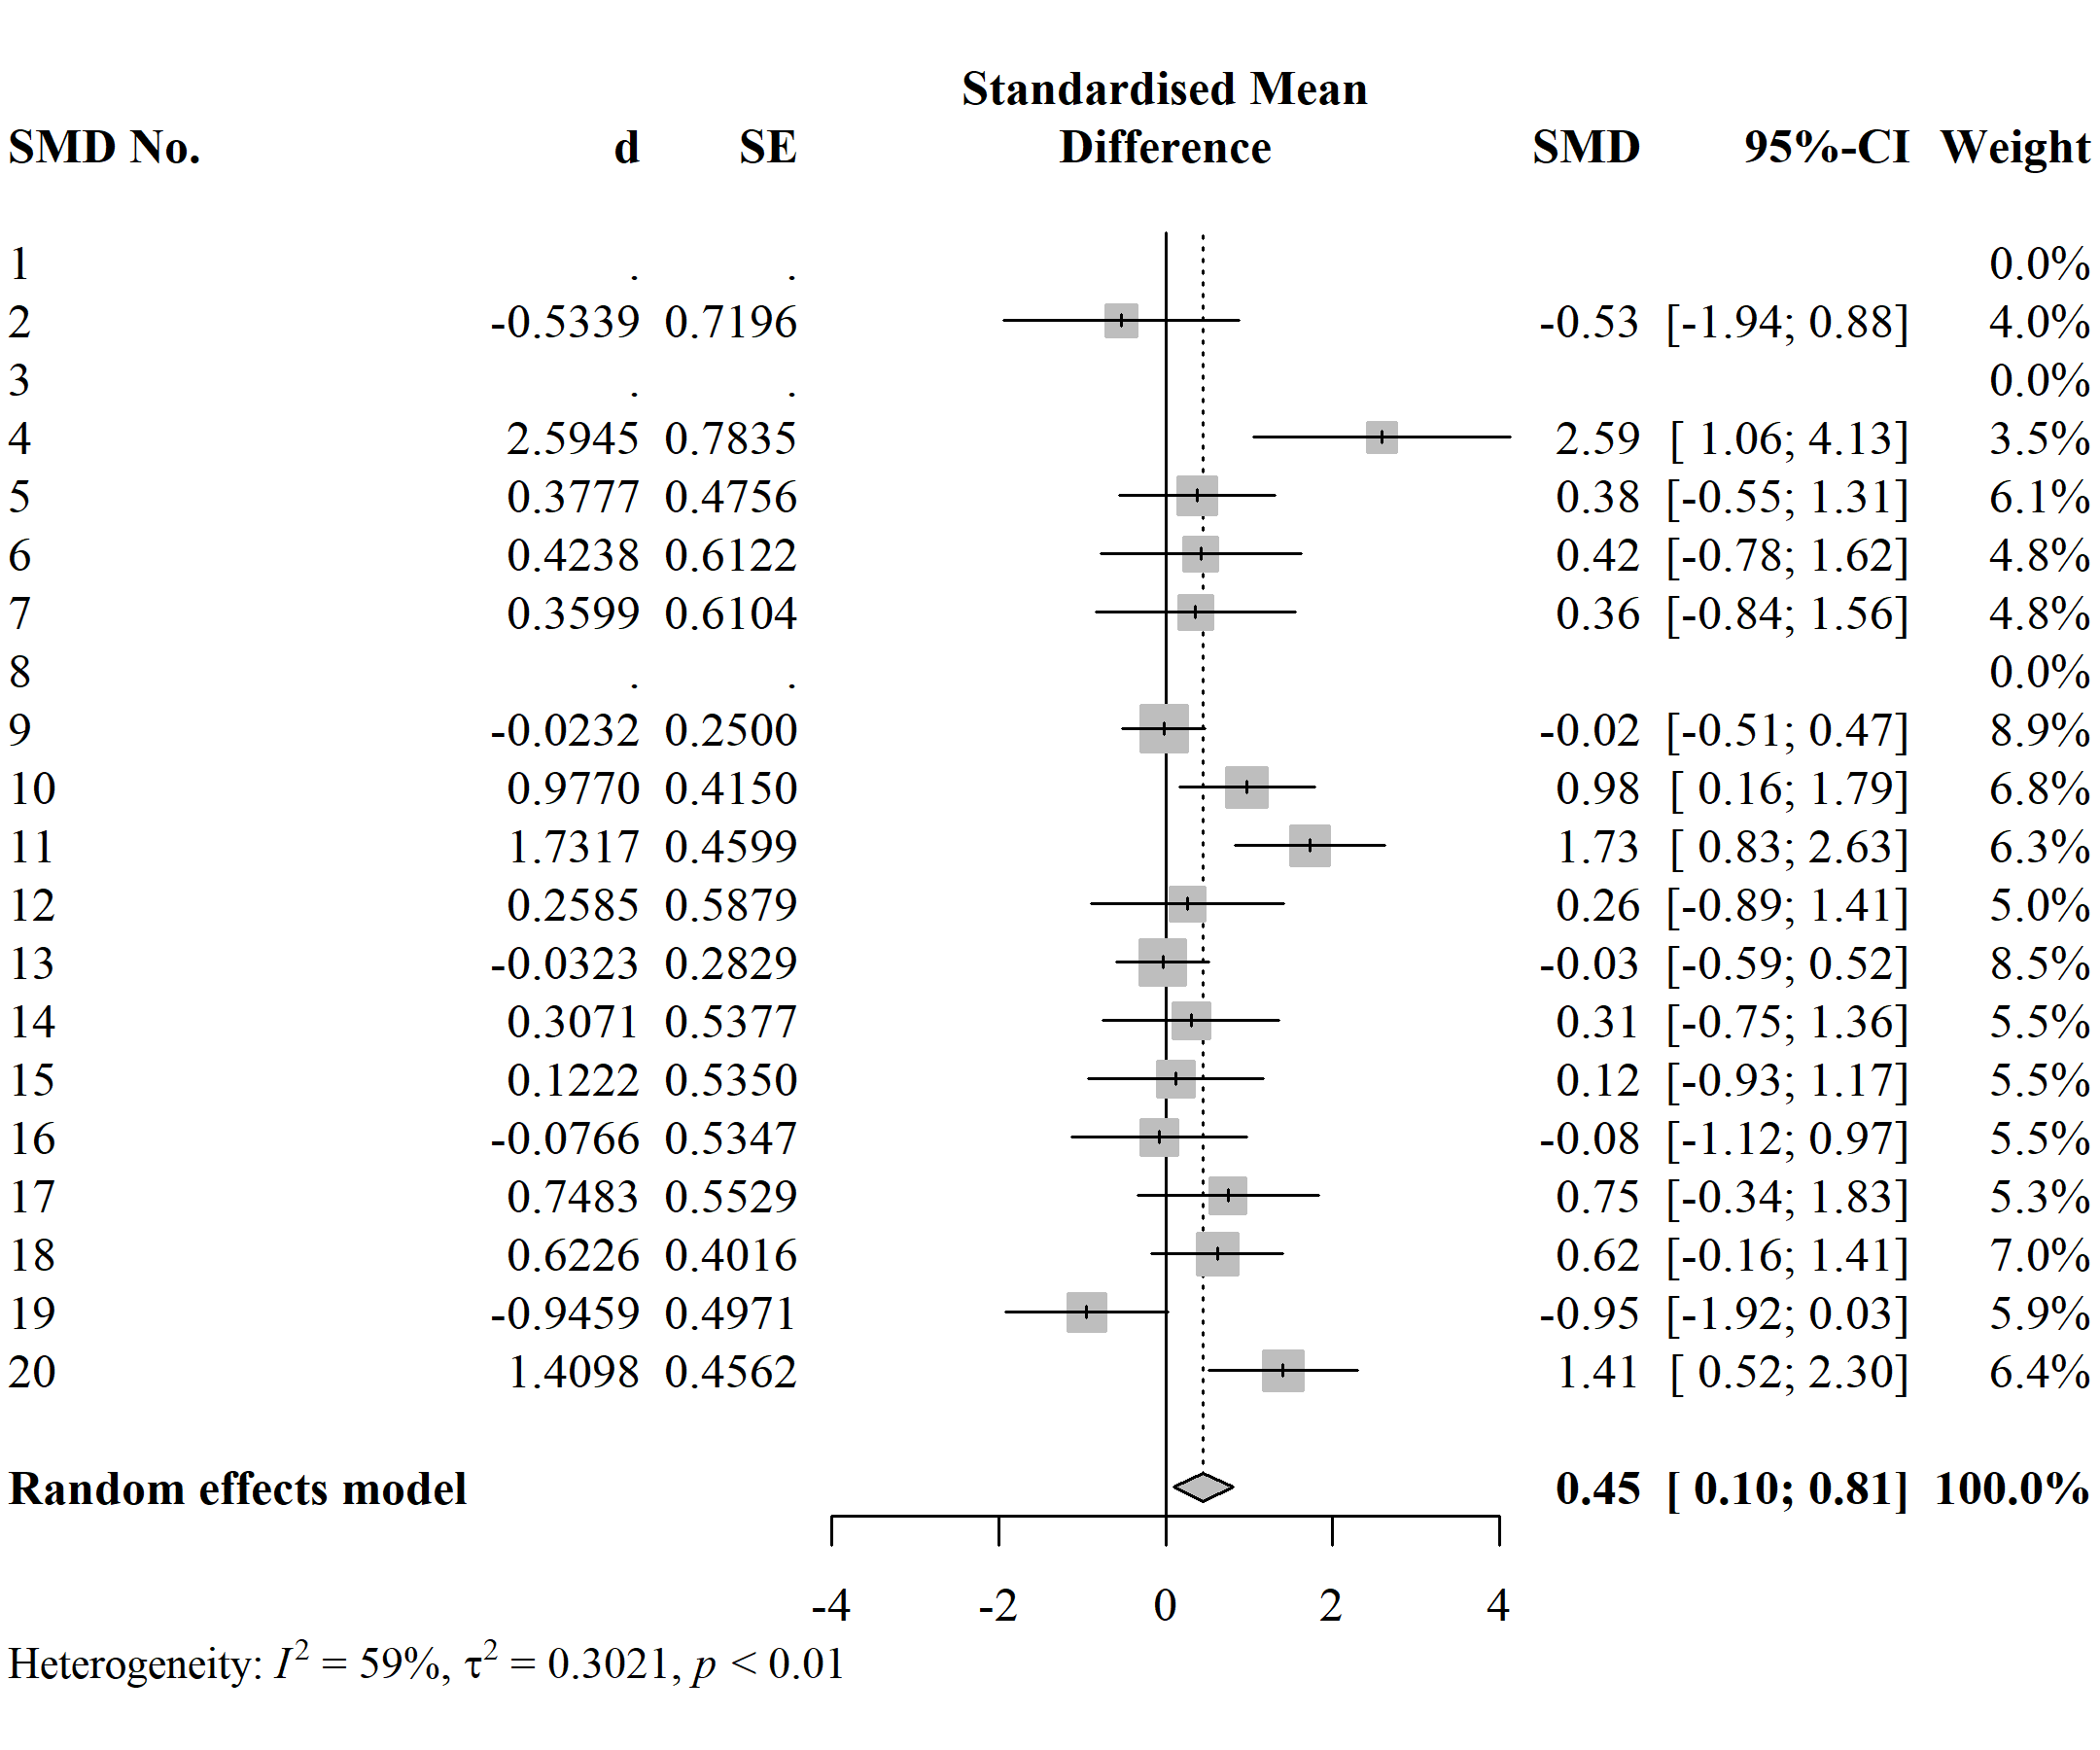
\includegraphics[width=0.5\linewidth]{figures/fig4_mam1} }\subfloat[MAM 2, based on faithfully and brute-force reproduced SMDs.\label{fig:fig4-2}]{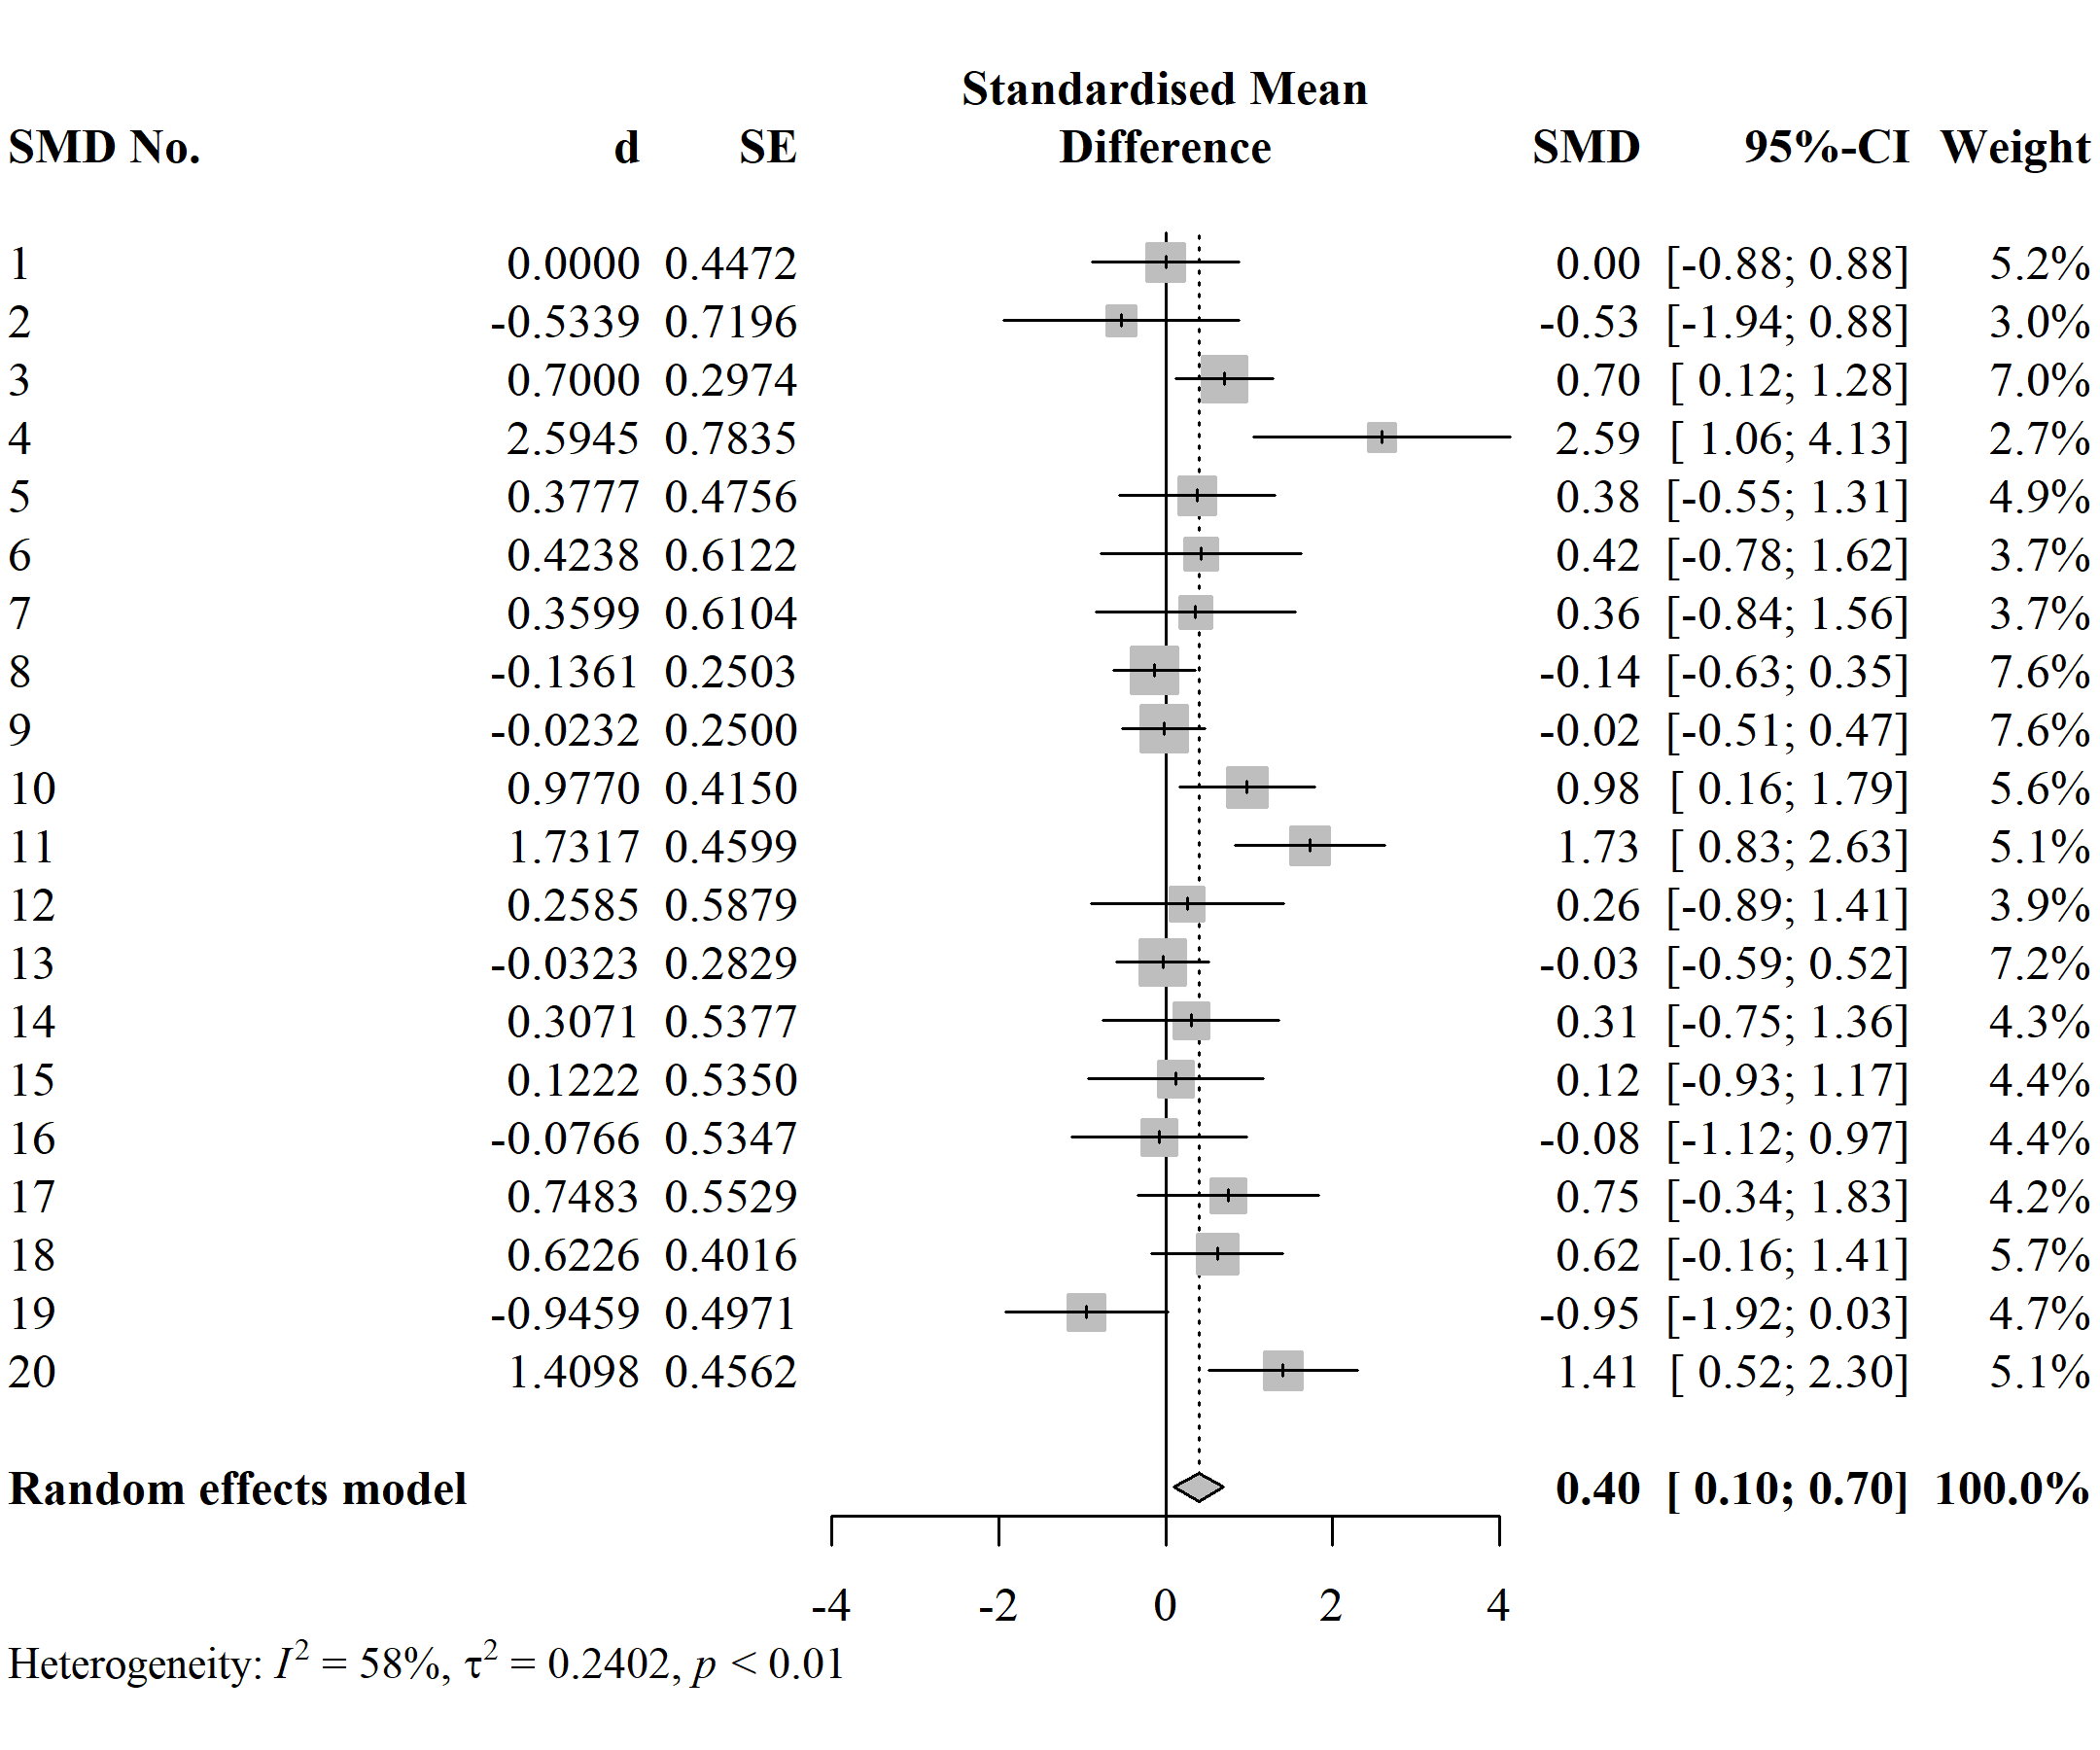
\includegraphics[width=0.5\linewidth]{figures/fig4_mam2} }\newline\subfloat[MAM 3, based on reported SMDs.\label{fig:fig4-3}]{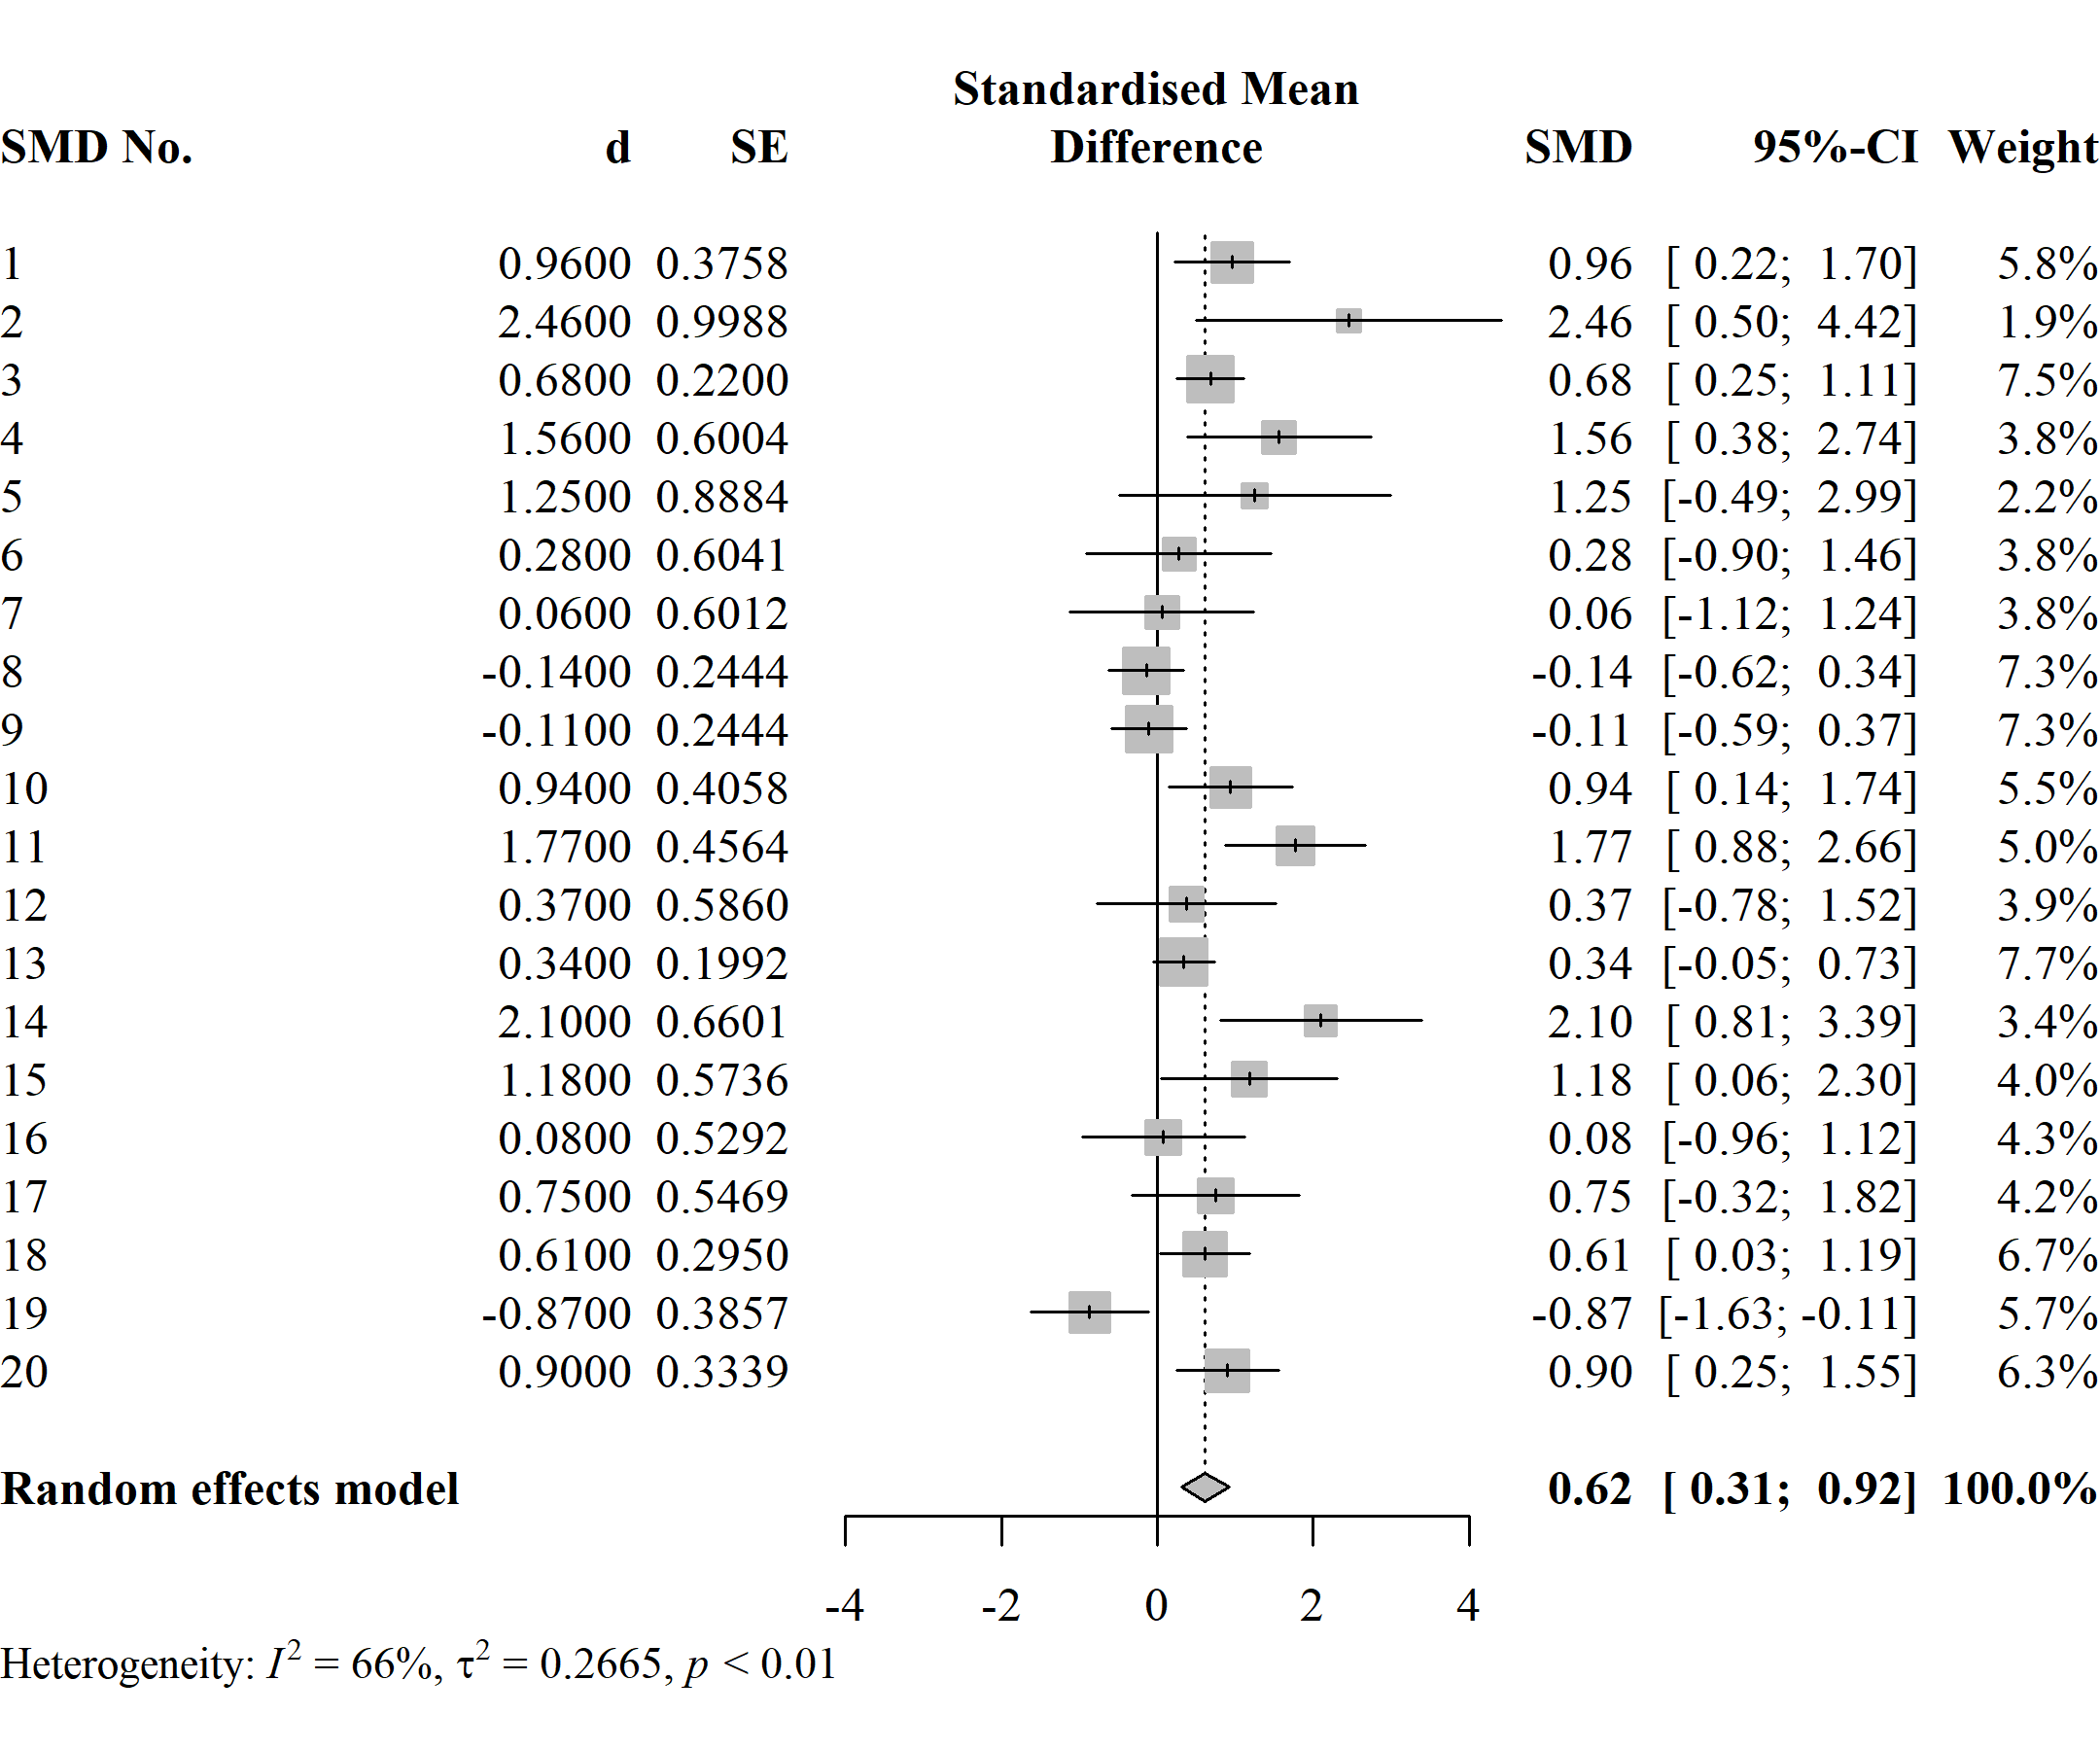
\includegraphics[width=0.5\linewidth]{figures/fig4_mam3} }

}

\caption{Forest plots of the three meta-analytic models, meta-analysis 2.}\label{fig:fig4}
\end{figure}

\hypertarget{meta-analysis-3}{%
\subsubsection{Meta-analysis 3}\label{meta-analysis-3}}

The following reproducibility-relevant information/data were reported:

\begin{itemize}
\tightlist
\item
  Standardised ES measure is Hedges' \(g\)
\item
  Group sample sizes (\(n\)s) for each primary SMD calculated. In case of crossover studies, they reported the total sample size (\(N\)) for both the control and treatment groups.
\item
  All primary SMDs calculated
\item
  CI lower and upper limits for each SMD
\item
  The outcome measure used for each primary study was what the primary study defined as the primary outcome
\item
  SMDs were based on comparisons between tDCS group and sham group at post
\item
  The task learned by participants (which sometimes aided in finding the outcome used by the meta-analysts)
\item
  The pooled SMD
\item
  Software used was Comprehensive Meta-Analysis
\end{itemize}

The following information was missing:

\begin{itemize}
\tightlist
\item
  Whether a different method of standardisation was used for the crossover study
\item
  Sampling variances of the SMDs
\item
  Whether sampling variances were calculated differently for the SMD corresponding to the crossover trial
\item
  Which type of values were used to compute each SMD
\item
  Which exact values were used and where they were found
\item
  Enough details about the outcome used so as to leave no room for ambivalence
\item
  Which between-study heterogeneity estimator was used
\end{itemize}

Table 9 summarises the reproducibility status and classification of each primary SMD. One SMD was approximated following the procedure as described in the meta-analysis or the seemingly standard procedure. Following a deviating procedure, all 5 remaining SMDs could be reproduced or approximated.

\newpage
\singlespacing
\begingroup\fontsize{10}{12}\selectfont

\begin{longtable}[t]{>{\raggedright\arraybackslash}p{3em}>{\raggedright\arraybackslash}p{5em}>{\raggedright\arraybackslash}p{5em}>{\raggedright\arraybackslash}p{12em}>{\raggedright\arraybackslash}p{16em}}
\caption{\label{tab:table10}Reproducibility of primary SMDs, Meta-analysis 3}\\
\toprule
SMD no. & Reported SMD & Reproduced SMD & Reproducibility classification & Reason for irreproducibility\\
\midrule
1 & 0.84 & NA & Brute-force reproducible & Successfully reproduced using a p-value (reported in the primary study as a range "<0.01") derived from a difference in medians test.\\
2 & 0.25 & 0.27 & Faithfully irreproducible, Brute-force reproducible & Successfully reproduced using the values for one of the two outcomes indicated to have been used and doubling the tDCS group sample size.\\
3 & 0.98 & NA & Brute-force reproducible & Sucessfully reproduced using a p-value (reported as a range "<0.01") derived from a medians test in combination with the total sample size in place of both treatment and control group sample sizes. Notably, this was not a journal article, but a conference abstract.\\
4 & 1.19 & NA & Brute-force reproducible & Outcome used does not correspond to description.\\
5 & 0.59 & 0.56 & Faithfully reproducible & Not applicable.\\
6 & 0.58 & NA & Brute-force reproducible & Successfully reproduced using a p-value based on difference between tDCS and sham groups in change from baseline\\
\bottomrule
\end{longtable}
\endgroup{}
\vspace{-9mm}
\begin{tablenotes}[para,flushleft]
      \small
      \item \textit{Note.} The reported SMDs were rounded to the second decimal (3 decimals were reported).
    \end{tablenotes}
\doublespacing

Using the SMDs and the sample sizes reported in the meta-analysis along with the sampling variances calculated based on the reported CIs, all meta-analytic estimates were successfully reproduced. The output of this MAM (3) was thus again treated as the reported variety and used for comparison. The three MAMs are depicted in Figure 4. The pooled SMD from MAM 1 deviates from the reported pooled SMD by 0.24 SDs, whereas MAM 2 is almost identical to the MAM 3. Very little heterogeneity was observed in all three cases.

\newpage
\begin{figure}[H]

{\centering \subfloat[MAM 1, based on faithfully reproduced SMDs.\label{fig:fig5-1}]{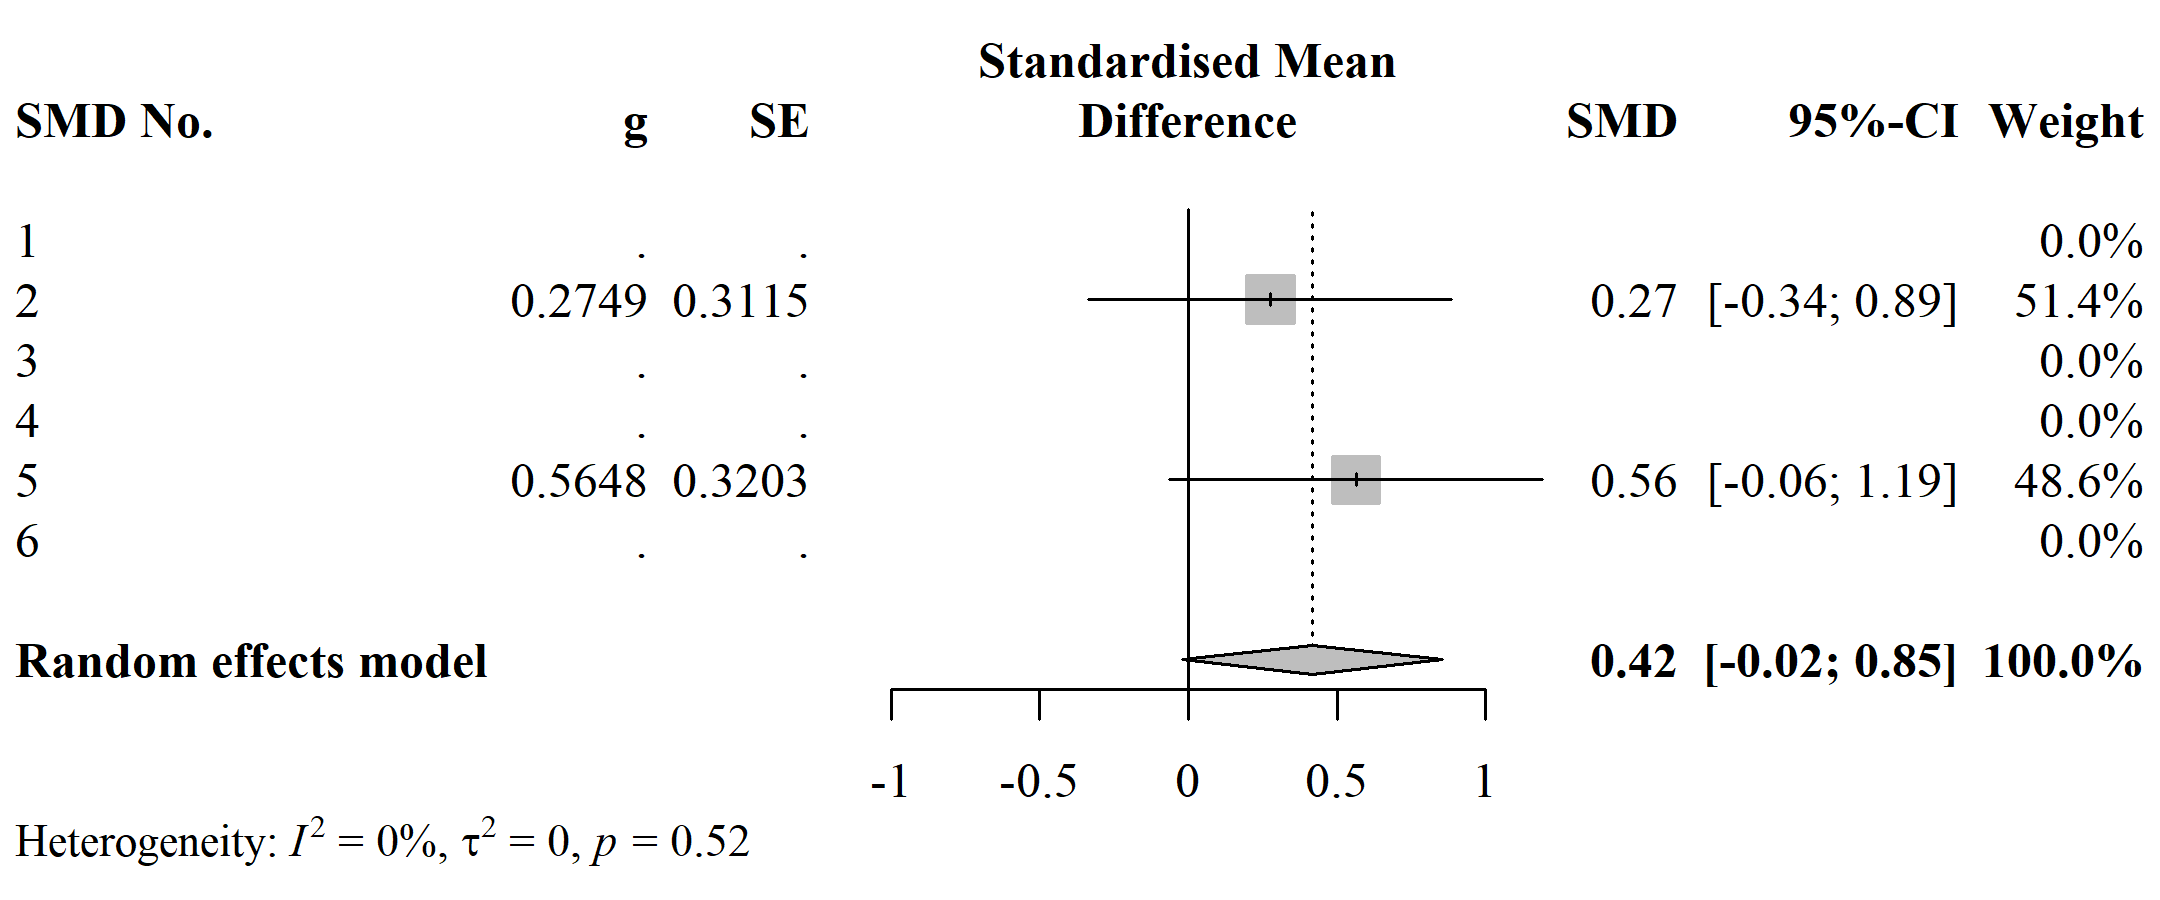
\includegraphics[width=0.5\linewidth]{figures/fig5_mam1} }\subfloat[MAM 2, based on faithfully and brute-force reproduced SMDs.\label{fig:fig5-2}]{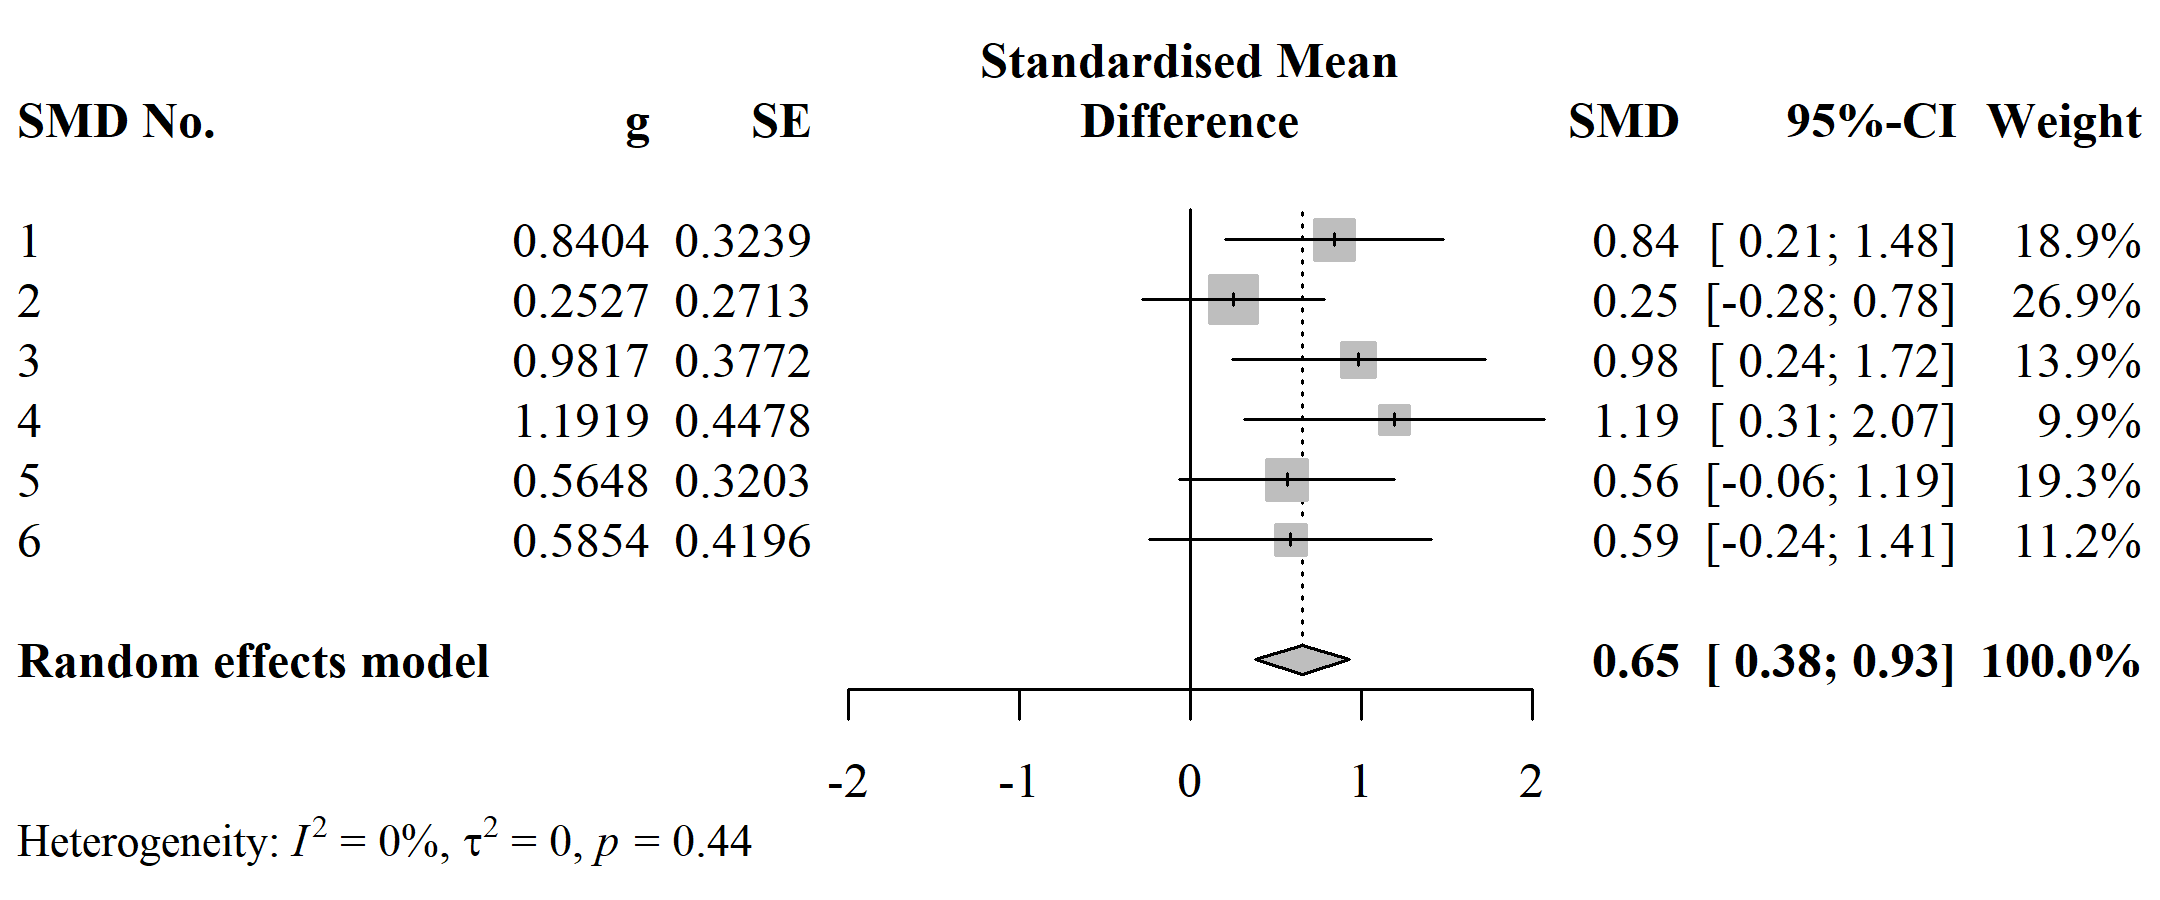
\includegraphics[width=0.5\linewidth]{figures/fig5_mam2} }\newline\subfloat[MAM 3, based on reported SMDs.\label{fig:fig5-3}]{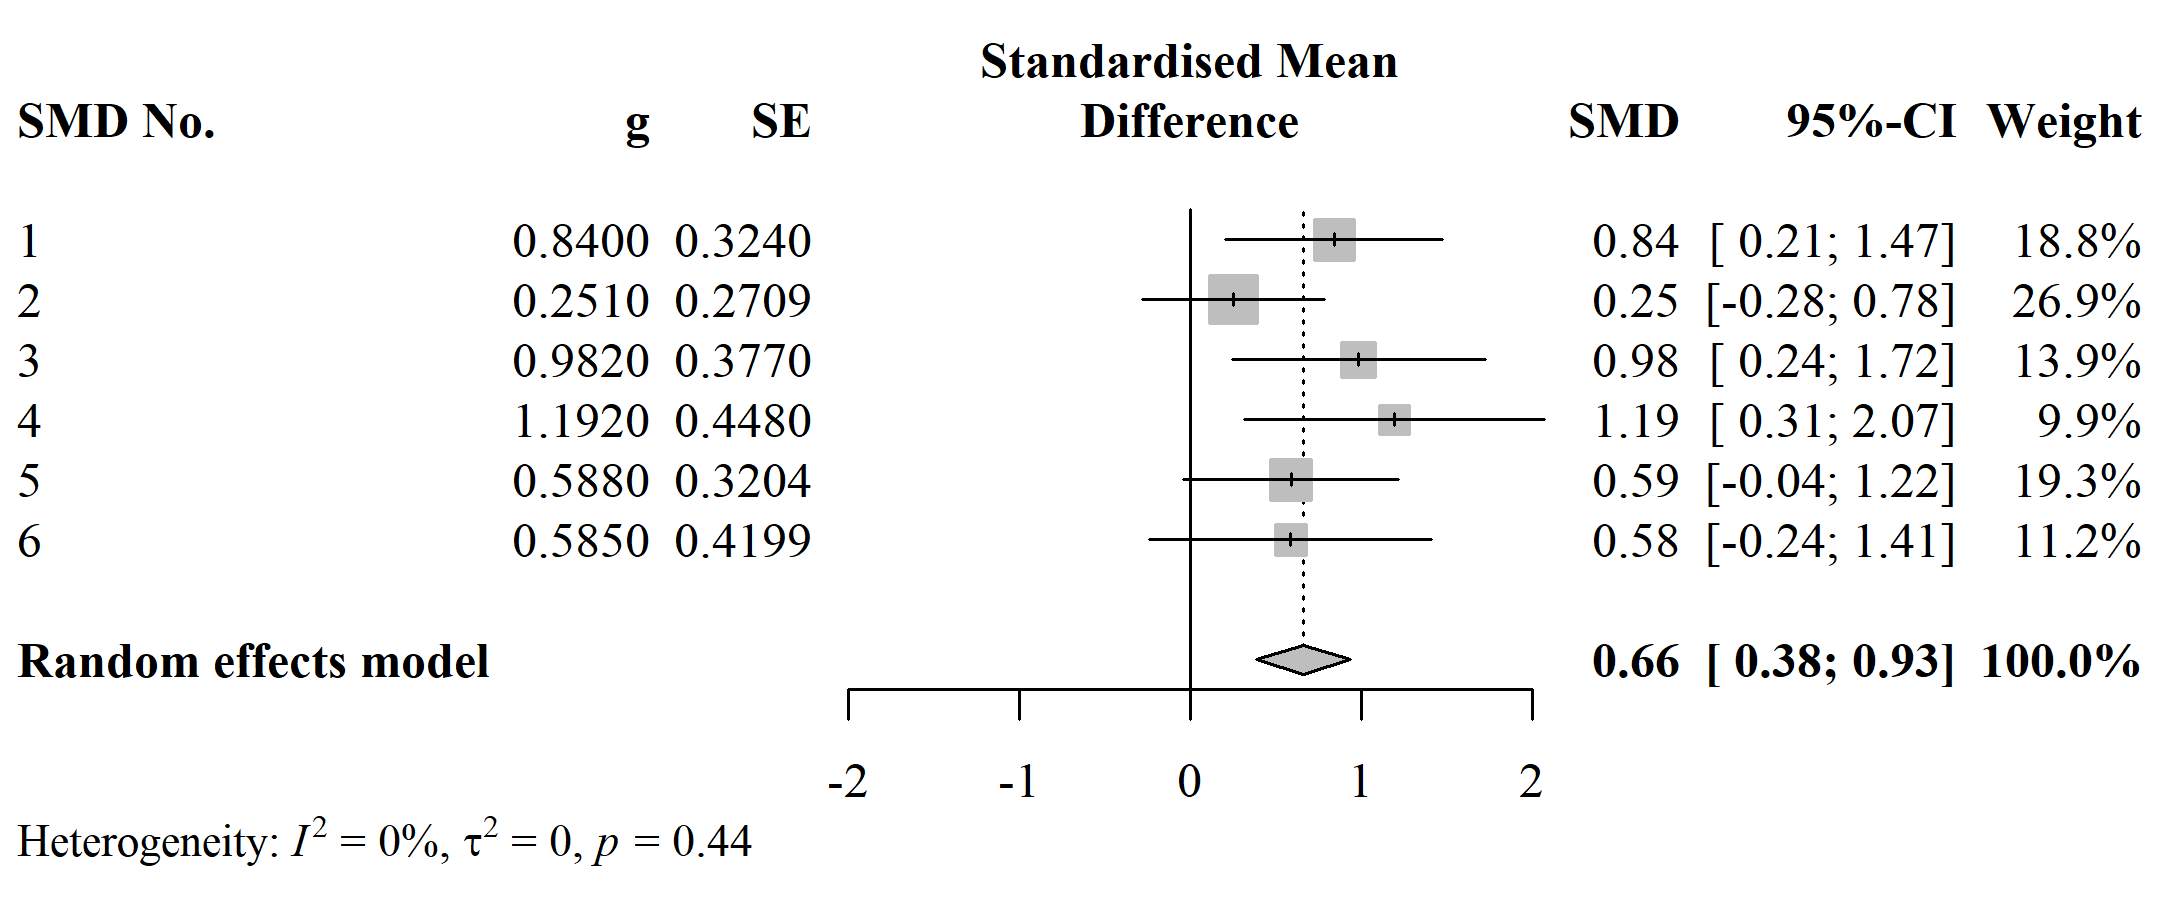
\includegraphics[width=0.5\linewidth]{figures/fig5_mam3} }

}

\caption{Forest plots of the three meta-analytic models, meta-analysis 3.}\label{fig:fig5}
\end{figure}

\hypertarget{publication-bias-control-2}{%
\subsection{Publication bias control}\label{publication-bias-control-2}}

All three meta-analyses mentioned publication bias, although only meta-analysis 3 reported having taken measures to pre-emptively mitigate its effects: the authors report having searched ClinicalTrials.gov and ProQuest (which indexes theses and dissertations), contacted the authors of the primary studies to ask for more data, and not restricted their search to articles written in English.

All three meta-analyses report having inspected a funnel plot as a means to detect publication bias. Meta-analysis 1 additionally used Fail-Safe \(N\). To correct for publication bias, meta-analysis 1 used trim-and-fill; meta-analysis 2 used trim-and-fill, Egger's test, and Begg and Maxumdar's rank correlation test (Begg \& Mazumdar, 1994); meta-analysis 3 used Egger's test. The authors of meta-analysis 1 concluded that the findings of the tests they used ``support a minor publication bias conclusion'' (Kang et al., 2016, p. 348). Similarly, the conclusion in meta-analysis 2 (Kang et al., 2018, p. 5) was ``minimal publication bias in the studies used''. No clear conclusion was provided in meta-analysis 3.

Our publication bias testing routine (along with the associated decision rule pre-defined in the data analysis plan) indicated a conclusion concurring with that of the meta-analysts in the case of the first meta-analysis and the opposite conclusions for the two other meta-analyses. For meta-analysis 1, the estimate of the true effect produced by the three-parameter selection model (0.59) was virtually identical to the original. The estimate produced by the \(p\)-curve was larger (0.70). Only the PET-PEESE intercepts (0.34 and 0.45, respectively) indicated that the random-effects model based estimates might be overestimating the true effect. For meta-analysis 2, the selection model (0.20), \(p\)-curve (0.18), and PEESE (0.21) estimates were much smaller than the original (0.62). The PET intercept (-0.12) was negative. Similar results were observed for the last meta-analysis: the estimates produced by the the \(p\)-curve and PET-PEESE were 0.40, -0.71, and 0.01, respectively. Only the selection model yielded an estimate which is close to the one based on the random-effects model (0.62).

\hypertarget{outlierinfluential-study-analysis-1}{%
\subsubsection{Outlier/influential study analysis}\label{outlierinfluential-study-analysis-1}}

Only the third meta-analysis mentioned outliers or influential studies. They ran a leave-one-out analysis and reported that the main results did not change due to removing any one of the 6 studies they included. Our leave-one-out analysis indicated the presence of influential studies in all three meta-analyses (see Figure 6).

\newpage
\begin{figure}[H]

{\centering \subfloat[Meta-analysis 1.\label{fig:fig6-1}]{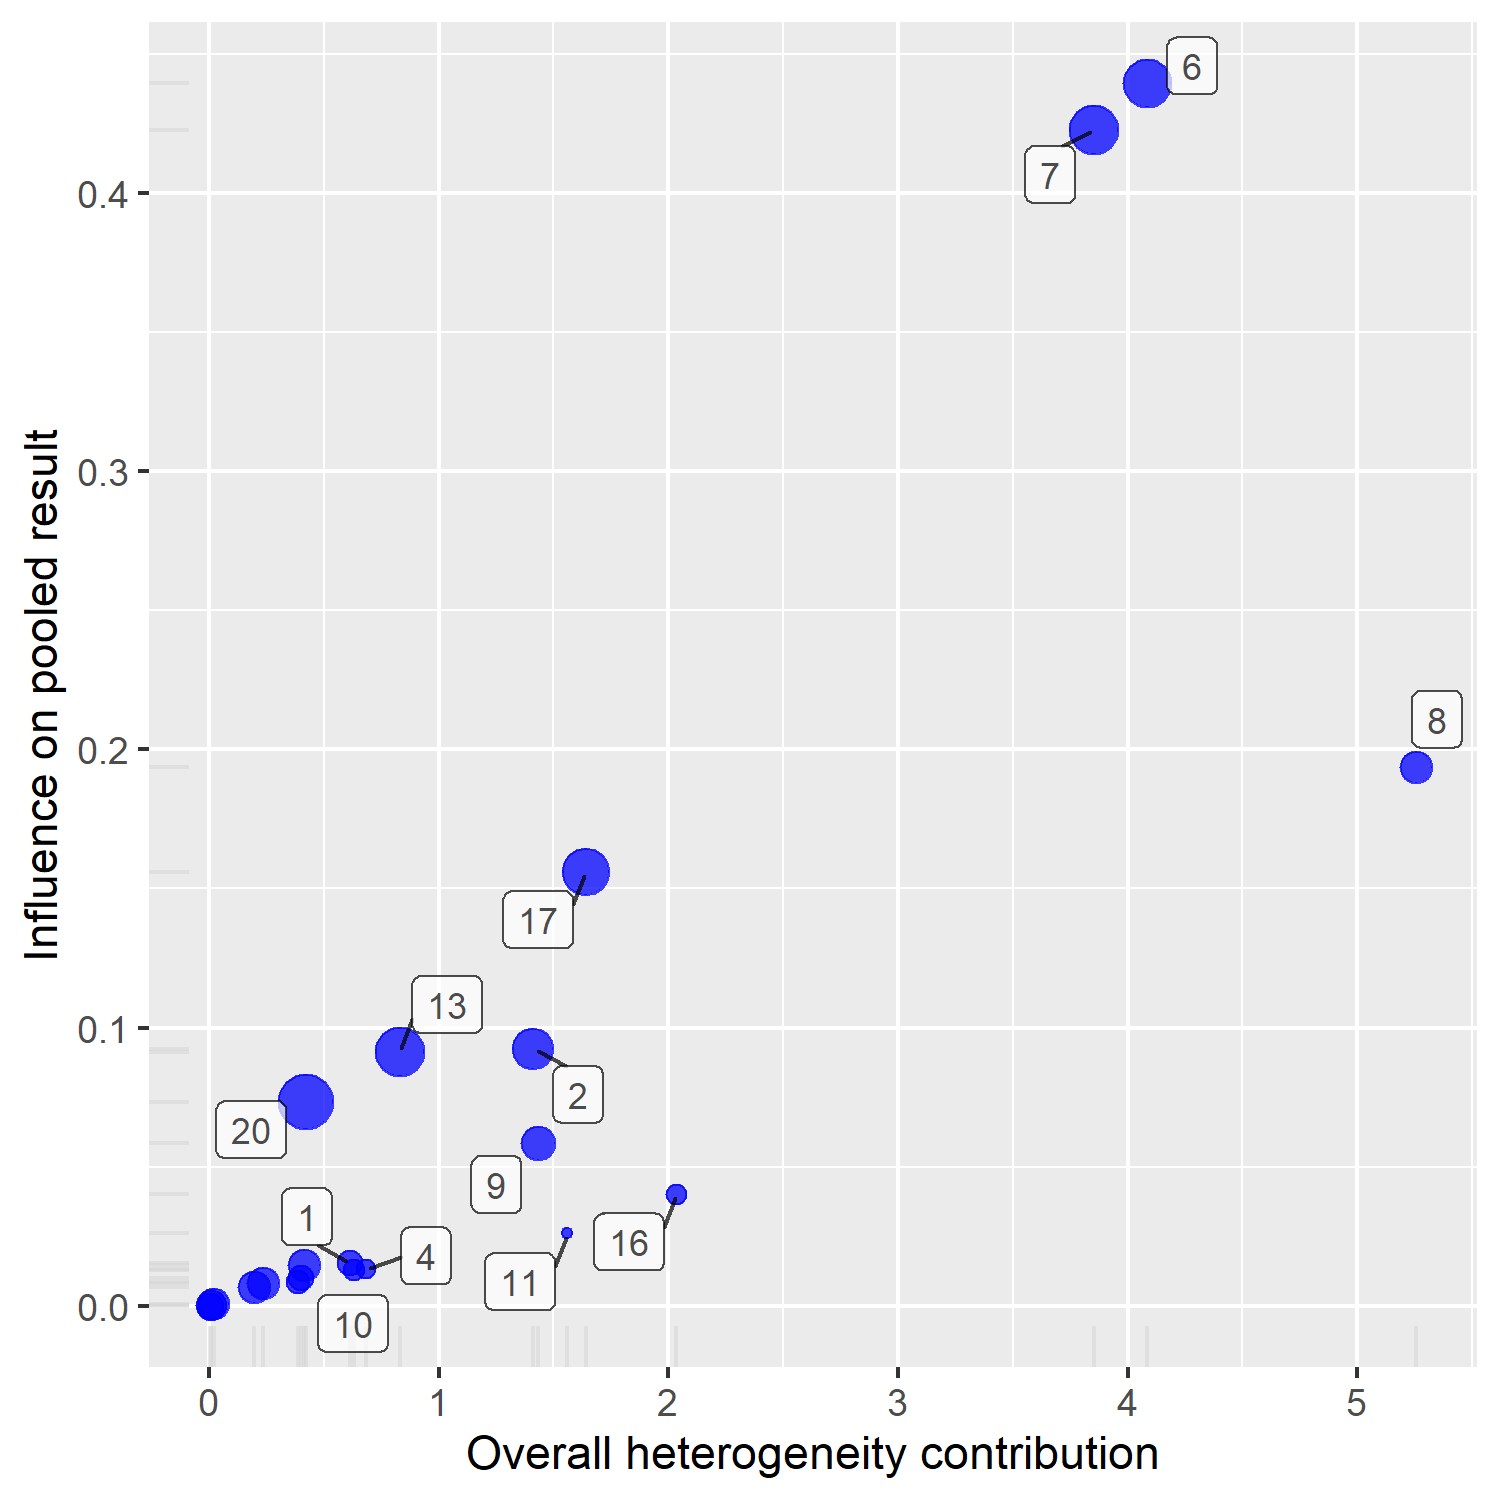
\includegraphics[width=0.5\linewidth]{figures/fig6} }\subfloat[Meta-analysis 2.\label{fig:fig6-2}]{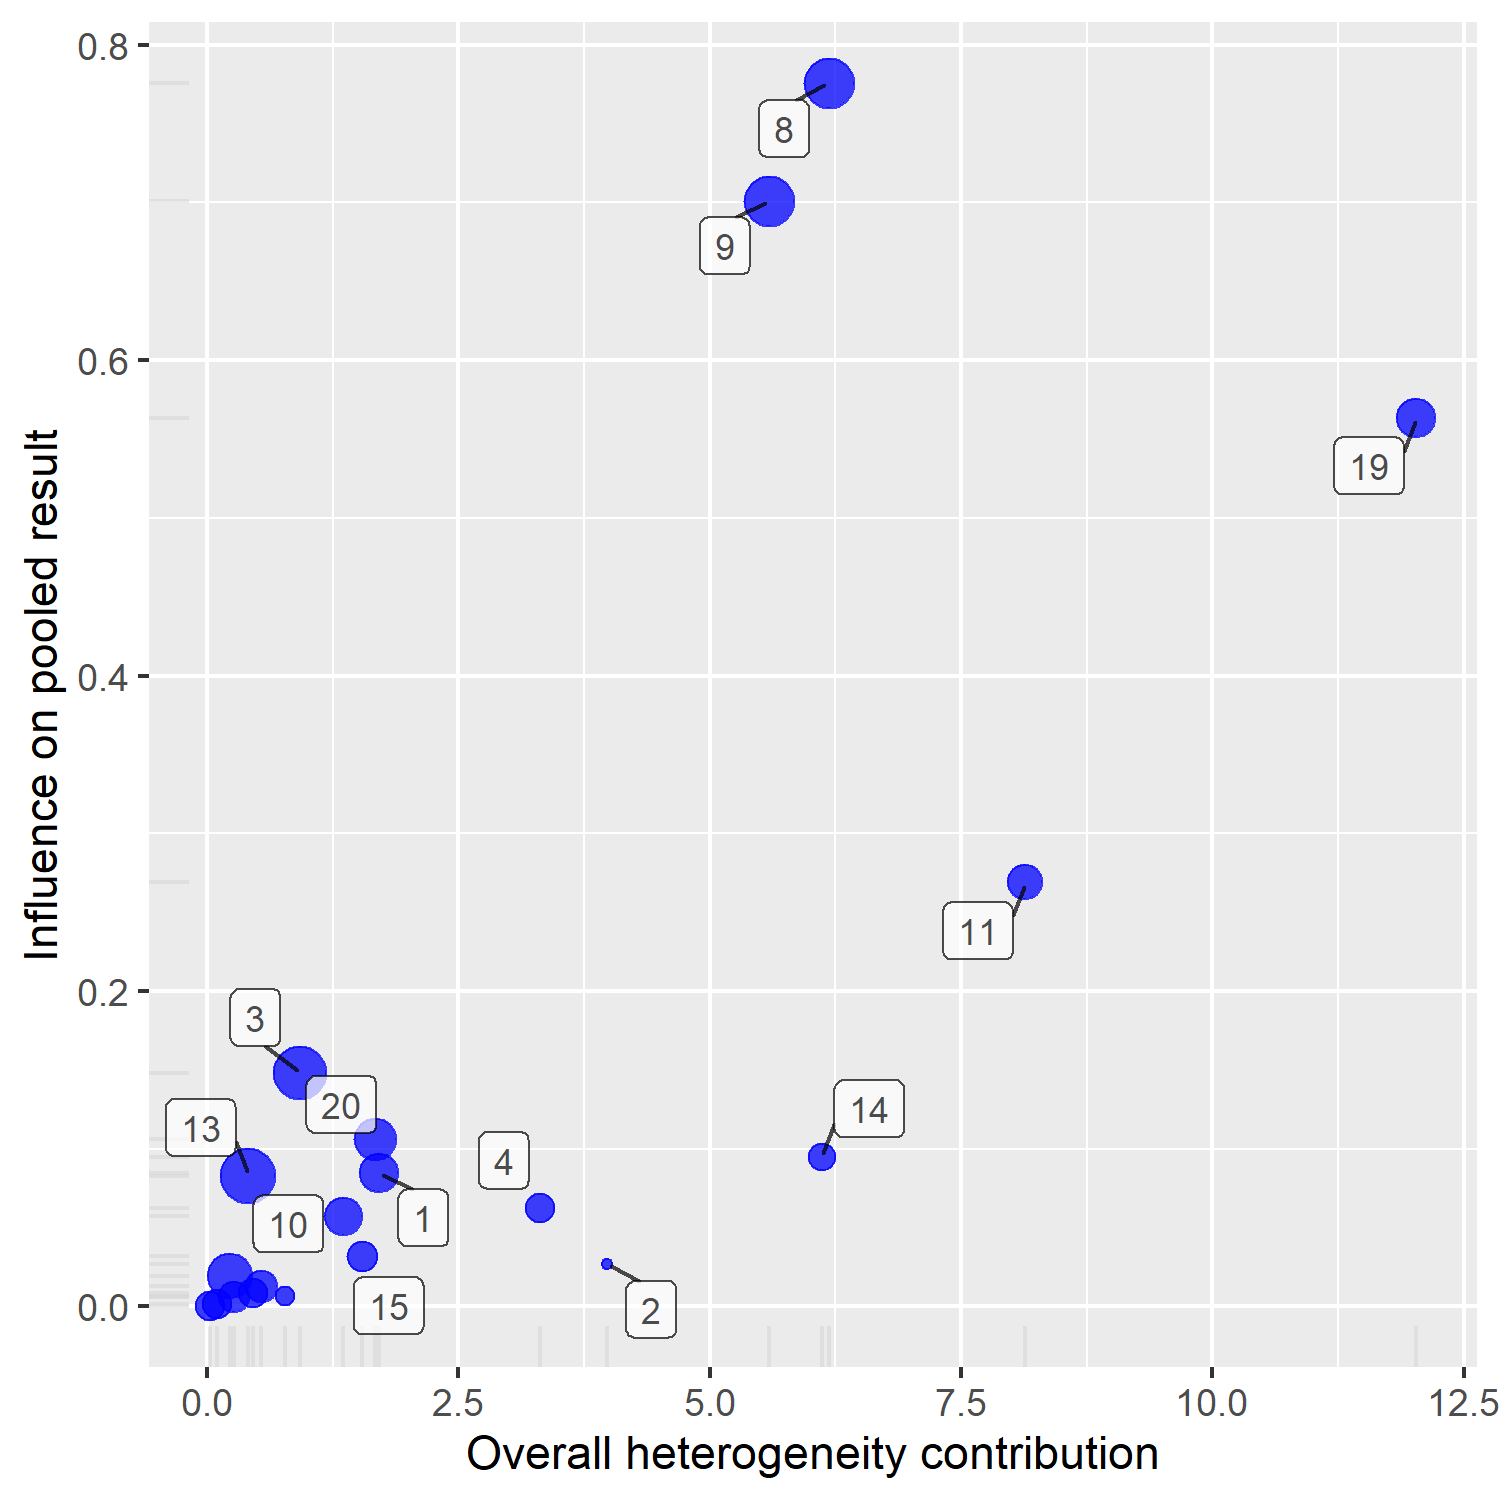
\includegraphics[width=0.5\linewidth]{figures/fig7} }\newline\subfloat[Meta-analysis 3.\label{fig:fig6-3}]{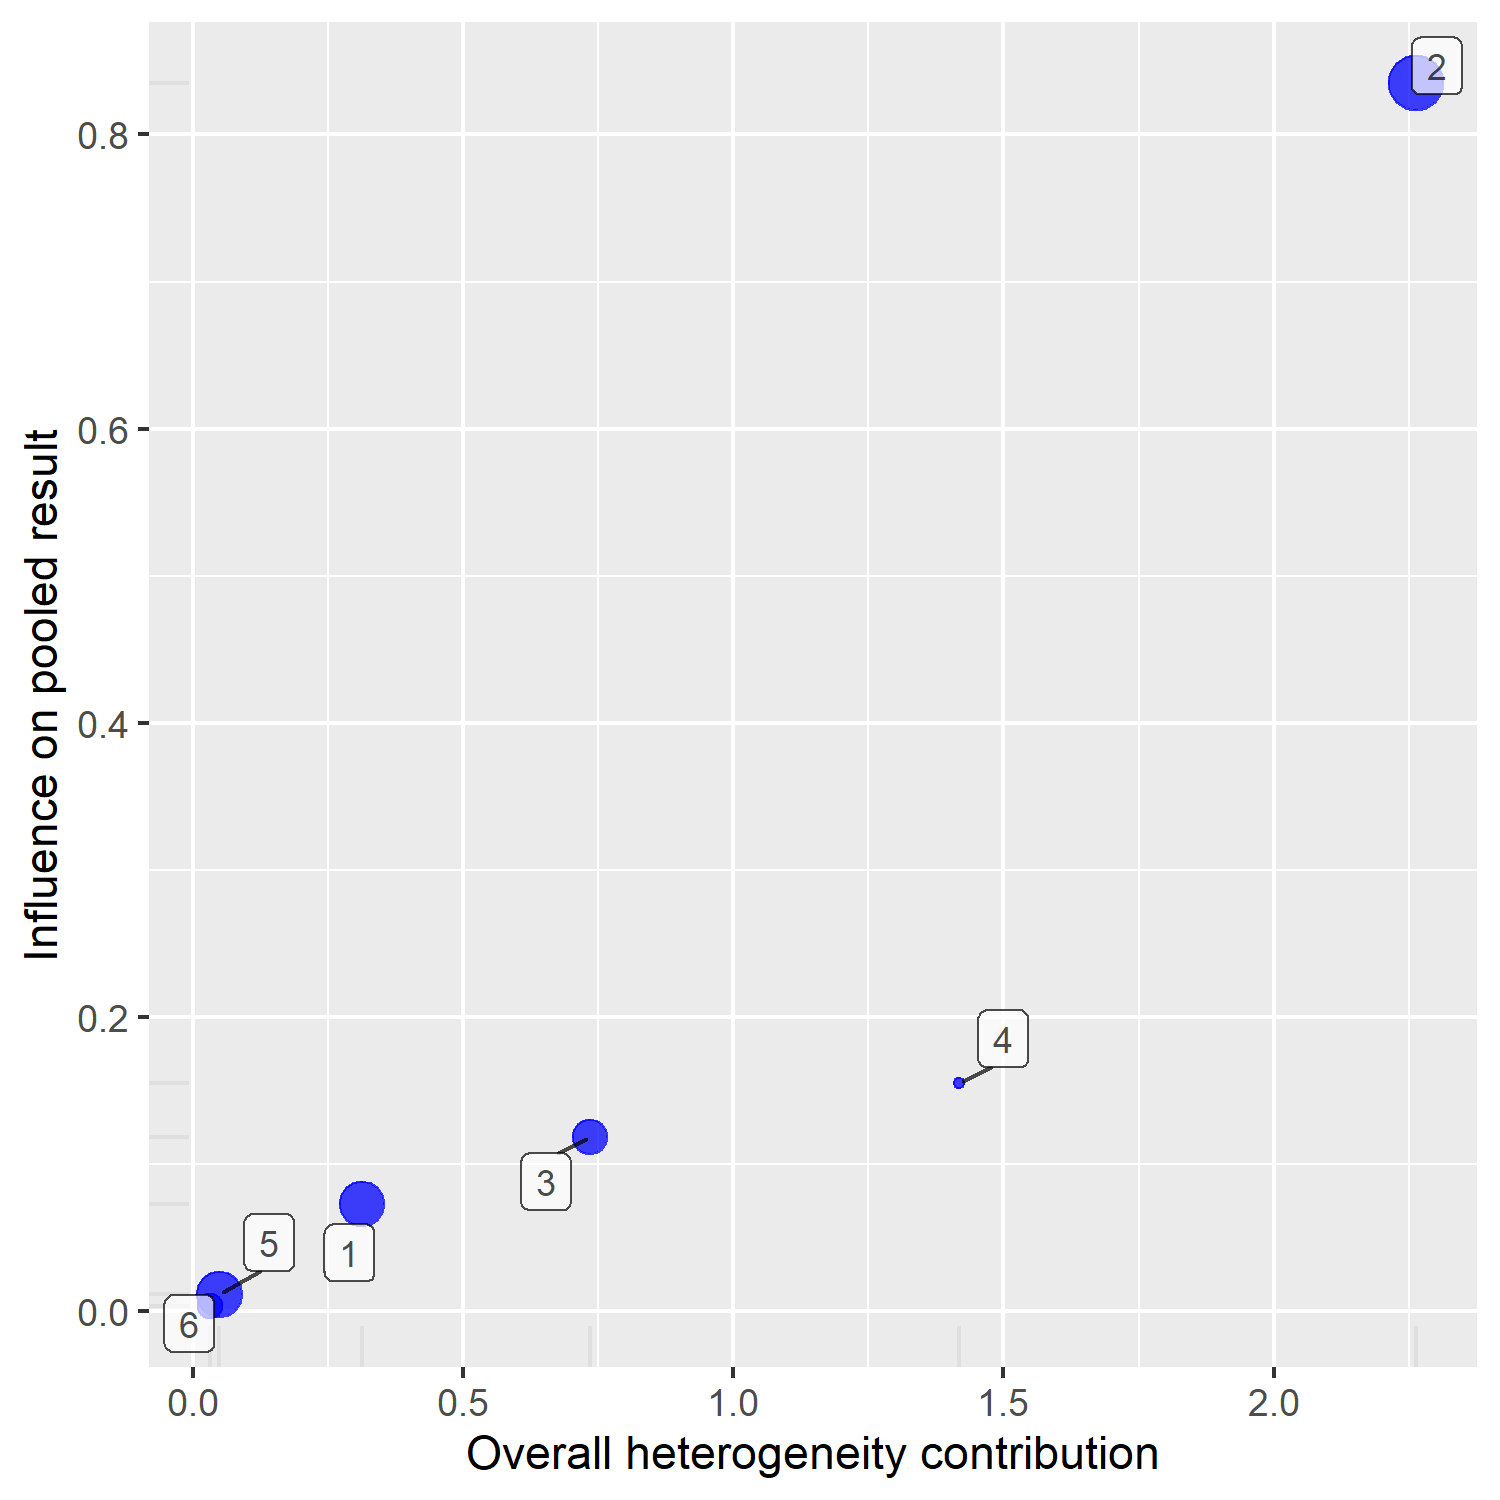
\includegraphics[width=0.5\linewidth]{figures/fig8} }

}

\caption{Baujat plots based on the leave-one-out method.}\label{fig:fig6}
\end{figure}

\hypertarget{discussion}{%
\section{Discussion}\label{discussion}}

The aim of this work was to evaluate the methodological quality of meta-analyses in tDCS-motor learning research with respect to reporting quality, reproducibility, and publication bias control. We found the meta-analyses we studied to be lacking in all three points. Although the meta-analyses reported the content of most PRISMA (Moher et al., 2009) items, they described their methods so sparsely as to render reproducing their procedure impossible without lengthy detective work. None of the meta-analyses had pre-registration protocols, shared their data, or provided their data-analysis code. We failed to numerically reproduce the main pooled ES estimates reported in all meta-analyses when following the procedures they described. As to publication bias control, only meta-analysis 3 reported having searched the grey literature and all three meta-analyses mostly used ``traditional'' publication bias detection and correction tools without discussion of their assumptions or appropriateness.

To give a more comprehensive account of our results, with respect to reporting quality as measured by adherence to PRISMA items, our findings mostly follow the pattern of those reported in Table 2. Concretely, similarly to the large sample of systematic reviews investigated by Page and Moher (2017), only meta-analysis 3 mentioned pre-registration (item 5), included a reproducible search string for a database (item 8), and conducted an assessment of bias in the individual studies (item 12). Notable differences between our sample and that of Page and Moher (2017) is that all three meta-analyses we reviewed included a list of variables they sought data for (item 11), conducted statistical assessments of bias across studies (items 15 and 22), and reported the results of their study selection procedure (item 17), although none of them described the actual procedure (item 9).

With respect to reproducibility, the most notable finding is probably the high prevalence of discrepancies between how the meta-analysts reported having computed individual ESs and how they really did it. These discrepancies were most often in relation to the outcomes used. For example, there were multiple cases where the meta-analysis reported having used an outcome X whereas they actually used the outcome change in X from baseline. This was particularly perplexing when values for both outcomes were reported in the primary study. In general, all primary studies included in the meta-analyses reported values/tests for several outcomes and meta-analysis 3 was the only one to provide a rationale, albeit a vague one\footnote{Namely that they used the outcome the respective primary study defined as their primary outcome.}, for why they chose the outcome they did for each primary study. In most cases, it was impossible to infer how these things came about as the authors of meta-analyses 1 and 2 did not respond to our request for data or data analysis code or protocol and the authors of meta-analysis 3 did not respond to our email at all. On the whole, we had similar difficulties in our reproducibility endeavour as Lakens et al. (2017) and Maassen et al. (2020).

However, although our reproduced pooled SMDs were calculated using less primary SMDs for all three meta-analyses (due to methodologically irreproducible SMDs), none of our reproductions led to a radical change in the pooled ES estimate like in Gøtzsche et al.'s (2007) or Ford et al.'s (2010) reviews. Indeed, our reproduced pooled SMDs for meta-analyses 1 and 2 were both significant in the same direction as the original ones, which is one of the many commonly used criteria for a successful replication (e.g., in large scale replication projects such as the one conducted by the Open Science Collaboration, 2015). This can be seen as an indication for inferential reproducibility of the meta-analyses' main conclusions, albeit a weak one, as this criterion for successful replication is often criticised and thus used in combination with other criteria (Heirene, 2021; Open Science Collaboration, 2015). A more thorough evaluation of inferential reproducibility would require a deeper dive into both methodological (e.g., marked differences in heterogeneity parameters between the reproduced and reported models) and tDCS-related aspects.

As to statistical publication bias analysis, like Banks, Kepes, and McDaniel (2012), we found the meta-analyses we reviewed to mostly use outdated publication bias control methods. However, this was not the critical issue, rather the fact the meta-analysts reported the results of their analyses very briefly and without discussion of their assumptions and their appropriateness for the data at hand. As mentioned before, publication bias testing remains an exceedingly active and contentious field of research and no consensus exists as of yet regarding which tests to use under which conditions. Any single test or constellation of tests used is thus inevitably arbitrary. One major problem all current methods suffer from is their mediocre performance when applied to a heterogeneous set of ESs. Meta-analyses 1 and 2 synthesised such sets of ESs, meta-analysis 3 only included 6 primary studies.

Furthermore, the primary studies included in the meta-analyses are likely to have been selected for publication based on different values than the ones the meta-analysts (and we) used for the publication bias tests (i.e., results of omnibus tests on several outcomes and not the pair-wise comparisons in one outcome at a single time point). This is especially relevant for the \(p\)-curve and the selection model we used of which an important step is dividing the set of ESs into significant and non-significant ones. Therefore, the results of both our and the meta-analysts' statistical publication bias tests can only be taken with a grain of salt. Nevertheless, the fact that all three meta-analysts used more than one tool is commendable as ``{[}a{]}ny assessment of publication bias is better than none, and using all methods available is better than using only one.'' (Vevea et al., 2019, p. 392). Their publication bias analysis would have been more informative had they used more recent methods as sensitivity analyses and provided clearer descriptions of the implications of tests' results.

Attempting to reproduce the meta-analyses revealed further methodological issues which do not directly pertain to the main methodological aspects we investigated: All three meta-analyses indiscriminately combined primary studies of different designs. For example, they computed SMDs using the same formula for both controlled and crossover designs, a procedure which neglects bias resulting from estimating sampling variances for crossover studies without accounting for carry-over effects or correlations between time points (Borenstein \& Hedges, 2019; Madeyski \& Kitchenham, 2018; Morris \& DeShon, 2002). Furthermore, the fact the meta-analysts used the total sample size of the cross-over trial to replace the treatment and control group sample sizes is likely to have inflated the power of these pair-wise comparisons (which is especially relevant for the publication bias tests). Another issue the meta-analysts neglected to account for is ES dependency (Gleser \& Olkin, 2009), which is especially critical in the case of the first two meta-analyses as they derived multiple ESs from single studies.

Moreover, although there are several ways to calculate an SMD besides the classic formula based on means and SDs (for an overview see Borenstein \& Hedges, 2019), it can be argued that the meta-analyses we reviewed used methods that went beyond what is plausible. For example, \(p\)-values based on median tests were used to calculate SMDs in two of the meta-analyses. Medians can replace means when they are derived from normally distributed data. However, primary studies usually report medians and interquartile ranges instead of means and SDs \emph{because} their samples are not normally distributed (Higgins et al., 2019, p. 167). This is likely to have been the case as most studies in the meta-analyses we reviewed are small. Besides, one would still need to impute the corresponding SDs. Similarly, Higgins et al. (2019) advise against combining SMDs based on post values and SMDs based on change from baseline as the SDs used to standardise them estimate different entities (p.~253).

All in all, our results indicate that the methodological limitations prevalent in meta-analyses in neighbouring fields can also be observed in meta-analyses studying the effect of tDCS on motor learning. This is unfortunate since together, the three meta-analyses have been cited over 200 times and knowing the high status meta-analyses enjoy on the ``hierarchy of evidence'' (Evans, 2003), they are likely to be influential beyond the restricted realm of scientific publishing. Naive consumers of these meta-analyses might be mislead into believing that they provide a definitive ``proof'' of the tDCS' effectiveness and researchers will have trouble evaluating the validity of the meta-analyses' methodology due to the rather limited reporting in key aspects (e.g., how and why studies and outcomes were selected) and the lack of pre-registered protocols, raw data or data analysis code (Page, McKenzie, et al., 2021; Page, Moher, et al., 2021).

Although the meta-analyses we reviewed were adequate in some aspects (e.g., description of outcome used for each primary study), there is clearly some room for improvement. As a remedy for the compromised reporting quality and reproducibility, more detailed descriptions of the methodological procedure are called for, ideally accompanied by raw data and the data analysis code (Page, Moher, et al., 2021). For publication bias assessment, a more extensive testing procedure involving sensitivity analyses both within a single method and across the different methods is necessary (following a literature search which is as comprehensive as allocated resources permit, Vevea et al., 2019). When dealing with a highly heterogeneous set of ESs, van Aert, Wicherts, and van Assen (2016) recommend splitting the set into subgroups based on theoretical and methodological considerations before carrying out the bias testing procedure. Inzlicht, Gervais, and Berkman (2015) recommend presenting a range of plausible pooled ESs based on different publication bias tests (using different assumptions).

No self-evident solutions can be offered for the shortcomings related to the computational aspects of the meta-analyses. There is immense variation in reporting quality of primary studies and meta-analysts usually have no other choice but to work with the data reported in the primary study (that is, when contacting the authors of the primary study for more data is not feasible or proves to be fruitless, Higgins et al., 2019). It is thus entirely understandable that meta-analysts must sometimes resort to alternative means of calculating certain measures. However, there \emph{are} limits to how divergent the alternative methods can be. For example, instead of converting a \(p\)-value derived from a medians test to an SMD, the meta-analysts could have estimated the means and SDs based on the medians and the corresponding ranges and or interquartile ranges calculated the SMD based on these means and SDs, which would have yielded a more comparable result to an SMD calculated on actual means and SDs (Hozo, Djulbegovic, \& Hozo, 2005; Wan, Wang, Liu, \& Tong, 2014).

Similarly, there are methods to compute the ESs and their corresponding sampling variances when dealing with crossover studies (Madeyski \& Kitchenham, 2018). Even estimating the ESs using the formula for within-subjects designs would have been better as these would have at least taken the correlations between time points, but not the carry-over effects, into account (Borenstein \& Hedges, 2019).
Instead of combining ESs derived from primary studies with different designs to compute a single pooled ESs, a practice strongly discouraged by meta-analysis pioneers like Borenstein and Hedges (2019) as such primary ESs cannot be seen as estimating the same parameter, meta-analysts can conduct multiple meta-analyses by grouping similar studies together. In some cases, meta-analysts must accept the loss of power by excluding primary studies, which are markedly different from the other studies in key aspects or which display a high or unclear risk of bias (Higgins et al., 2019, p. 192). Finally, it is paramount that the meta-analysts report how they computed each ES regardless of how they dealt with limited reporting in the primary study.

The fact that our publication bias testing routine is unlikely to have yielded more meaningful results than that of the meta-analysts is not the only limitation to our work. Others include:

\begin{itemize}
\tightlist
\item
  We have defined our exclusion criteria based on mostly practical considerations. Their high restrictiveness has probably led to a sample that is not representative of the field at large. Our non-systematic literature search and study selection strategy can only have exasperated this issue. It also goes without saying that three meta-analyses is too small a sample to draw far-reaching conclusions.
\item
  Although we had a mechanism in place to minimise the probability of data extraction errors on our part when evaluating reproducibility, it cannot be excluded that potential errors when extracting data for other variables (e.g., for PRISMA adherence) influenced our results as data extraction and coding was not checked by others (Buscemi, Hartling, Vandermeer, Tjosvold, \& Klassen, 2006; Jones, Remmington, Williamson, Ashby, \& Smyth, 2005).
\item
  We focused on reproducibility of data extraction and calculation of ESs because previous reviews demonstrated a high prevalence of mistakes in these steps. However, it cannot be excluded that other aspects we neglected such as study search and selection have a larger impact.
\item
  Throughout the process of reproduction, we had to make subjective decisions that cannot be guaranteed to have been faultless. Notably, it was not always trivial to judge whether our procedure for reproducing a certain primary SMD strictly followed the procedure purported to have been used by the meta-analysts. For example, we managed to approximate SMD no. 5 in meta-analysis 3 by averaging the means and SDs of two outcomes and computing an SMDs based on the average value. We subsequently classified this SMD as faithfully reproducible because the meta-analysts reported having used what each primary study defined as its primary outcome and this specific primary study defined both these outcomes as its primary outcomes. However, since the meta-analysts did not provide any information on how they computed the SMD or any indication that they took an average, it is almost certain that they calculated the SMD differently because otherwise we would have successfully reproduced the SMD to the third decimal like we did the other brute-force reproducible ones. Other such examples are documented in the data analysis notebook.
\item
  Due to our rather limited expertise with regards to the technical and practical aspects of tDCS research, it cannot be excluded that we have overlooked or misunderstood relevant tDCS-related methodological facets.
\end{itemize}

Future similar works may thus aim for a more fine-grained and nuanced evaluation of reporting quality which goes beyond the minimal requirements set by reporting guidelines, a more comprehensive reproducibility testing which is not restricted to data extraction and ES calculation as well as a thorough investigation of robustness towards changes in analytical decisions (especially data selection and outcomes used), and a more principled approach towards evaluating publication bias assessment.

Despite these limitations, we hope to have provided consumers of tDCS-motor learning research with an incentive to evaluate meta-analyses in this field more critically when making decisions about the use of tDCS and meta-analysts with aspects to consider when conducting meta-analyses in the future. By no means do we want to imply that the solutions presented above are easy. Despite the abundance and comprehensiveness of guidelines such as PRISMA and tutorials on how to conduct a transparent and reproducible meta-analysis (e.g., Moreau \& Gamble, 2020; Quintana, 2015), it is undeniable that meticulous adherence to guidelines and making one's meta-analysis reproducible require a substantial amount of time and effort. Likewise, it cannot be expected from substantive researchers to be adept at every methodological/statistical aspect relevant to conducting a meta-analysis. A discussion of potential measures to improve the situation on a higher, more structural level, such as ways to incentivise transparency-related practices (Bakker, van Dijk, \& Wicherts, 2012; Higginson \& Munafò, 2016; B. A. Nosek et al., 2015) or journals employing specialised statistical review (Hardwicke, Frank, Vazire, \& Goodman, 2019), is beyond the scope of this work.

Nevertheless, given the epistemic weight meta-analyses usually carry, problems associated with how they are conducted and reported cannot be shrugged off. Efforts to improve them should be promoted. Besides the guidelines which are constantly being updated and advancements in statistical procedures for controlling publication bias, many methodological procedures have been developed in the recent years to systematically account for the impact of different analytical decisions (Taylor \& Munafò, 2016; e.g., Voracek et al., 2019). More emphasis is also being placed on flagship open science practices such as pre-registration and data and code sharing (Maassen et al., 2020; Page, Moher, et al., 2021).

Finally, since meta-analyses can only be as good as the primary literatures they synthesise, meta-analysts cannot be expected to carry all the responsibility for improvement {[}Aguinis, Pierce, et al. (2011); Borenstein et al. (2009b). In the quest for a reliable cumulative science, efforts to counteract the methodological issues found in the tDCS primary literature (e.g., heterogeneity in employed tDCS parameters, compromised reproducibility due to incomplete reporting Buch et al., 2017) must also be supported. Such efforts include mathematical models which can be used to systematically determine the optimal tDCS parameters to use (Lipka et al., 2021) and checklists outlining all aspects which should be disclosed when reporting the results of a tDCS study (Buch et al., 2017).

\newpage

\hypertarget{references}{%
\section{References}\label{references}}

\begingroup
\setlength{\parindent}{-0.5in}

\hypertarget{refs}{}
\begin{CSLReferences}{1}{0}
\leavevmode\vadjust pre{\hypertarget{ref-adaImpactMetaanalyticDecisions2012a}{}}%
Ada, S., Sharman, R., \& Balkundi, P. (2012). Impact of meta-analytic decisions on the conclusions drawn on the business value of information technology. \emph{Decision Support Systems}, \emph{54}(1), 521--533. \url{https://doi.org/10.1016/j.dss.2012.07.001}

\leavevmode\vadjust pre{\hypertarget{ref-aguinisMetaAnalyticChoicesJudgment2011}{}}%
Aguinis, H., Dalton, D. R., Bosco, F. A., Pierce, C. A., \& Dalton, C. M. (2011). Meta-{Analytic Choices} and {Judgment Calls}: {Implications} for {Theory Building} and {Testing}, {Obtained Effect Sizes}, and {Scholarly Impact}. \emph{Journal of Management}, \emph{37}(1), 5--38. \url{https://doi.org/10.1177/0149206310377113}

\leavevmode\vadjust pre{\hypertarget{ref-aguinisDebunkingMythsUrban2011}{}}%
Aguinis, H., Pierce, C. A., Bosco, F. A., Dalton, D. R., \& Dalton, C. M. (2011). Debunking {Myths} and {Urban Legends About Meta-Analysis}. \emph{Organizational Research Methods}, \emph{14}(2), 306--331. \url{https://doi.org/10.1177/1094428110375720}

\leavevmode\vadjust pre{\hypertarget{ref-ahnReviewMetaAnalysesEducation2012}{}}%
Ahn, S., Ames, A. J., \& Myers, N. D. (2012). A {Review} of {Meta-Analyses} in {Education}: {Methodological Strengths} and {Weaknesses}. \emph{Review of Educational Research}, \emph{82}(4), 436--476. \url{https://doi.org/10.3102/0034654312458162}

\leavevmode\vadjust pre{\hypertarget{ref-R-papaja}{}}%
Aust, F., \& Barth, M. (2020). \emph{Papaja: {Create APA} manuscripts with {R Markdown}} {[}Manual{]}.

\leavevmode\vadjust pre{\hypertarget{ref-austinPrefrontalElectricalStimulation2016}{}}%
Austin, A., Jiga-Boy, G. M., Rea, S., Newstead, S. A., Roderick, S., Davis, N. J., \ldots{} Boy, F. (2016). Prefrontal {Electrical Stimulation} in {Non-depressed Reduces Levels} of {Reported Negative Affects} from {Daily Stressors}. \emph{Frontiers in Psychology}, \emph{7}, 315. \url{https://doi.org/10.3389/fpsyg.2016.00315}

\leavevmode\vadjust pre{\hypertarget{ref-aytugRevealedConcealedTransparency2012}{}}%
Aytug, Z. G., Rothstein, H. R., Zhou, W., \& Kern, M. C. (2012). Revealed or {Concealed}? {Transparency} of {Procedures}, {Decisions}, and {Judgment Calls} in {Meta-Analyses}. \emph{Organizational Research Methods}, \emph{15}(1), 103--133. \url{https://doi.org/10.1177/1094428111403495}

\leavevmode\vadjust pre{\hypertarget{ref-bakkerRulesGameCalled2012}{}}%
Bakker, M., van Dijk, A., \& Wicherts, J. M. (2012). The {Rules} of the {Game Called Psychological Science}. \emph{Perspectives on Psychological Science}, \emph{7}(6), 543--554. \url{https://doi.org/10.1177/1745691612459060}

\leavevmode\vadjust pre{\hypertarget{ref-R-meta}{}}%
Balduzzi, S., Rücker, G., \& Schwarzer, G. (2019). How to perform a meta-analysis with {R}: A practical tutorial. \emph{Evidence-Based Mental Health}, (22), 153--160.

\leavevmode\vadjust pre{\hypertarget{ref-banksPublicationBiasCall2012}{}}%
Banks, G. C., Kepes, S., \& McDaniel, M. A. (2012). Publication {Bias}: {A} call for improved meta-analytic practice in the organizational sciences. \emph{International Journal of Selection and Assessment}, \emph{20}(2), 182--196. \url{https://doi.org/10.1111/j.1468-2389.2012.00591.x}

\leavevmode\vadjust pre{\hypertarget{ref-R-Matrix}{}}%
Bates, D., \& Maechler, M. (2021). \emph{Matrix: {Sparse} and dense matrix classes and methods} {[}Manual{]}.

\leavevmode\vadjust pre{\hypertarget{ref-beggOperatingCharacteristicsRank1994}{}}%
Begg, C. B., \& Mazumdar, M. (1994). Operating characteristics of a rank correlation test for publication bias. \emph{Biometrics}, 1088--1101.

\leavevmode\vadjust pre{\hypertarget{ref-bennabiTranscranialDirectCurrent2014}{}}%
Bennabi, D., Pedron, S., Haffen, E., Monnin, J., Peterschmitt, Y., \& Van Waes, V. (2014). Transcranial direct current stimulation for memory enhancement: From clinical research to animal models. \emph{Frontiers in Systems Neuroscience}, \emph{8}, 159. \url{https://doi.org/10.3389/fnsys.2014.00159}

\leavevmode\vadjust pre{\hypertarget{ref-borensteinEffectSizesMetaanalyses2019}{}}%
Borenstein, M., \& Hedges, L. V. (2019). Effect sizes for meta-analyses. In \emph{The {Handbook} of {Research Synthesis} and {Meta-Analysis},} (pp. 207--241).

\leavevmode\vadjust pre{\hypertarget{ref-borensteinPublicationBias2009}{}}%
Borenstein, M., Hedges, L. V., Higgins, J. P. T., \& Rothstein, H. R. (2009a). Publication {Bias}. In \emph{Introduction to {Meta-Analysis}} (pp. 277--292). {John Wiley \& Sons, Ltd}. \url{https://doi.org/10.1002/9780470743386.ch30}

\leavevmode\vadjust pre{\hypertarget{ref-borensteinCriticismsMetaanalysis2009}{}}%
Borenstein, M., Hedges, L., Higgins, J. P. T., \& Rothstein, H. R. (2009b). Criticisms of meta-analysis. In \emph{Introduction to {Meta-Analysis}} (pp. 377--387).

\leavevmode\vadjust pre{\hypertarget{ref-botvinik-nezerVariabilityAnalysisSingle2020}{}}%
Botvinik-Nezer, R., Holzmeister, F., Camerer, C. F., Dreber, A., Huber, J., Johannesson, M., \ldots{} Schonberg, T. (2020). Variability in the analysis of a single neuroimaging dataset by many teams. \emph{Nature}, \emph{582}(7810), 84--88. \url{https://doi.org/10.1038/s41586-020-2314-9}

\leavevmode\vadjust pre{\hypertarget{ref-bromanRecommendationsFundingAgencies2017}{}}%
Broman, K., Cetinkaya-Rundel, M., Nussbaum, A., Paciorek, C., Peng, R., Turek, D., \& Wickham, H. (2017). \emph{Recommendations to {Funding Agencies} for {Supporting Reproducible Research}}.

\leavevmode\vadjust pre{\hypertarget{ref-brunoniTranscranialDirectCurrent2016}{}}%
Brunoni, A. R., Moffa, A. H., Fregni, F., Palm, U., Padberg, F., Blumberger, D. M., \ldots{} Loo, C. K. (2016). Transcranial direct current stimulation for acute major depressive episodes: Meta-analysis of individual patient data. \emph{The British Journal of Psychiatry}, \emph{208}(6), 522--531. \url{https://doi.org/10.1192/bjp.bp.115.164715}

\leavevmode\vadjust pre{\hypertarget{ref-buchEffectsTDCSMotor2017}{}}%
Buch, E. R., Santarnecchi, E., Antal, A., Born, J., Celnik, P. A., Classen, J., \ldots{} Cohen, L. G. (2017). Effects of {tDCS} on motor learning and memory formation: {A} consensus and critical position paper. \emph{Clinical Neurophysiology}, \emph{128}(4), 589--603. \url{https://doi.org/10.1016/j.clinph.2017.01.004}

\leavevmode\vadjust pre{\hypertarget{ref-buscemiSingleDataExtraction2006}{}}%
Buscemi, N., Hartling, L., Vandermeer, B., Tjosvold, L., \& Klassen, T. P. (2006). Single data extraction generated more errors than double data extraction in systematic reviews. \emph{Journal of Clinical Epidemiology}, \emph{59}(7), 697--703. \url{https://doi.org/10.1016/j.jclinepi.2005.11.010}

\leavevmode\vadjust pre{\hypertarget{ref-buttonPowerFailureWhy2013}{}}%
Button, K. S., Ioannidis, J. P. A., Mokrysz, C., Nosek, B. A., Flint, J., Robinson, E. S. J., \& Munafò, M. R. (2013). Power failure: Why small sample size undermines the reliability of neuroscience. \emph{Nature Reviews Neuroscience}, \emph{14}(5), 365--376. \url{https://doi.org/10.1038/nrn3475}

\leavevmode\vadjust pre{\hypertarget{ref-carterCorrectingBiasPsychology2019}{}}%
Carter, E. C., Schönbrodt, F. D., Gervais, W. M., \& Hilgard, J. (2019). Correcting for {Bias} in {Psychology}: {A Comparison} of {Meta-Analytic Methods}. \emph{Advances in Methods and Practices in Psychological Science}, \emph{2}(2), 115--144. \url{https://doi.org/10.1177/2515245919847196}

\leavevmode\vadjust pre{\hypertarget{ref-cooperHandbookResearchSynthesis2009}{}}%
Cooper, H., Hedges, L. V., \& Valentine, J. C. (Eds.). (2009). \emph{The {Handbook} of {Research Synthesis} and {Meta-Analysis}} (2nd edition). {New York}: {Russell Sage Foundation}.

\leavevmode\vadjust pre{\hypertarget{ref-davisRegulationConsumerTDCS2016}{}}%
Davis, N. J. (2016). The regulation of consumer {tDCS}: Engaging a community of creative self-experimenters. \emph{JL \& Biosciences}, \emph{3}, 304.

\leavevmode\vadjust pre{\hypertarget{ref-dersimonianMetaanalysisClinicalTrials1986}{}}%
DerSimonian, R., \& Laird, N. (1986). Meta-analysis in clinical trials. \emph{Controlled Clinical Trials}, \emph{7}(3), 177--188.

\leavevmode\vadjust pre{\hypertarget{ref-dieckmannEmpiricalAssessmentMetaAnalytic2009}{}}%
Dieckmann, N. F., Malle, B. F., \& Bodner, T. E. (2009). An {Empirical Assessment} of {Meta-Analytic Practice}. \emph{Review of General Psychology}, \emph{13}(2), 101--115. \url{https://doi.org/10.1037/a0015107}

\leavevmode\vadjust pre{\hypertarget{ref-dubljevicRisingTideTDCS2014}{}}%
Dubljević, V., Saigle, V., \& Racine, E. (2014). The {Rising Tide} of {tDCS} in the {Media} and {Academic Literature}. \emph{Neuron}, \emph{82}(4), 731--736. \url{https://doi.org/10.1016/j.neuron.2014.05.003}

\leavevmode\vadjust pre{\hypertarget{ref-duvalNonparametricTrimFill2000}{}}%
Duval, S., \& Tweedie, R. (2000a). A {Nonparametric} "{Trim} and {Fill}" {Method} of {Accounting} for {Publication Bias} in {Meta-Analysis}. \emph{Journal of the American Statistical Association}, \emph{95}(449), 89--98. \url{https://doi.org/10.2307/2669529}

\leavevmode\vadjust pre{\hypertarget{ref-duvalTrimFillSimple2000}{}}%
Duval, S., \& Tweedie, R. (2000b). Trim and {Fill}: {A Simple Funnel-Plot}\textendash{{Based Method}} of {Testing} and {Adjusting} for {Publication Bias} in {Meta-Analysis}. \emph{Biometrics}, \emph{56}(2), 455--463. \url{https://doi.org/10.1111/j.0006-341X.2000.00455.x}

\leavevmode\vadjust pre{\hypertarget{ref-eggerBiasMetaanalysisDetected1997}{}}%
Egger, M., Smith, G. D., Schneider, M., \& Minder, C. (1997). Bias in meta-analysis detected by a simple, graphical test. \emph{BMJ}, \emph{315}(7109), 629--634. \url{https://doi.org/10.1136/bmj.315.7109.629}

\leavevmode\vadjust pre{\hypertarget{ref-evansHierarchyEvidenceFramework2003}{}}%
Evans, D. (2003). Hierarchy of evidence: A framework for ranking evidence evaluating healthcare interventions. \emph{Journal of Clinical Nursing}, \emph{12}(1), 77--84. \url{https://doi.org/10.1046/j.1365-2702.2003.00662.x}

\leavevmode\vadjust pre{\hypertarget{ref-fanelliPositiveResultsIncrease2010}{}}%
Fanelli, D. (2010). {``{Positive}''} {Results Increase Down} the {Hierarchy} of the {Sciences}. \emph{PLOS ONE}, \emph{5}(4), e10068. \url{https://doi.org/10.1371/journal.pone.0010068}

\leavevmode\vadjust pre{\hypertarget{ref-fordErrorsConductSystematic2010}{}}%
Ford, A. C., Guyatt, G. H., Talley, N. J., \& Moayyedi, P. (2010). Errors in the conduct of systematic reviews of pharmacological interventions for irritable bowel syndrome. \emph{The American Journal of Gastroenterology}, \emph{105}(2), 280--288. \url{https://doi.org/10.1038/ajg.2009.658}

\leavevmode\vadjust pre{\hypertarget{ref-fregniRegulatoryConsiderationsClinical2015}{}}%
Fregni, F., Nitsche, M. A., Loo, C. K., Brunoni, A. R., Marangolo, P., Leite, J., \ldots{} Bikson, M. (2015). Regulatory {Considerations} for the {Clinical} and {Research Use} of {Transcranial Direct Current Stimulation} ({tDCS}): Review and recommendations from an expert panel. \emph{Clinical Research and Regulatory Affairs}, \emph{32}(1), 22--35. \url{https://doi.org/10.3109/10601333.2015.980944}

\leavevmode\vadjust pre{\hypertarget{ref-friesePHackingPublicationBias2020}{}}%
Friese, M., \& Frankenbach, J. (2020). P-{Hacking} and publication bias interact to distort meta-analytic effect size estimates. \emph{Psychological Methods}, \emph{25}(4), 456--471. \url{https://doi.org/10.1037/met0000246}

\leavevmode\vadjust pre{\hypertarget{ref-gazzanigaMethodsCognitiveNeuroscience2018}{}}%
Gazzaniga, M., Ivry, R. B., \& Mangun, G. R. (2018). Methods of {Cognitive Neuroscience}. In \emph{Cognitive {Neuroscience}: {The Biology} of the {Mind}} (Fifth edition). {New York}: {W. W. Norton \& Company}.

\leavevmode\vadjust pre{\hypertarget{ref-gebodhTranscranialDirectCurrent2019}{}}%
Gebodh, N., Esmaeilpour, Z., Adair, D., Schestattsky, P., Fregni, F., \& Bikson, M. (2019). Transcranial {Direct Current Stimulation Among Technologies} for {Low-Intensity Transcranial Electrical Stimulation}: {Classification}, {History}, and {Terminology}. In H. Knotkova, M. A. Nitsche, M. Bikson, \& A. J. Woods (Eds.), \emph{Practical {Guide} to {Transcranial Direct Current Stimulation}: {Principles}, {Procedures} and {Applications}} (pp. 3--43). {Cham}: {Springer International Publishing}. \url{https://doi.org/10.1007/978-3-319-95948-1_1}

\leavevmode\vadjust pre{\hypertarget{ref-gelmanGardenForkingPaths2013}{}}%
Gelman, A., \& Loken, E. (2013). The garden of forking paths: {Why} multiple comparisons can be a problem, even when there is no {``fishing expedition''} or {``p-hacking''} and the research hypothesis was posited ahead of time. \emph{Department of Statistics, Columbia University}, \emph{348}.

\leavevmode\vadjust pre{\hypertarget{ref-geyskensReviewEvaluationMetaAnalysis2009}{}}%
Geyskens, I., Krishnan, R., Steenkamp, J.-B. E. M., \& Cunha, P. V. (2009). A {Review} and {Evaluation} of {Meta-Analysis Practices} in {Management Research}. \emph{Journal of Management}, \emph{35}(2), 393--419. \url{https://doi.org/10.1177/0149206308328501}

\leavevmode\vadjust pre{\hypertarget{ref-gianniTDCSRandomizedControlled2021}{}}%
Gianni, E., Bertoli, M., Simonelli, I., Paulon, L., Tecchio, F., \& Pasqualetti, P. (2021). {tDCS} randomized controlled trials in no-structural diseases: A quantitative review. \emph{Scientific Reports}, \emph{11}(1), 16311. \url{https://doi.org/10.1038/s41598-021-95084-6}

\leavevmode\vadjust pre{\hypertarget{ref-gleserStochasticallyDependentEffect2009}{}}%
Gleser, L. J., \& Olkin, I. (2009). Stochastically dependent effect sizes. In \emph{The handbook of research synthesis and meta-analysis, 2nd ed} (pp. 357--376). {New York, NY, US}: {Russell Sage Foundation}.

\leavevmode\vadjust pre{\hypertarget{ref-goodmanWhatDoesResearch2016}{}}%
Goodman, S. N., Fanelli, D., \& Ioannidis, J. P. A. (2016). What does research reproducibility mean? \emph{Science Translational Medicine}, \emph{8}(341), 341ps12. \url{https://doi.org/10.1126/scitranslmed.aaf5027}

\leavevmode\vadjust pre{\hypertarget{ref-gopalakrishnanSystematicReviewsMetaanalysis2013}{}}%
Gopalakrishnan, S., \& Ganeshkumar, P. (2013). Systematic {Reviews} and {Meta-analysis}: {Understanding} the {Best Evidence} in {Primary Healthcare}. \emph{Journal of Family Medicine and Primary Care}, \emph{2}(1), 9--14. \url{https://doi.org/10.4103/2249-4863.109934}

\leavevmode\vadjust pre{\hypertarget{ref-gotzscheDataExtractionErrors2007}{}}%
Gøtzsche, P. C., Hróbjartsson, A., Marić, K., \& Tendal, B. (2007). Data {Extraction Errors} in {Meta-analyses That Use Standardized Mean Differences}. \emph{JAMA}, \emph{298}(4), 430--437. \url{https://doi.org/10.1001/jama.298.4.430}

\leavevmode\vadjust pre{\hypertarget{ref-guzzoMetaanalysisAnalysis1987}{}}%
Guzzo, R., Jackson, S., \& Katzell, R. (1987). Meta-analysis analysis. \emph{Undefined}.

\leavevmode\vadjust pre{\hypertarget{ref-hardwickeShouldPsychologyJournals2019}{}}%
Hardwicke, T. E., Frank, M. C., Vazire, S., \& Goodman, S. N. (2019). Should {Psychology Journals Adopt Specialized Statistical Review}? \emph{Advances in Methods and Practices in Psychological Science}, \emph{2}(3), 240--249. \url{https://doi.org/10.1177/2515245919858428}

\leavevmode\vadjust pre{\hypertarget{ref-harrerDoingMetaAnalysisHandsOn2021}{}}%
Harrer, M., Cuijpers, P., Furukawa, T. A., \& Ebert, D. D. (2021). \emph{Doing {Meta-Analysis With R}: {A Hands-On Guide}} (1st ed.). {Boca Raton, FL and London}: {Chapman \& Hall/CRC Press}.

\leavevmode\vadjust pre{\hypertarget{ref-R-dmetar}{}}%
Harrer, M., Cuijpers, P., Furukawa, T., \& Ebert, D. D. (2019). \emph{Dmetar: {Companion} r package for the guide 'doing meta-analysis in r'} {[}Manual{]}.

\leavevmode\vadjust pre{\hypertarget{ref-heireneCallReplicationsAddiction2021}{}}%
Heirene, R. M. (2021). A call for replications of addiction research: Which studies should we replicate and what constitutes a {``successful''} replication? \emph{Addiction Research \& Theory}, \emph{29}(2), 89--97. \url{https://doi.org/10.1080/16066359.2020.1751130}

\leavevmode\vadjust pre{\hypertarget{ref-R-purrr}{}}%
Henry, L., \& Wickham, H. (2020). \emph{Purrr: {Functional} programming tools} {[}Manual{]}.

\leavevmode\vadjust pre{\hypertarget{ref-higginsCochraneHandbookSystematic2019}{}}%
Higgins, J. P., Thomas, J., Chandler, J., Cumpston, M., Li, T., Page, M. J., \& Welch, V. A. (2019). \emph{Cochrane handbook for systematic reviews of interventions}. {John Wiley \& Sons}.

\leavevmode\vadjust pre{\hypertarget{ref-higginsonCurrentIncentivesScientists2016}{}}%
Higginson, A. D., \& Munafò, M. R. (2016). Current {Incentives} for {Scientists Lead} to {Underpowered Studies} with {Erroneous Conclusions}. \emph{PLOS Biology}, \emph{14}(11), e2000995. \url{https://doi.org/10.1371/journal.pbio.2000995}

\leavevmode\vadjust pre{\hypertarget{ref-hilgardOverstatedEvidenceShortterm2017}{}}%
Hilgard, J., Engelhardt, C. R., \& Rouder, J. N. (2017). \emph{Overstated evidence for short-term effects of violent games on affect and behavior: {A} reanalysis of {Anderson} et al.(2010).}

\leavevmode\vadjust pre{\hypertarget{ref-hohnEmpiricalReviewResearch2020}{}}%
Hohn, R. E., Slaney, K. L., \& Tafreshi, D. (2020). An {Empirical Review} of {Research} and {Reporting Practices} in {Psychological Meta-Analyses}. \emph{Review of General Psychology}, \emph{24}(3), 195--209. \url{https://doi.org/10.1177/1089268020918844}

\leavevmode\vadjust pre{\hypertarget{ref-horvathQuantitativeReviewFinds2015}{}}%
Horvath, J. C., Forte, J. D., \& Carter, O. (2015). Quantitative {Review Finds No Evidence} of {Cognitive Effects} in {Healthy Populations From Single-session Transcranial Direct Current Stimulation} ({tDCS}). \emph{Brain Stimulation}, \emph{8}(3), 535--550. \url{https://doi.org/10.1016/j.brs.2015.01.400}

\leavevmode\vadjust pre{\hypertarget{ref-R-MAd}{}}%
Hoyt, A. C. D. R. \&. W. T. (2014). \emph{{MAd}: {Meta-analysis} with mean differences} {[}Manual{]}.

\leavevmode\vadjust pre{\hypertarget{ref-hozoEstimatingMeanVariance2005}{}}%
Hozo, S. P., Djulbegovic, B., \& Hozo, I. (2005). Estimating the mean and variance from the median, range, and the size of a sample. \emph{BMC Medical Research Methodology}, \emph{5}(1), 13. \url{https://doi.org/10.1186/1471-2288-5-13}

\leavevmode\vadjust pre{\hypertarget{ref-hungEfficacyTranscranialDirect2021}{}}%
Hung, C.-M., Zeng, B.-Y., Zeng, B.-S., Sun, C.-K., Cheng, Y.-S., Su, K.-P., \ldots{} Tseng, P.-T. (2021b). The {Efficacy} of {Transcranial Direct Current Stimulation} in {Enhancing Surgical Skill Acquisition}: {A Preliminary Meta-Analysis} of {Randomized Controlled Trials}. \emph{Brain Sciences}, \emph{11}(6), 707. \url{https://doi.org/10.3390/brainsci11060707}

\leavevmode\vadjust pre{\hypertarget{ref-hungEfficacyTranscranialDirect2021a}{}}%
Hung, C.-M., Zeng, B.-Y., Zeng, B.-S., Sun, C.-K., Cheng, Y.-S., Su, K.-P., \ldots{} Tseng, P.-T. (2021a). The {Efficacy} of {Transcranial Direct Current Stimulation} in {Enhancing Surgical Skill Acquisition}: {A Preliminary Meta-Analysis} of {Randomized Controlled Trials}. \emph{Brain Sciences}, \emph{11}(6), 707. \url{https://doi.org/10.3390/brainsci11060707}

\leavevmode\vadjust pre{\hypertarget{ref-hyattQuandaryCovaryingBrief2020a}{}}%
Hyatt, C. S., Owens, M. M., Crowe, M. L., Carter, N. T., Lynam, D. R., \& Miller, J. D. (2020). The quandary of covarying: {A} brief review and empirical examination of covariate use in structural neuroimaging studies on psychological variables. \emph{NeuroImage}, \emph{205}, 116225. \url{https://doi.org/10.1016/j.neuroimage.2019.116225}

\leavevmode\vadjust pre{\hypertarget{ref-inzlichtBiasCorrectionTechniquesAlone2015}{}}%
Inzlicht, M., Gervais, W., \& Berkman, E. (2015). \emph{Bias-{Correction Techniques Alone Cannot Determine Whether Ego Depletion} is {Different} from {Zero}: {Commentary} on {Carter}, {Kofler}, {Forster}, \& {McCullough}, 2015}. \url{https://doi.org/10.2139/ssrn.2659409}

\leavevmode\vadjust pre{\hypertarget{ref-ioannidisMassProductionRedundant2016}{}}%
Ioannidis, J. P. A. (2016). The {Mass Production} of {Redundant}, {Misleading}, and {Conflicted Systematic Reviews} and {Meta-analyses}. \emph{The Milbank Quarterly}, \emph{94}(3), 485--514. \url{https://doi.org/10.1111/1468-0009.12210}

\leavevmode\vadjust pre{\hypertarget{ref-jonesHighPrevalenceLow2005}{}}%
Jones, A. P., Remmington, T., Williamson, P. R., Ashby, D., \& Smyth, R. L. (2005). High prevalence but low impact of data extraction and reporting errors were found in {Cochrane} systematic reviews. \emph{Journal of Clinical Epidemiology}, \emph{58}(7), 741--742. \url{https://doi.org/10.1016/j.jclinepi.2004.11.024}

\leavevmode\vadjust pre{\hypertarget{ref-kangTranscranialDirectCurrent2016a}{}}%
Kang, N., Summers, J. J., \& Cauraugh, J. H. (2016). Transcranial direct current stimulation facilitates motor learning post-stroke: A systematic review and meta-analysis. \emph{Journal of Neurology, Neurosurgery \& Psychiatry}, \emph{87}(4), 345--355. \url{https://doi.org/f8fwd8}

\leavevmode\vadjust pre{\hypertarget{ref-kangTranscranialDirectCurrent2018}{}}%
Kang, N., Weingart, A., \& Cauraugh, J. H. (2018). Transcranial direct current stimulation and suppression of contralesional primary motor cortex post-stroke: A systematic review and meta-analysis. \emph{Brain Injury}, \emph{32}(9), 1063--1070. \url{https://doi.org/10.1080/02699052.2018.1481526}

\leavevmode\vadjust pre{\hypertarget{ref-kepesMetaanalyticReviewsOrganizational2013}{}}%
Kepes, S., McDaniel, M. A., Brannick, M. T., \& Banks, G. C. (2013). Meta-analytic {Reviews} in the {Organizational Sciences}: {Two Meta-analytic Schools} on the {Way} to {MARS} (the {Meta-analytic Reporting Standards}). \emph{Journal of Business and Psychology}, \emph{28}(2), 123--143. \url{https://doi.org/10.1007/s10869-013-9300-2}

\leavevmode\vadjust pre{\hypertarget{ref-konstantopoulosStatisticallyAnalyzingEffect2019}{}}%
Konstantopoulos, S., \& Hedges, L. V. (2019). Statistically analyzing effect sizes: {Fixed-and} random-effects models. In \emph{The {Handbook} of {Research Synthesis} and {Meta-Analysis},} (pp. 245--279).

\leavevmode\vadjust pre{\hypertarget{ref-lakensExaminingReproducibilityMetaAnalyses2017}{}}%
Lakens, D., Page-Gould, E., Assen, M. A. L. M. van, Spellman, B., Schönbrodt, F., Hasselman, F., \ldots{} Scheel, A. M. (2017). \emph{Examining the {Reproducibility} of {Meta-Analyses} in {Psychology}: {A Preliminary Report}}. \url{https://doi.org/10.31222/osf.io/xfbjf}

\leavevmode\vadjust pre{\hypertarget{ref-liberatiPRISMAStatementReporting2009}{}}%
Liberati, A., Altman, D. G., Tetzlaff, J., Mulrow, C., Gøtzsche, P. C., Ioannidis, J. P. A., \ldots{} Moher, D. (2009). The {PRISMA} statement for reporting systematic reviews and meta-analyses of studies that evaluate healthcare interventions: Explanation and elaboration. \emph{BMJ}, \emph{339}, b2700. \url{https://doi.org/10.1136/bmj.b2700}

\leavevmode\vadjust pre{\hypertarget{ref-lightSummingScienceReviewing1984}{}}%
Light, R. J., \& Pillemer, D. B. (1984). \emph{Summing {Up}: {The Science} of {Reviewing Research}}. {Harvard University Press}.

\leavevmode\vadjust pre{\hypertarget{ref-lipkaResolvingHeterogeneityTranscranial2021}{}}%
Lipka, R., Ahlers, E., Reed, T. L., Karstens, M. I., Nguyen, V., Bajbouj, M., \& Cohen Kadosh, R. (2021). Resolving heterogeneity in transcranial electrical stimulation efficacy for attention deficit hyperactivity disorder. \emph{Experimental Neurology}, \emph{337}, 113586. \url{https://doi.org/10.1016/j.expneurol.2020.113586}

\leavevmode\vadjust pre{\hypertarget{ref-liuEffectsTranscranialElectrical2021}{}}%
Liu, Y., Gu, N., Cao, X., Zhu, Y., Wang, J., Smith, R. C., \& Li, C. (2021). Effects of transcranial electrical stimulation on working memory in patients with schizophrenia: {A} systematic review and meta-analysis. \emph{Psychiatry Research}, \emph{296}, 113656. \url{https://doi.org/10.1016/j.psychres.2020.113656}

\leavevmode\vadjust pre{\hypertarget{ref-luedtkeTranscranialDirectCurrent2012}{}}%
Luedtke, K., Rushton, A., Wright, C., Geiss, B., Juergens, T. P., \& May, A. (2012). Transcranial {Direct Current Stimulation} for the {Reduction} of {Clinical} and {Experimentally Induced Pain}: {A Systematic Review} and {Meta-analysis}. \emph{The Clinical Journal of Pain}, \emph{28}(5), 452--461. \url{https://doi.org/10.1097/AJP.0b013e31823853e3}

\leavevmode\vadjust pre{\hypertarget{ref-maassenReproducibilityIndividualEffect2020}{}}%
Maassen, E., Assen, M. A. L. M. van, Nuijten, M. B., Olsson-Collentine, A., \& Wicherts, J. M. (2020). Reproducibility of individual effect sizes in meta-analyses in psychology. \emph{PLOS ONE}, \emph{15}(5), e0233107. \url{https://doi.org/10.1371/journal.pone.0233107}

\leavevmode\vadjust pre{\hypertarget{ref-madeyskiEffectSizesTheir2018}{}}%
Madeyski, L., \& Kitchenham, B. (2018). Effect sizes and their variance for {AB}/{BA} crossover design studies. \emph{Empirical Software Engineering}, \emph{23}(4), 1982--2017. \url{https://doi.org/10.1007/s10664-017-9574-5}

\leavevmode\vadjust pre{\hypertarget{ref-marks-anglinSmallstudyEffectsCurrent2020}{}}%
Marks-Anglin, A., \& Chen, Y. (2020). Small-study effects: Current practice and challenges for future research. \emph{Statistics and Its Interface}, \emph{13}(4), 475--484. \url{https://doi.org/10.4310/SII.2020.v13.n4.a5}

\leavevmode\vadjust pre{\hypertarget{ref-mcshaneAdjustingPublicationBias2016}{}}%
McShane, B. B., Böckenholt, U., \& Hansen, K. T. (2016). Adjusting for {Publication Bias} in {Meta-Analysis}: {An Evaluation} of {Selection Methods} and {Some Cautionary Notes}. \emph{Perspectives on Psychological Science}, \emph{11}(5), 730--749. \url{https://doi.org/10.1177/1745691616662243}

\leavevmode\vadjust pre{\hypertarget{ref-minarikImportanceSampleSize2016}{}}%
Minarik, T., Berger, B., Althaus, L., Bader, V., Biebl, B., Brotzeller, F., \ldots{} Sauseng, P. (2016). The {Importance} of {Sample Size} for {Reproducibility} of {tDCS Effects}. \emph{Frontiers in Human Neuroscience}, \emph{10}. \url{https://doi.org/10.3389/fnhum.2016.00453}

\leavevmode\vadjust pre{\hypertarget{ref-moherImprovingQualityReports2000}{}}%
Moher, Cook, D. J., Eastwood, S., Olkin, I., Rennie, D., \& Stroup, D. F. (2000). Improving the {Quality} of {Reports} of {Meta-Analyses} of {Randomised Controlled Trials}: {The QUOROM Statement}. \emph{Oncology Research and Treatment}, \emph{23}(6), 597--602. \url{https://doi.org/10.1159/000055014}

\leavevmode\vadjust pre{\hypertarget{ref-moherPreferredReportingItems2009}{}}%
Moher, Liberati, A., Tetzlaff, J., Altman, D. G., \& Group, T. P. (2009). Preferred {Reporting Items} for {Systematic Reviews} and {Meta-Analyses}: {The PRISMA Statement}. \emph{PLOS Medicine}, \emph{6}(7), e1000097. \url{https://doi.org/10.1371/journal.pmed.1000097}

\leavevmode\vadjust pre{\hypertarget{ref-moherPreferredReportingItems2015}{}}%
Moher, Shamseer, L., Clarke, M., Ghersi, D., Liberati, A., Petticrew, M., \ldots{} PRISMA-P Group. (2015). Preferred reporting items for systematic review and meta-analysis protocols ({PRISMA-P}) 2015 statement. \emph{Systematic Reviews}, \emph{4}, 1. \url{https://doi.org/10.1186/2046-4053-4-1}

\leavevmode\vadjust pre{\hypertarget{ref-moreauConductingMetaanalysisAge2020}{}}%
Moreau, D., \& Gamble, B. (2020). Conducting a meta-analysis in the age of open science: {Tools}, tips, and practical recommendations. \emph{Psychological Methods}, No Pagination Specified--No Pagination Specified. \url{https://doi.org/10.1037/met0000351}

\leavevmode\vadjust pre{\hypertarget{ref-morenoAssessmentRegressionbasedMethods2009a}{}}%
Moreno, S. G., Sutton, A. J., Ades, A., Stanley, T. D., Abrams, K. R., Peters, J. L., \& Cooper, N. J. (2009). Assessment of regression-based methods to adjust for publication bias through a comprehensive simulation study. \emph{BMC Medical Research Methodology}, \emph{9}(1), 2. \url{https://doi.org/10.1186/1471-2288-9-2}

\leavevmode\vadjust pre{\hypertarget{ref-morgantiImpactMetaanalysesClinical2007}{}}%
Morganti, A. (2007). \href{https://www.ncbi.nlm.nih.gov/pubmed/18050136}{The impact of meta-analyses on clinical practice: The benefits}. \emph{Journal of Nephrology}, \emph{20 Suppl 12}, S1--3.

\leavevmode\vadjust pre{\hypertarget{ref-morrisCombiningEffectSize2002}{}}%
Morris, S. B., \& DeShon, R. P. (2002). Combining effect size estimates in meta-analysis with repeated measures and independent-groups designs. \emph{Psychological Methods}, \emph{7}(1), 105--125. \url{https://doi.org/10.1037/1082-989X.7.1.105}

\leavevmode\vadjust pre{\hypertarget{ref-R-tibble}{}}%
Müller, K., \& Wickham, H. (2021). \emph{Tibble: {Simple} data frames} {[}Manual{]}.

\leavevmode\vadjust pre{\hypertarget{ref-nieminenMetaanalyticDecisionsReliability2011}{}}%
Nieminen, L. R. G., Nicklin, J. M., McClure, T. K., \& Chakrabarti, M. (2011). Meta-analytic {Decisions} and {Reliability}: {A Serendipitous Case} of {Three Independent Telecommuting Meta-analyses}. \emph{Journal of Business and Psychology}, \emph{26}(1), 105--121. \url{https://doi.org/10.1007/s10869-010-9185-2}

\leavevmode\vadjust pre{\hypertarget{ref-nitscheTranscranialDirectCurrent2008}{}}%
Nitsche, M. A., Cohen, L. G., Wassermann, E. M., Priori, A., Lang, N., Antal, A., \ldots{} Pascual-Leone, A. (2008). Transcranial direct current stimulation: {State} of the art 2008. \emph{Brain Stimulation}, \emph{1}(3), 206--223. \url{https://doi.org/10.1016/j.brs.2008.06.004}

\leavevmode\vadjust pre{\hypertarget{ref-nosekPromotingOpenResearch2015}{}}%
Nosek, B. A., Alter, G., Banks, G. C., Borsboom, D., Bowman, S. D., Breckler, S. J., \ldots{} Yarkoni, T. (2015). Promoting an open research culture. \emph{Science}, \emph{348}(6242), 1422--1425. \url{https://doi.org/10.1126/science.aab2374}

\leavevmode\vadjust pre{\hypertarget{ref-nosekPreregistrationRevolution2018}{}}%
Nosek, Brian A., Ebersole, C. R., DeHaven, A. C., \& Mellor, D. T. (2018). The preregistration revolution. \emph{Proceedings of the National Academy of Sciences}, \emph{115}(11), 2600--2606.

\leavevmode\vadjust pre{\hypertarget{ref-opensciencecollaborationEstimatingReproducibilityPsychological2015a}{}}%
Open Science Collaboration. (2015). Estimating the reproducibility of psychological science. \emph{Science}, \emph{349}(6251), aac4716. \url{https://doi.org/10.1126/science.aac4716}

\leavevmode\vadjust pre{\hypertarget{ref-pageReproducibleResearchPractices2018}{}}%
Page, M. J., Altman, D. G., Shamseer, L., McKenzie, J. E., Ahmadzai, N., Wolfe, D., \ldots{} Moher, D. (2018). Reproducible research practices are underused in systematic reviews of biomedical interventions. \emph{Journal of Clinical Epidemiology}, \emph{94}, 8--18. \url{https://doi.org/10.1016/j.jclinepi.2017.10.017}

\leavevmode\vadjust pre{\hypertarget{ref-pagePRISMA2020Statement2021}{}}%
Page, M. J., McKenzie, J. E., Bossuyt, P. M., Boutron, I., Hoffmann, T. C., Mulrow, C. D., \ldots{} Moher, D. (2021). The {PRISMA} 2020 statement: An updated guideline for reporting systematic reviews. \emph{BMJ}, \emph{372}, n71. \url{https://doi.org/10.1136/bmj.n71}

\leavevmode\vadjust pre{\hypertarget{ref-pageEvaluationsUptakeImpact2017}{}}%
Page, M. J., \& Moher, D. (2017). Evaluations of the uptake and impact of the {Preferred Reporting Items} for {Systematic} reviews and {Meta-Analyses} ({PRISMA}) {Statement} and extensions: A scoping review. \emph{Systematic Reviews}, \emph{6}(1), 263. \url{https://doi.org/10.1186/s13643-017-0663-8}

\leavevmode\vadjust pre{\hypertarget{ref-pagePRISMA2020Explanation2021}{}}%
Page, M. J., Moher, D., Bossuyt, P. M., Boutron, I., Hoffmann, T. C., Mulrow, C. D., \ldots{} McKenzie, J. E. (2021). {PRISMA} 2020 explanation and elaboration: Updated guidance and exemplars for reporting systematic reviews. \emph{BMJ}, \emph{372}, n160. \url{https://doi.org/10.1136/bmj.n160}

\leavevmode\vadjust pre{\hypertarget{ref-plesserReproducibilityVsReplicability2018}{}}%
Plesser, H. (2018). Reproducibility vs. {Replicability}: {A Brief History} of a {Confused Terminology}. \emph{Front. Neuroinform.} \url{https://doi.org/10.3389/fninf.2017.00076}

\leavevmode\vadjust pre{\hypertarget{ref-polaninTransparencyReproducibilityMetaAnalyses2020}{}}%
Polanin, J. R., Hennessy, E. A., \& Tsuji, S. (2020). Transparency and {Reproducibility} of {Meta-Analyses} in {Psychology}: {A Meta-Review}. \emph{Perspectives on Psychological Science}, \emph{15}(4), 1026--1041. \url{https://doi.org/10.1177/1745691620906416}

\leavevmode\vadjust pre{\hypertarget{ref-pussegodaSystematicReviewAdherence2017}{}}%
Pussegoda, K., Turner, L., Garritty, C., Mayhew, A., Skidmore, B., Stevens, A., \ldots{} Moher, D. (2017). Systematic review adherence to methodological or reporting quality. \emph{Systematic Reviews}, \emph{6}(1), 131. \url{https://doi.org/10.1186/s13643-017-0527-2}

\leavevmode\vadjust pre{\hypertarget{ref-quintanaPreregistrationPublicationNontechnical2015}{}}%
Quintana, D. S. (2015). From pre-registration to publication: A non-technical primer for conducting a meta-analysis to synthesize correlational data. \emph{Frontiers in Psychology}, \emph{6}, 1549. \url{https://doi.org/10.3389/fpsyg.2015.01549}

\leavevmode\vadjust pre{\hypertarget{ref-R-base}{}}%
R Core Team. (2021). \emph{R: {A} language and environment for statistical computing} {[}Manual{]}. {Vienna, Austria}: {R Foundation for Statistical Computing}.

\leavevmode\vadjust pre{\hypertarget{ref-reisNoninvasiveCorticalStimulation2009}{}}%
Reis, J., Schambra, H. M., Cohen, L. G., Buch, E. R., Fritsch, B., Zarahn, E., \ldots{} Krakauer, J. W. (2009). Noninvasive cortical stimulation enhances motor skill acquisition over multiple days through an effect on consolidation. \emph{Proceedings of the National Academy of Sciences}, \emph{106}(5), 1590--1595. \url{https://doi.org/10.1073/pnas.0805413106}

\leavevmode\vadjust pre{\hypertarget{ref-renkewitzHowDetectPublication2019}{}}%
Renkewitz, F., \& Keiner, M. (2019). How to {Detect Publication Bias} in {Psychological Research}. \emph{Zeitschrift Für Psychologie}, \emph{227}(4), 261--279. \url{https://doi.org/10.1027/2151-2604/a000386}

\leavevmode\vadjust pre{\hypertarget{ref-ReportingGuidelinesEQUATOR}{}}%
\emph{Reporting guidelines \textbar{} {The EQUATOR Network}}. (n.d.). https://www.equator-network.org/reporting-guidelines/.

\leavevmode\vadjust pre{\hypertarget{ref-riggsAtHomeTranscranialDirect2018}{}}%
Riggs, A., Patel, V., Paneri, B., Portenoy, R. K., Bikson, M., \& Knotkova, H. (2018). At-{Home Transcranial Direct Current Stimulation} ({tDCS}) {With Telehealth Support} for {Symptom Control} in {Chronically-Ill Patients With Multiple Symptoms}. \emph{Frontiers in Behavioral Neuroscience}, \emph{12}, 93. \url{https://doi.org/10.3389/fnbeh.2018.00093}

\leavevmode\vadjust pre{\hypertarget{ref-rohatgiWebPlotDigitizer2021}{}}%
Rohatgi, A. (2021). \emph{{WebPlotDigitizer}}.

\leavevmode\vadjust pre{\hypertarget{ref-rosenAnodalTDCSRight2016}{}}%
Rosen, D. S., Erickson, B., Kim, Y. E., Mirman, D., Hamilton, R. H., \& Kounios, J. (2016). Anodal {tDCS} to {Right Dorsolateral Prefrontal Cortex Facilitates Performance} for {Novice Jazz Improvisers} but {Hinders Experts}. \emph{Frontiers in Human Neuroscience}, \emph{10}, 579. \url{https://doi.org/10.3389/fnhum.2016.00579}

\leavevmode\vadjust pre{\hypertarget{ref-rosenthalFileDrawerProblem1979}{}}%
Rosenthal, R. (1979). The file drawer problem and tolerance for null results. \emph{Psychological Bulletin}, \emph{86}(3), 638--641. \url{https://doi.org/10.1037/0033-2909.86.3.638}

\leavevmode\vadjust pre{\hypertarget{ref-rothsteinPublicationBiasMetaanalysis2005}{}}%
Rothstein, H. R., Sutton, A. J., \& Borenstein, M. (2005). \emph{Publication bias in meta-analysis}. {Wiley Online Library}.

\leavevmode\vadjust pre{\hypertarget{ref-rstudioteamRStudioIntegratedDevelopment2021}{}}%
RStudio Team. (2021). \emph{{RStudio}: {Integrated} development environment for r}. {Boston, MA}: {RStudio, PBC}.

\leavevmode\vadjust pre{\hypertarget{ref-schalkenReportingQualitySystematic2017}{}}%
Schalken, N., \& Rietbergen, C. (2017). The {Reporting Quality} of {Systematic Reviews} and {Meta-Analyses} in {Industrial} and {Organizational Psychology}: {A Systematic Review}. \emph{Frontiers in Psychology}, \emph{8}. \url{https://doi.org/10.3389/fpsyg.2017.01395}

\leavevmode\vadjust pre{\hypertarget{ref-shamseerPreferredReportingItems2015}{}}%
Shamseer, L., Moher, D., Clarke, M., Ghersi, D., Liberati, A., Petticrew, M., \ldots{} Stewart, L. A. (2015). Preferred reporting items for systematic review and meta-analysis protocols ({PRISMA-P}) 2015: Elaboration and explanation. \emph{BMJ}, \emph{349}, g7647. \url{https://doi.org/10.1136/bmj.g7647}

\leavevmode\vadjust pre{\hypertarget{ref-simmonsFalsePositivePsychologyUndisclosed2011}{}}%
Simmons, J. P., Nelson, L. D., \& Simonsohn, U. (2011). False-{Positive Psychology}: {Undisclosed Flexibility} in {Data Collection} and {Analysis Allows Presenting Anything} as {Significant}. \emph{Psychological Science}, \emph{22}(11), 1359--1366. \url{https://doi.org/10.1177/0956797611417632}

\leavevmode\vadjust pre{\hypertarget{ref-simonsohn59PETPEESENot2017}{}}%
Simonsohn, U. (2017). {[}59{]} {PET-PEESE Is Not Like Homeopathy}.

\leavevmode\vadjust pre{\hypertarget{ref-simonsohnPCurveEffectSize2014}{}}%
Simonsohn, U., Nelson, L. D., \& Simmons, J. P. (2014a). P-{Curve} and {Effect Size}: {Correcting} for {Publication Bias Using Only Significant Results}. \emph{Perspectives on Psychological Science: A Journal of the Association for Psychological Science}, \emph{9}(6), 666--681. \url{https://doi.org/10.1177/1745691614553988}

\leavevmode\vadjust pre{\hypertarget{ref-simonsohnPcurveKeyFiledrawer2014}{}}%
Simonsohn, U., Nelson, L. D., \& Simmons, J. P. (2014b). P-curve: {A} key to the file-drawer. \emph{Journal of Experimental Psychology: General}, \emph{143}(2), 534--547. \url{https://doi.org/10.1037/a0033242}

\leavevmode\vadjust pre{\hypertarget{ref-simonsohnBetterPcurvesMaking2015}{}}%
Simonsohn, U., Simmons, J. P., \& Nelson, L. D. (2015). \emph{Better {P-curves}: {Making P-curve} analysis more robust to errors, fraud, and ambitious {P-hacking}, a {Reply} to {Ulrich} and {Miller} (2015).}

\leavevmode\vadjust pre{\hypertarget{ref-staggPhysiologicalBasisTranscranial2011}{}}%
Stagg, C. J., \& Nitsche, M. A. (2011). Physiological basis of transcranial direct current stimulation. \emph{The Neuroscientist: A Review Journal Bringing Neurobiology, Neurology and Psychiatry}, \emph{17}(1), 37--53. \url{https://doi.org/10.1177/1073858410386614}

\leavevmode\vadjust pre{\hypertarget{ref-stanleyMetaRegressionMethods2008}{}}%
Stanley, T. (2008). Meta-{Regression Methods} for {Detecting} and {Estimating Empirical Effects} in the {Presence} of {Publication Selection}*. \emph{Oxford Bulletin of Economics and Statistics}, \emph{70}(1), 103--127.

\leavevmode\vadjust pre{\hypertarget{ref-stanleyMetaregressionApproximationsReduce2014}{}}%
Stanley, T. D., \& Doucouliagos, H. (2014). Meta-regression approximations to reduce publication selection bias. \emph{Research Synthesis Methods}, \emph{5}(1), 60--78. \url{https://doi.org/10.1002/jrsm.1095}

\leavevmode\vadjust pre{\hypertarget{ref-steenbergenUnfocusFocUs2016}{}}%
Steenbergen, L., Sellaro, R., Hommel, B., Lindenberger, U., Kühn, S., \& Colzato, L. S. (2016). {``{Unfocus}''} on foc. Us: Commercial {tDCS} headset impairs working memory. \emph{Experimental Brain Research}, \emph{234}(3), 637--643.

\leavevmode\vadjust pre{\hypertarget{ref-steinerCausalReplicationFramework2019}{}}%
Steiner, P. M., Wong, V. C., \& Anglin, K. (2019). A {Causal Replication Framework} for {Designing} and {Assessing Replication Efforts}. \emph{Zeitschrift Für Psychologie}, \emph{227}(4), 280--292. \url{https://doi.org/10.1027/2151-2604/a000385}

\leavevmode\vadjust pre{\hypertarget{ref-sterlingPublicationDecisionsTheir1959}{}}%
Sterling, T. D. (1959). Publication {Decisions} and {Their Possible Effects} on {Inferences Drawn} from {Tests} of {Significance--Or Vice Versa}. \emph{Journal of the American Statistical Association}, \emph{54}(285), 30--34. \url{https://doi.org/10.2307/2282137}

\leavevmode\vadjust pre{\hypertarget{ref-szucsEmpiricalAssessmentPublished2017}{}}%
Szucs, D., \& Ioannidis, J. P. A. (2017). Empirical assessment of published effect sizes and power in the recent cognitive neuroscience and psychology literature. \emph{PLOS Biology}, \emph{15}(3), e2000797. \url{https://doi.org/10.1371/journal.pbio.2000797}

\leavevmode\vadjust pre{\hypertarget{ref-szucsSampleSizeEvolution2020}{}}%
Szucs, D., \& Ioannidis, J. PA. (2020). Sample size evolution in neuroimaging research: {An} evaluation of highly-cited studies (1990\textendash 2012) and of latest practices (2017\textendash 2018) in high-impact journals. \emph{NeuroImage}, \emph{221}, 117164. \url{https://doi.org/10.1016/j.neuroimage.2020.117164}

\leavevmode\vadjust pre{\hypertarget{ref-taylorTriangulatingMetaanalysesExample2016}{}}%
Taylor, A. E., \& Munafò, M. R. (2016). Triangulating meta-analyses: The example of the serotonin transporter gene, stressful life events and major depression. \emph{BMC Psychology}, \emph{4}(1), 23. \url{https://doi.org/10.1186/s40359-016-0129-0}

\leavevmode\vadjust pre{\hypertarget{ref-tobiasAssessingInfluenceSingle1999a}{}}%
Tobias, A. (1999). Assessing the influence of a single study in the meta-anyalysis estimate. \emph{Stata Technical Bulletin}, \emph{8}(47).

\leavevmode\vadjust pre{\hypertarget{ref-usheyRenvProjectEnvironments2021a}{}}%
Ushey, K., RStudio, \& PBC. (2021). \emph{Renv: {Project Environments}}.

\leavevmode\vadjust pre{\hypertarget{ref-valentineHowManyStudies2010}{}}%
Valentine, J. C., Pigott, T. D., \& Rothstein, H. R. (2010). How {Many Studies Do You Need}?: {A Primer} on {Statistical Power} for {Meta-Analysis}. \emph{Journal of Educational and Behavioral Statistics}, \emph{35}(2), 215--247. \url{https://doi.org/10.3102/1076998609346961}

\leavevmode\vadjust pre{\hypertarget{ref-vanaertConductingMetaAnalysesBased2016}{}}%
van Aert, R. C. M., Wicherts, J. M., \& van Assen, M. A. L. M. (2016). Conducting {Meta-Analyses Based} on p {Values}: {Reservations} and {Recommendations} for {Applying} p-{Uniform} and p-{Curve}. \emph{Perspectives on Psychological Science}, \emph{11}(5), 713--729. \url{https://doi.org/10.1177/1745691616650874}

\leavevmode\vadjust pre{\hypertarget{ref-vanassenMetaanalysisUsingEffect2015}{}}%
van Assen, M. A. L. M., van Aert, R. C. M., \& Wicherts, J. M. (2015). Meta-analysis using effect size distributions of only statistically significant studies. \emph{Psychological Methods}, \emph{20}(3), 293--309. \url{https://doi.org/10.1037/met0000025}

\leavevmode\vadjust pre{\hypertarget{ref-veronikiMethodsEstimateBetweenstudy2016}{}}%
Veroniki, A. A., Jackson, D., Viechtbauer, W., Bender, R., Bowden, J., Knapp, G., \ldots{} Salanti, G. (2016). Methods to estimate the between-study variance and its uncertainty in meta-analysis. \emph{Research Synthesis Methods}, \emph{7}(1), 55--79. \url{https://doi.org/10.1002/jrsm.1164}

\leavevmode\vadjust pre{\hypertarget{ref-veveaPublicationBias2019}{}}%
Vevea, J. L., Coburn, K., \& Sutton, A. (2019). Publication {Bias}. In H. Cooper, L. V. Hedges, \& J. C. Valentine (Eds.), \emph{The {Handbook} of {Research Synthesis} and {Meta-Analysis}} (pp. 383--430). {Russell Sage Foundation}. \url{https://doi.org/10.7758/9781610448864.21}

\leavevmode\vadjust pre{\hypertarget{ref-veveaGeneralLinearModel1995}{}}%
Vevea, J. L., \& Hedges, L. V. (1995). A general linear model for estimating effect size in the presence of publication bias. \emph{Psychometrika}, \emph{60}(3), 419--435.

\leavevmode\vadjust pre{\hypertarget{ref-veveaPublicationBiasResearch2005}{}}%
Vevea, J. L., \& Woods, C. M. (2005). Publication bias in research synthesis: Sensitivity analysis using a priori weight functions. \emph{Psychological Methods}, \emph{10}(4), 428.

\leavevmode\vadjust pre{\hypertarget{ref-R-metafor}{}}%
Viechtbauer, W. (2010). Conducting meta-analyses in {R} with the {metafor} package. \emph{Journal of Statistical Software}, \emph{36}(3), 1--48.

\leavevmode\vadjust pre{\hypertarget{ref-viechtbauerOutlierInfluenceDiagnostics2010}{}}%
Viechtbauer, W., \& Cheung, M. W.-L. (2010). Outlier and influence diagnostics for meta-analysis. \emph{Research Synthesis Methods}, \emph{1}(2), 112--125. \url{https://doi.org/10.1002/jrsm.11}

\leavevmode\vadjust pre{\hypertarget{ref-voracekWhichDataMetaanalyze2019}{}}%
Voracek, M., Kossmeier, M., \& Tran, U. S. (2019). Which data to meta-analyze, and how? {A} specification-curve and multiverse-analysis approach to meta-analysis. \emph{Zeitschrift Für Psychologie}, \emph{227}(1), 64--82. \url{https://doi.org/10.1027/2151-2604/a000357}

\leavevmode\vadjust pre{\hypertarget{ref-wanEstimatingSampleMean2014}{}}%
Wan, X., Wang, W., Liu, J., \& Tong, T. (2014). Estimating the sample mean and standard deviation from the sample size, median, range and/or interquartile range. \emph{BMC Medical Research Methodology}, \emph{14}(1), 135. \url{https://doi.org/10.1186/1471-2288-14-135}

\leavevmode\vadjust pre{\hypertarget{ref-wayantEvaluationReproducibleResearch2019}{}}%
Wayant, C., Page, M. J., \& Vassar, M. (2019). Evaluation of {Reproducible Research Practices} in {Oncology Systematic Reviews With Meta-analyses Referenced} by {National Comprehensive Cancer Network Guidelines}. \emph{JAMA Oncology}, \emph{5}(11), 1550--1555. \url{https://doi.org/10.1001/jamaoncol.2019.2564}

\leavevmode\vadjust pre{\hypertarget{ref-wexlerWhoUsesDirecttoConsumer2018}{}}%
Wexler, A. (2018). Who {Uses Direct-to-Consumer Brain Stimulation Products}, and {Why}? {A Study} of {Home Users} of {tDCS Devices}. \emph{Journal of Cognitive Enhancement}, \emph{2}(1), 114--134. \url{https://doi.org/10.1007/s41465-017-0062-z}

\leavevmode\vadjust pre{\hypertarget{ref-R-ggplot2}{}}%
Wickham, H. (2016). \emph{Ggplot2: {Elegant} graphics for data analysis}. {Springer-Verlag New York}.

\leavevmode\vadjust pre{\hypertarget{ref-R-stringr}{}}%
Wickham, H. (2019). \emph{Stringr: {Simple}, consistent wrappers for common string operations} {[}Manual{]}.

\leavevmode\vadjust pre{\hypertarget{ref-R-forcats}{}}%
Wickham, H. (2021a). \emph{Forcats: {Tools} for working with categorical variables (factors)} {[}Manual{]}.

\leavevmode\vadjust pre{\hypertarget{ref-R-tidyr}{}}%
Wickham, H. (2021b). \emph{Tidyr: {Tidy} messy data} {[}Manual{]}.

\leavevmode\vadjust pre{\hypertarget{ref-R-readxl}{}}%
Wickham, H., \& Bryan, J. (2019). \emph{Readxl: {Read} excel files} {[}Manual{]}.

\leavevmode\vadjust pre{\hypertarget{ref-R-dplyr}{}}%
Wickham, H., François, R., Henry, L., \& Müller, K. (2021). \emph{Dplyr: {A} grammar of data manipulation} {[}Manual{]}.

\leavevmode\vadjust pre{\hypertarget{ref-R-readr}{}}%
Wickham, H., \& Hester, J. (2021). \emph{Readr: {Read} rectangular text data} {[}Manual{]}.

\leavevmode\vadjust pre{\hypertarget{ref-woodsTechnicalGuideTDCS2016}{}}%
Woods, A. J., Antal, A., Bikson, M., Boggio, P. S., Brunoni, A. R., Celnik, P., \ldots{} Nitsche, M. A. (2016). A technical guide to {tDCS}, and related non-invasive brain stimulation tools. \emph{Clinical Neurophysiology: Official Journal of the International Federation of Clinical Neurophysiology}, \emph{127}(2), 1031--1048. \url{https://doi.org/10.1016/j.clinph.2015.11.012}

\leavevmode\vadjust pre{\hypertarget{ref-wurzmanOpenLetterConcerning2016}{}}%
Wurzman, R., Hamilton, R. H., Pascual-Leone, A., \& Fox, M. D. (2016). An {Open Letter Concerning Do-It-Yourself Users} of {Transcranial Direct Current Stimulation}. \emph{Annals of Neurology}, \emph{80}(1), 1--4. \url{https://doi.org/10.1002/ana.24689}

\leavevmode\vadjust pre{\hypertarget{ref-xieKnitrComprehensiveTool2014}{}}%
Xie, Y. (2014). Knitr: {A} comprehensive tool for reproducible research in {R}. In V. Stodden, F. Leisch, \& R. D. Peng (Eds.), \emph{Implementing reproducible computational research}. {Chapman and Hall/CRC}.

\leavevmode\vadjust pre{\hypertarget{ref-xieDynamicDocumentsKnitr2015}{}}%
Xie, Y. (2015). \emph{Dynamic documents with {R} and knitr} (Second). {Boca Raton, Florida}: {Chapman and Hall/CRC}.

\leavevmode\vadjust pre{\hypertarget{ref-xieKnitrGeneralpurposePackage2021}{}}%
Xie, Y. (2021). \emph{Knitr: {A} general-purpose package for dynamic report generation in r} {[}Manual{]}.

\leavevmode\vadjust pre{\hypertarget{ref-zettlerTDCSResearchWorld2017}{}}%
Zettler, P. J. (2017). {tDCS Research} in a {World With FDA Regulation}. \emph{AJOB Neuroscience}, \emph{8}(1), 1--2. \url{https://doi.org/10.1080/21507740.2017.1293192}

\leavevmode\vadjust pre{\hypertarget{ref-R-kableExtra}{}}%
Zhu, H. (2021). \emph{{kableExtra}: {Construct} complex table with 'kable' and pipe syntax} {[}Manual{]}.

\end{CSLReferences}

\endgroup


\end{document}
